\documentclass[../../main/main.tex]{subfiles}
\graphicspath{{./figures/}}

\dominitoc
\faketableofcontents

% \renewcommand{\mtcSfont}{\small\bfseries}
% \renewcommand{\mtcSSfont}{\footnotesize}
\mtcsettitle{minitoc}{}
\mtcsetrules{*}{off}

\makeatletter
\renewcommand{\@chapapp}{Transformation de la matière -- chapitre}
\renewcommand{\chaplett}{TM}
\renewcommand{\thefigure}{\chaplett\arabic{figure}}
\makeatother

% \toggletrue{student}
% \toggletrue{corrige}
% \renewcommand{\mycol}{black}
% \renewcommand{\mycol}{gray}

\hfuzz=5.002pt

\begin{document}
\setcounter{chapter}{2}

% TODO: Take pdf of figures, or make it manually
% TODO: Put (t) partout~: x(t), v(t), [A](t) etc.

\settype{book}
\settype{prof}
\settype{stud}

\chapter{Cin\'etique des transformations}

\vspace*{\fill}

\begin{tcn}(appl)<ctb>"somm"'t'{Sommaire}
	\let\item\olditem
	\vspace{-15pt}
	\minitoc
	\vspace{-15pt}
\end{tcn}

\vspace*{\fill}
\newpage
\vspace*{\fill}

\begin{tcn}[sidebyside](appl)<ctc>"how"'t'{Capacités exigibles}
	\begin{itemize}[label=\rcheck]
		\item Vitesses de consommation d'un réactif et de formation d'un produit.
		\item Vitesse de réaction pour une transformation modélisée par une
		      réaction chimique unique supposée sans accumulation
		      d’intermédiaires.
		\item Lois de vitesse~: réactions sans ordre, réactions avec ordre simple
		      (0, 1, 2), ordre global, ordre apparent.
		\item Loi d'\textsc{Arrhénius}~; énergie d'activation.
		\item Relier la vitesse de réaction, dans les cas où elle est définie, à
		      la vitesse de consommation d’un réactif ou de formation d’un
		      produit.
	\end{itemize}
	\tcblower
	\begin{itemize}[label=\rcheck]
		\item Exprimer la loi de vitesse si la réaction chimique admet un ordre et
		      déterminer la valeur de la constante cinétique à une température
		      donnée.
		\item Déterminer la vitesse de réaction à différentes dates en utilisant
		      une méthode numérique ou graphique.
		\item Déterminer un ordre de réaction à l’aide de la méthode
		      différentielle ou à l’aide des temps de demi-réaction.
		\item Confirmer la valeur d'un ordre par la méthode intégrale, en se
		      limitant strictement à une décomposition d'ordre 0, 1 ou 2 d'un
		      unique réactif, ou se ramenant à un tel cas par dégénérescence de
		      l'ordre ou conditions initiales stœchiométriques.
	\end{itemize}
\end{tcn}
\vspace{-23pt}

\vspace*{\fill}

%\vspace{-15pt}
\begin{tcn}[%
		sidebyside, fontupper=\small, fontlower=\small
	](appl)<ctb>"chek"'t'{L'essentiel}
	\begin{tcn}[nsp](defi)<ctc>'t'{Définitions}
		\vspace{-25pt}
		\tcblistof[\subsubsection*]{defi}{\hspace*{4.8pt}}
	\end{tcn}
	% \begin{tcn}[nsp](rapp)<ctc>'t'{Rappels}
	% \vspace{-25pt}
	% 	\tcblistof[\subsubsection*]{rapp}{\hspace*{4.8pt}}
	% \end{tcn}
	\begin{tcn}[nsp](prop)<ctc>'t'{Propriétés}
		\vspace{-25pt}
		\tcblistof[\subsubsection*]{prop}{\hspace*{4.8pt}}
	\end{tcn}
	% \begin{tcn}[nsp](coro)<ctc>'t'{Corollaires}
	% \vspace{-25pt}
	%   \tcblistof[\subsubsection*]{coro}{\hspace*{4.8pt}}
	% \end{tcn}
	\begin{tcn}[nsp](demo)<ctc>'t'{Démonstrations}
		\vspace{-25pt}
		\tcblistof[\subsubsection*]{demo}{\hspace*{4.8pt}}
		% \tcblistof[\subsubsection*]{prev}{\hspace*{4.8pt}}
	\end{tcn}
	\begin{tcn}[nsp](loi)<ctc>'t'{Lois}
		\vspace{-25pt}
		\tcblistof[\subsubsection*]{loi}{\hspace*{4.8pt}}
	\end{tcn}
	% \begin{tcn}[nsp](inte)<ctc>'t'{Interprétations}
	% \vspace{-25pt}
	% 	\tcblistof[\subsubsection*]{inte}{\hspace*{4.8pt}}
	% \end{tcn}
	% \begin{tcn}[nsp](impl)<ctc>'t'{Implications}
	% 	\vspace{-25pt}
	% 	\tcblistof[\subsubsection*]{impl}{\hspace*{4.8pt}}
	% \end{tcn}
	% \begin{tcn}[nsp](tool)<ctc>'t'{Outils}
	% 	\vspace{-25pt}
	% 	\tcblistof[\subsubsection*]{tool}{\hspace*{4.8pt}}
	% \end{tcn}
	% \begin{tcn}[nsp](nota)<ctc>'t'{Notations}
	% \vspace{-25pt}
	% 	\tcblistof[\subsubsection*]{nota}{\hspace*{4.8pt}}
	% \end{tcn}
	% \begin{tcn}[nsp](appl)<ctc>'t'{Applications}
	% \vspace{-25pt}
	% 	\tcblistof[\subsubsection*]{appl}{\hspace*{4.8pt}}
	% \end{tcn}
	% \begin{tcn}[nsp](rema)<ctc>'t'{Remarques}
	% \vspace{-25pt}
	%   \tcblistof[\subsubsection*]{rema}{\hspace*{4.8pt}}
	% \end{tcn}
	% \begin{tcn}[nsp](exem)<ctc>'t'{Exemples}
	% \vspace{-25pt}
	%   \tcblistof[\subsubsection*]{exem}{\hspace*{4.8pt}}
	% \end{tcn}
	% \begin{tcn}[nsp](ror)<ctc>"hart"'t'{Points importants}
	% \vspace{-25pt}
	%   \tcblistof[\subsubsection*]{ror}{\hspace*{4.8pt}}
	% \end{tcn}
	% \begin{tcn}[nsp](impo)<ctc>'t'{Erreurs communes}
	% \vspace{-25pt}
	%   \tcblistof[\subsubsection*]{impo}{\hspace*{4.8pt}}
	% \end{tcn}
	\tcblower
	% \begin{tcn}[nsp](defi)<ctc>'t'{Définitions}
	% \vspace{-25pt}
	%   \tcblistof[\subsubsection*]{defi}{\hspace*{4.8pt}}
	% \end{tcn}
	% \begin{tcn}[nsp](rapp)<ctc>'t'{Rappels}
	% \vspace{-25pt}
	%   \tcblistof[\subsubsection*]{rapp}{\hspace*{4.8pt}}
	% \end{tcn}
	% \begin{tcn}[nsp](prop)<ctc>'t'{Propriétés}
	% 	\vspace{-25pt}
	% 	\tcblistof[\subsubsection*]{prop}{\hspace*{4.8pt}}
	% \end{tcn}
	% \begin{tcn}[nsp](loi)<ctc>'t'{Lois}
	% 	\vspace{-25pt}
	% 	\tcblistof[\subsubsection*]{loi}{\hspace*{4.8pt}}
	% \end{tcn}
	% \begin{tcn}[nsp](coro)<ctc>'t'{Corollaires}
	% \vspace{-25pt}
	%   \tcblistof[\subsubsection*]{coro}{\hspace*{4.8pt}}
	% \end{tcn}
	% \begin{tcn}[nsp](inte)<ctc>'t'{Interprétations}
	% 	\vspace{-25pt}
	% 	\tcblistof[\subsubsection*]{inte}{\hspace*{4.8pt}}
	% \end{tcn}
	% \begin{tcn}[nsp](demo)<ctc>'t'{Démonstrations}
	% 	\vspace{-25pt}
	% 	\tcblistof[\subsubsection*]{demo}{\hspace*{4.8pt}}
	% 	% \tcblistof[\subsubsection*]{prev}{\hspace*{4.8pt}}
	% \end{tcn}
	% \begin{tcn}[nsp](inte)<ctc>'t'{Interprétations}
	% \vspace{-25pt}
	% 	\tcblistof[\subsubsection*]{inte}{\hspace*{4.8pt}}
	% \end{tcn}
	% \begin{tcn}[nsp](impl)<ctc>'t'{Implications}
	% 	\vspace{-25pt}
	% 	\tcblistof[\subsubsection*]{impl}{\hspace*{4.8pt}}
	% \end{tcn}
	\begin{tcn}[nsp](tool)<ctc>'t'{Outils}
		\vspace{-25pt}
		\tcblistof[\subsubsection*]{tool}{\hspace*{4.8pt}}
	\end{tcn}
	% \begin{tcn}[nsp](nota)<ctc>'t'{Notations}
	% 	\vspace{-25pt}
	% 	\tcblistof[\subsubsection*]{nota}{\hspace*{4.8pt}}
	% \end{tcn}
	% \begin{tcn}[nsp](odgr)<ctc>'t'{Ordres de grandeur}
	% \vspace{-25pt}
	% 	\tcblistof[\subsubsection*]{odgr}{\hspace*{4.8pt}}
	% \end{tcn}
	\begin{tcn}[nsp](appl)<ctc>'t'{Applications}
		\vspace{-25pt}
		\tcblistof[\subsubsection*]{appl}{\hspace*{4.8pt}}
	\end{tcn}
	% \begin{tcn}[nsp](rema)<ctc>'t'{Remarques}
	% \vspace{-25pt}
	%   \tcblistof[\subsubsection*]{rema}{\hspace*{4.8pt}}
	% \end{tcn}
	\begin{tcn}[nsp](exem)<ctc>'t'{Exemples}
		\vspace{-25pt}
		\tcblistof[\subsubsection*]{exem}{\hspace*{4.8pt}}
	\end{tcn}
	\begin{tcn}[nsp](ror)<ctc>"hart"'t'{Points importants}
		\vspace{-25pt}
		\tcblistof[\subsubsection*]{ror}{\hspace*{4.8pt}}
	\end{tcn}
	\begin{tcn}[nsp](impo)<ctc>'t'{Erreurs communes}
		\vspace{-25pt}
		\tcblistof[\subsubsection*]{impo}{\hspace*{4.8pt}}
	\end{tcn}
\end{tcn}
\vspace{-15pt}
\vspace*{\fill}
\newpage

\section{Introduction}
\subsection{Réactions lentes et rapides}

On a vu que les systèmes ont un sens d'évolution, défini par leurs activités, et
un état final décrit par l'équilibre chimique. Mais certains systèmes vont être
plus rapides que d'autres à atteindre leur état final~: on va avoir des
réactions rapides, c'est-à-dire qui ont une durée de réaction courte et
difficile à mesurer (selon l'outil de mesure), et d'autres lentes, c'est-à-dire
qui ont une longue durée de réaction facilement mesurable. Cette étude est
l'objet de la cinétique chimique. Quelques exemples~:

\begin{itemize}
	\item[b]{Réactions rapides}~:
	      \begin{itemize}
		      \item Précipitation du chlorure
		            d'argent\footnote{\label{fn:vid1}\url{https://www.youtube.com/watch?v=p60\_wV4T110}}~;
		      \item Réaction acido-basique entre les ions $\ce{H3O+}$ et
		            $\ce{HO-}$\footnoteref{fn:vid1}.
	      \end{itemize}
	\item[b]{Réactions lentes}~:
	      \begin{itemize}
		      \item Dismutation des ions thiosulfate $\ce{S2O3^{2-}}$ en
		            milieu acide, quelques minutes~:
		      \item Oxydation lente d'une lame de zinc par les ions
		            cuivre\footnote{\url{https://www.youtube.com/watch?v=32XCDfJxLoU}},
		            quelques heures.
	      \end{itemize}
\end{itemize}
Il existe aussi des réactions plus particulières avec des
oscillations\footnote{\url{https://www.youtube.com/watch?v=SCoLMfplVWs}}.

\subsection{Méthodes de suivi}

La détermination des lois de vitesses s'effectue en mesurant l'évolution de la
quantité de matière d'une ou plusieurs espèces chimiques au cours du temps. Les
procédés qui permettent la mesure des concentrations peuvent être~:

\begin{itemize}
	\item des \textbf{procédés chimiques}~:
	      \psw{%
		      prélèvements à instants réguliers puis dosage de l'espèce chimique.
	      }%
	\item des \textbf{procédés physiques}~:
	      \psw{%
		      suivi d'une grandeur physique, qui
		      dépend de la concentration de l'espèce chimique, au cours du temps
	      }%
\end{itemize}

\subsubsection{Spectrophotométrie}
Les substances colorées absorbent certaines longueurs d'onde~: ainsi, lorsqu'on
les éclaire avec de la lumière blanche, la lumière qui nous parvient ne contient
plus toutes les longueurs d'onde~: elle apparaît colorée. Par exemple~:
\begin{itemize}
	\item Les ions $\ce{MnO4-}$ absorbent le vert, et la solution apparaît alors
	      \xul{\psw{violette}}~;
	\item Le diiode absorbe le bleu, la solution paraît donc \xul{\psw{jaune}}.
\end{itemize}

\begin{tcb}(defi){Absorbance}
	\psw{%
		\textbf{Plus la concentration est élevée, plus la couleur est prononcée}. Un
		\textbf{spectrophotomètre} permet de mesurer la proportion de l'intensité
		lumineuse absorbée, caractérisée par l'\textbf{absorbance}, elle-même
		proportionnelle à la concentration de l'espère colorée.
	}%
\end{tcb}

\begin{tcb}[label=prop:spectro, halign=center](ror){Suivi spectrophotométrique}
	\psw{%
		Un suivi temporel de l'\textbf{absorbance} permet de suivre l'évolution de
		la concentration d'une espèce \textbf{colorée}.
	}%
\end{tcb}

\subsubsection{Conductimétrie}

\begin{tcb}(defi){Conductivité}
	\psw{%
		Les ions conduisent le courant dans la solution. Un conductimètre permet de
		mesurer la conductivité d'une solution. Celle-ci est proportionnelle aux
		\textbf{concentrations des ions} en solutions.
	}%
\end{tcb}

\begin{tcb}[label=prop:conducto, halign=center](ror){Suivi conductimétrique}
	\psw{%
		Un suivi temporel de la \textbf{conductivité} permet de suivre l'évolution
		de la concentration d'une espèce \textbf{chargée}.
	}%
\end{tcb}

\subsubsection{Autres méthodes}
On peut citer mesurer la pression, l'indice de réfraction… Toute grandeur qui
peut évoluer dans le temps en fonction des éléments présents.

\subsection{Exemple de suivi cinétique}
\leftcenters{%
	Soit la réaction
}{%
	$\ce{Ph^{2-}_{\aqu} + HO^{-}_{\aqu} = PhOH^{3-}_{\aqu}}$
}

La phénolphtaléine $\ce{Ph^{2-}}$ est la \xul{seule espèce colorée}. Elle présente
un maximum d'absorption à $\lambda = \SI{550}{nm}$. En effectuant un \textbf{étalonnage},
c'est-à-dire en \textbf{relevant l'absorbance} d'une solution de phénolphtaléine pour
différentes \textbf{concentrations connues}, on a pu ici déterminer le lien
entre la concentration en phénolphtaléine et l'absorbance~:
\psw{%
	\[
		[\ce{Ph^{2-}}] = \frac{100}{\num{1.45}}A
		\quad
		\left( \si{\micro mol.L^{-1}} \right)
	\]
}
Ainsi, pour une expérience de cinétique, on relève l'absorbance en
fonction du temps à cette longueur d'onde $\lambda$ et on peut en déduire
l'évolution de la concentration en $\ce{Ph^{2-}}$ par simple multiplication,
ce qui donne les graphiques~:

\begin{minipage}{0.49\linewidth}
	\begin{center}
		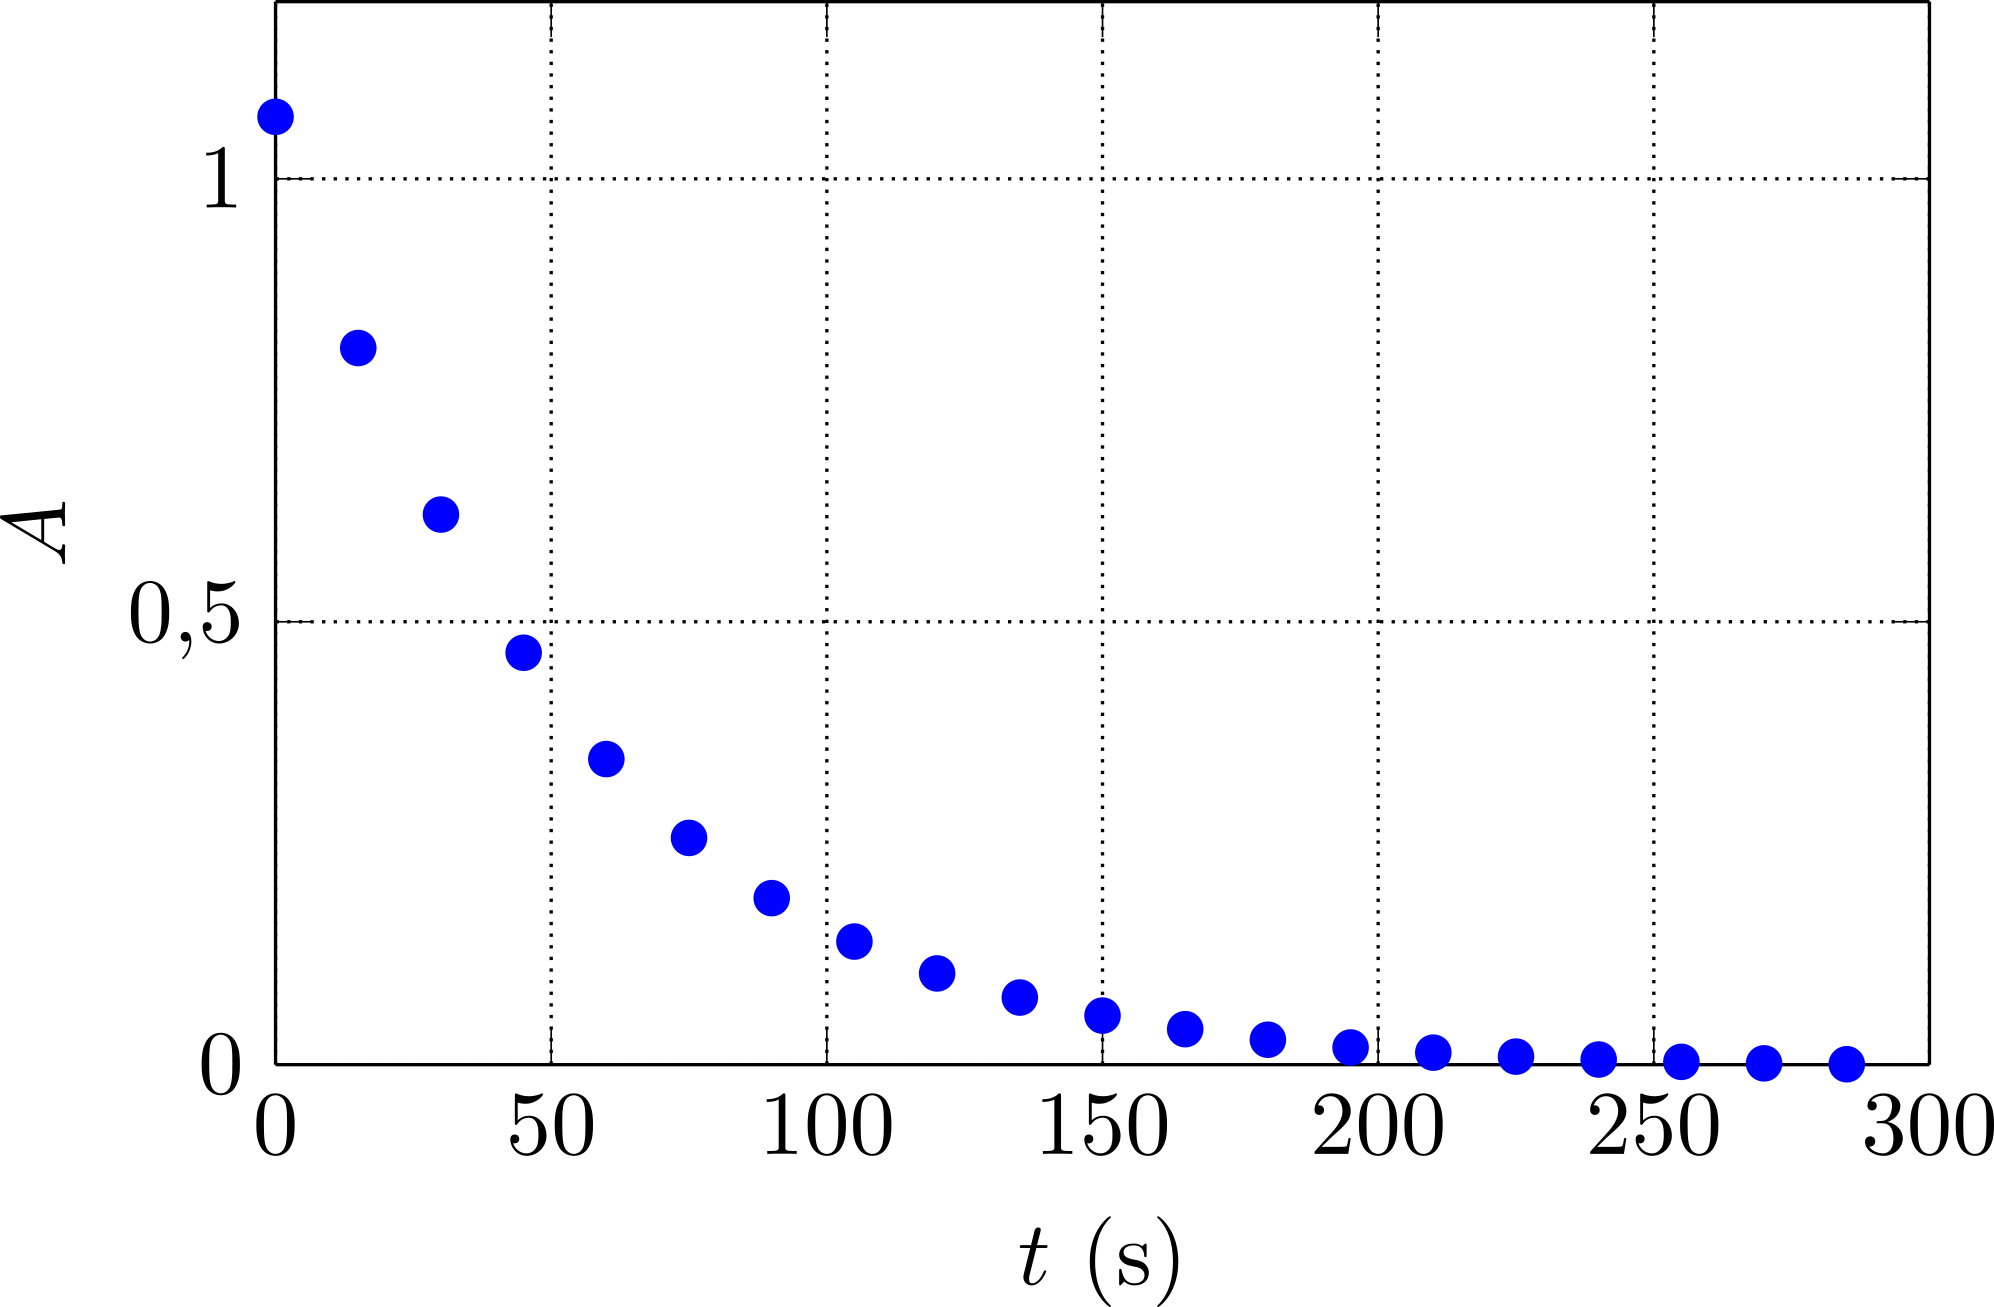
\includegraphics[width=\linewidth]{ph_evol-a}
	\end{center}
\end{minipage}
\begin{minipage}{0.49\linewidth}
	\begin{center}
		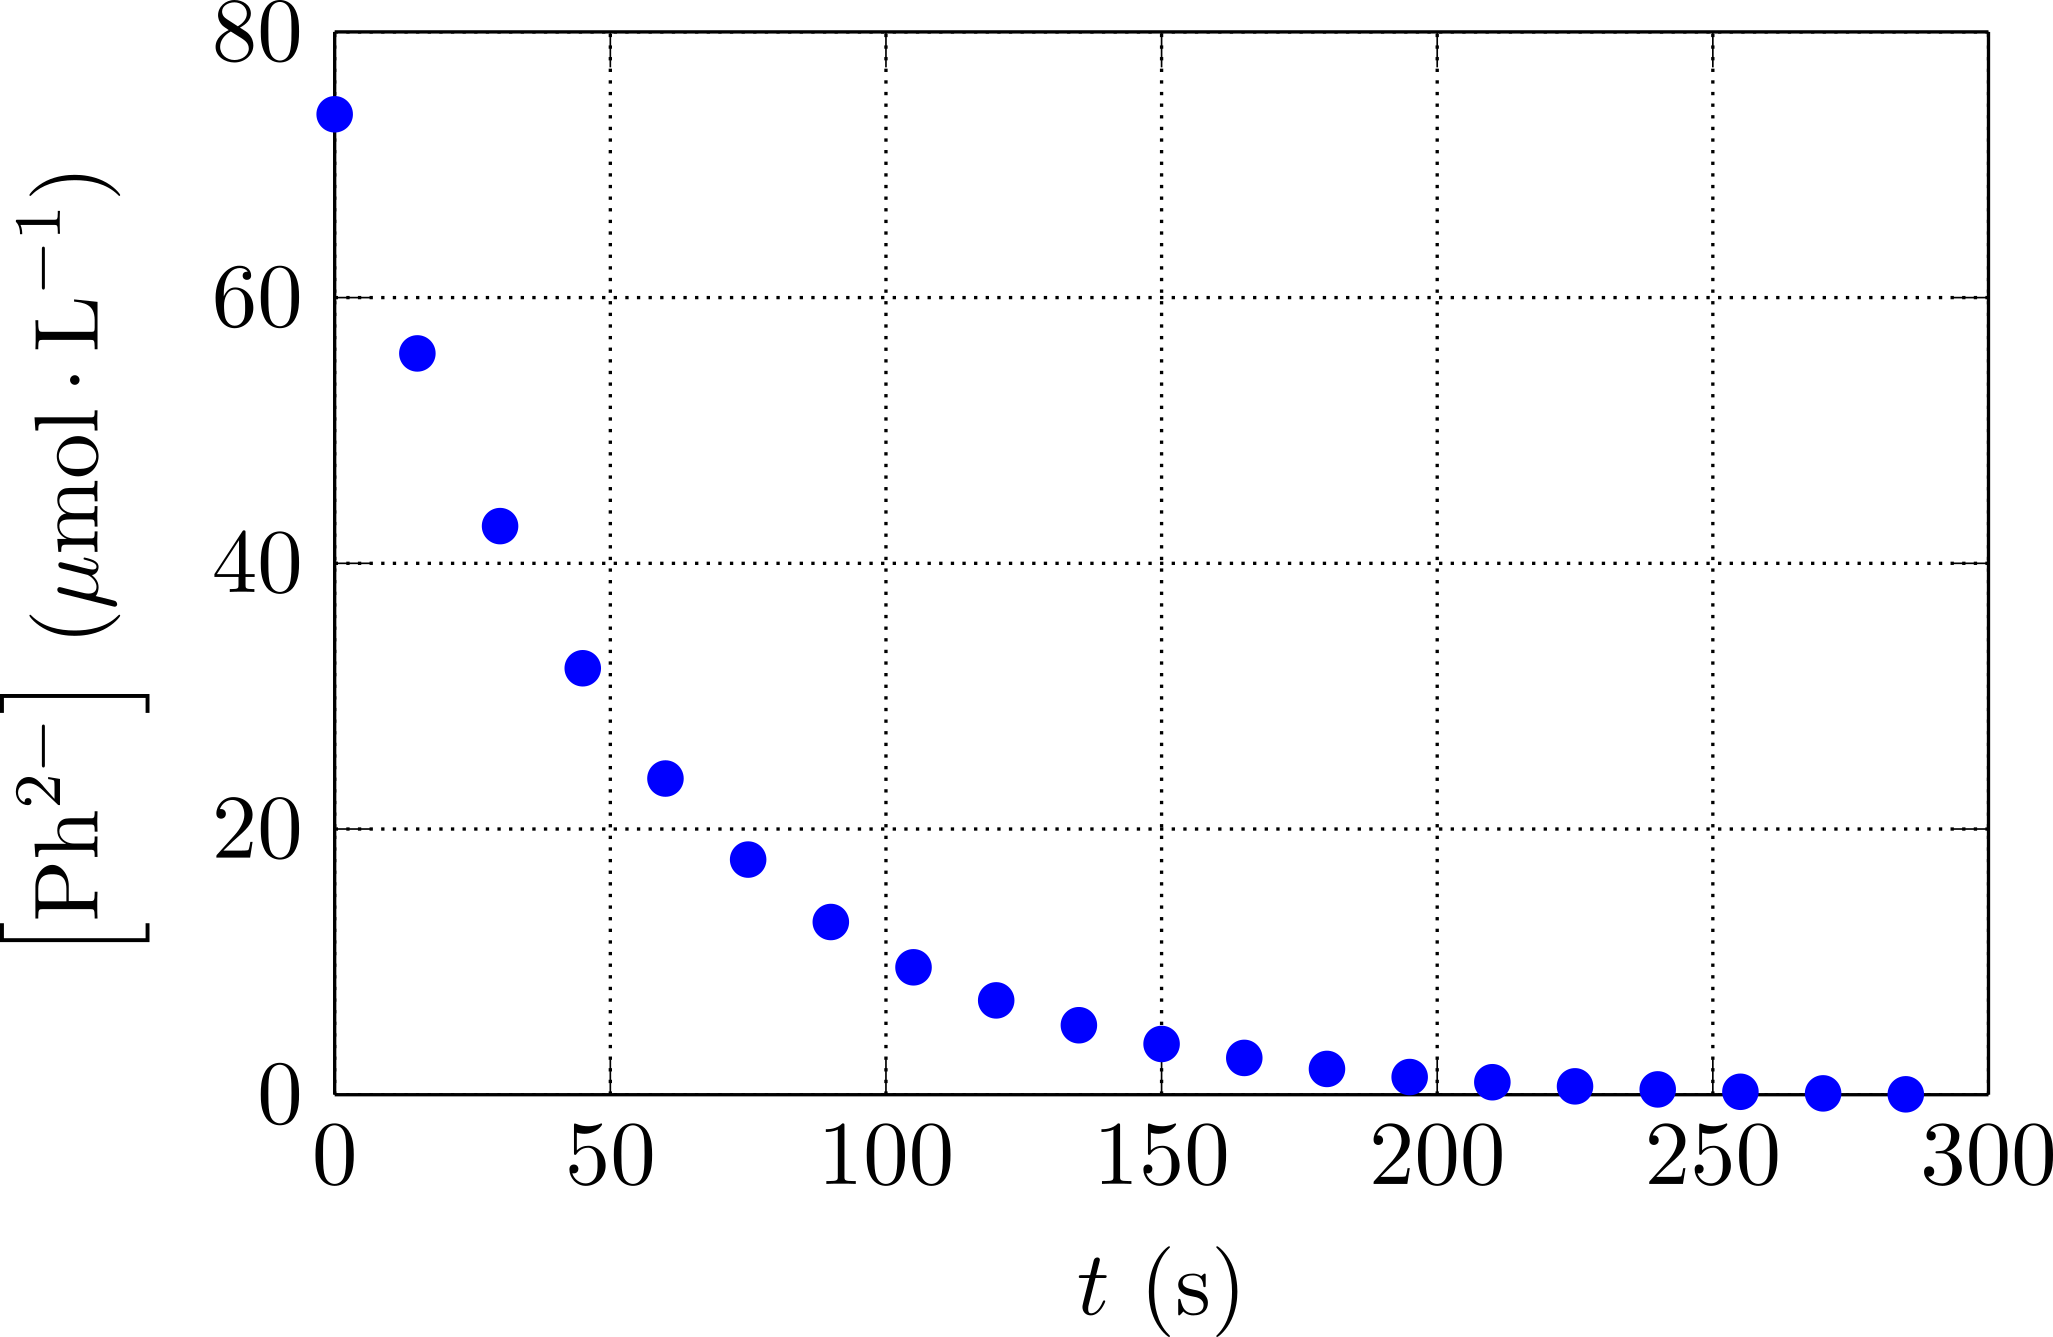
\includegraphics[width=\linewidth]{ph_evol-b}
	\end{center}
\end{minipage}

On établit le tableau d'avancement~:

\begin{center}
	\def\rhgt{0.50}
	\centering
	\begin{tabularx}{\linewidth}{|l|c||YdYdY|}
		\hline
		\multicolumn{2}{|c||}{
			$\xmathstrut{\rhgt}$
		\textbf{Équation}}           &
		$\ce{Ph^{2-}_{\aqu}}$        & $+$     &
		$\ce{HO^{-}_{\aqu}}$         & $=$     &
		$\ce{PhOH^{3-}_{\aqu}}$                  \\
		\hline
		$\xmathstrut{\rhgt}$
		Initial                      & $x = 0$ &
		\psw{$[\ce{Ph^{2-}}]_0$}     & \vline  &
		\psw{$[\ce{HO^{-}}]_0$}      & \vline  &
		$0$                                      \\
		\hline
		$\xmathstrut{\rhgt}$
		Interm.                      & $x$     &
		\psw{$[\ce{Ph^{2-}}]_0 - x$} & \vline  &
		\psw{$[\ce{HO^{-}}]_0 - x$}  & \vline  &
		\psw{$x$}                                \\
		\hline
	\end{tabularx}
\end{center}

\leftcentersright{%
D'où on tire
}{%
\psw{%
$[\ce{Ph^{2-}}] = [\ce{Ph^{2-}}]_0 - x \Lra x = [\ce{Ph^{2-}}]_0 - [\ce{Ph^{2-}}]$
}
}{%
donnant la courbe~:
}

\begin{center}
	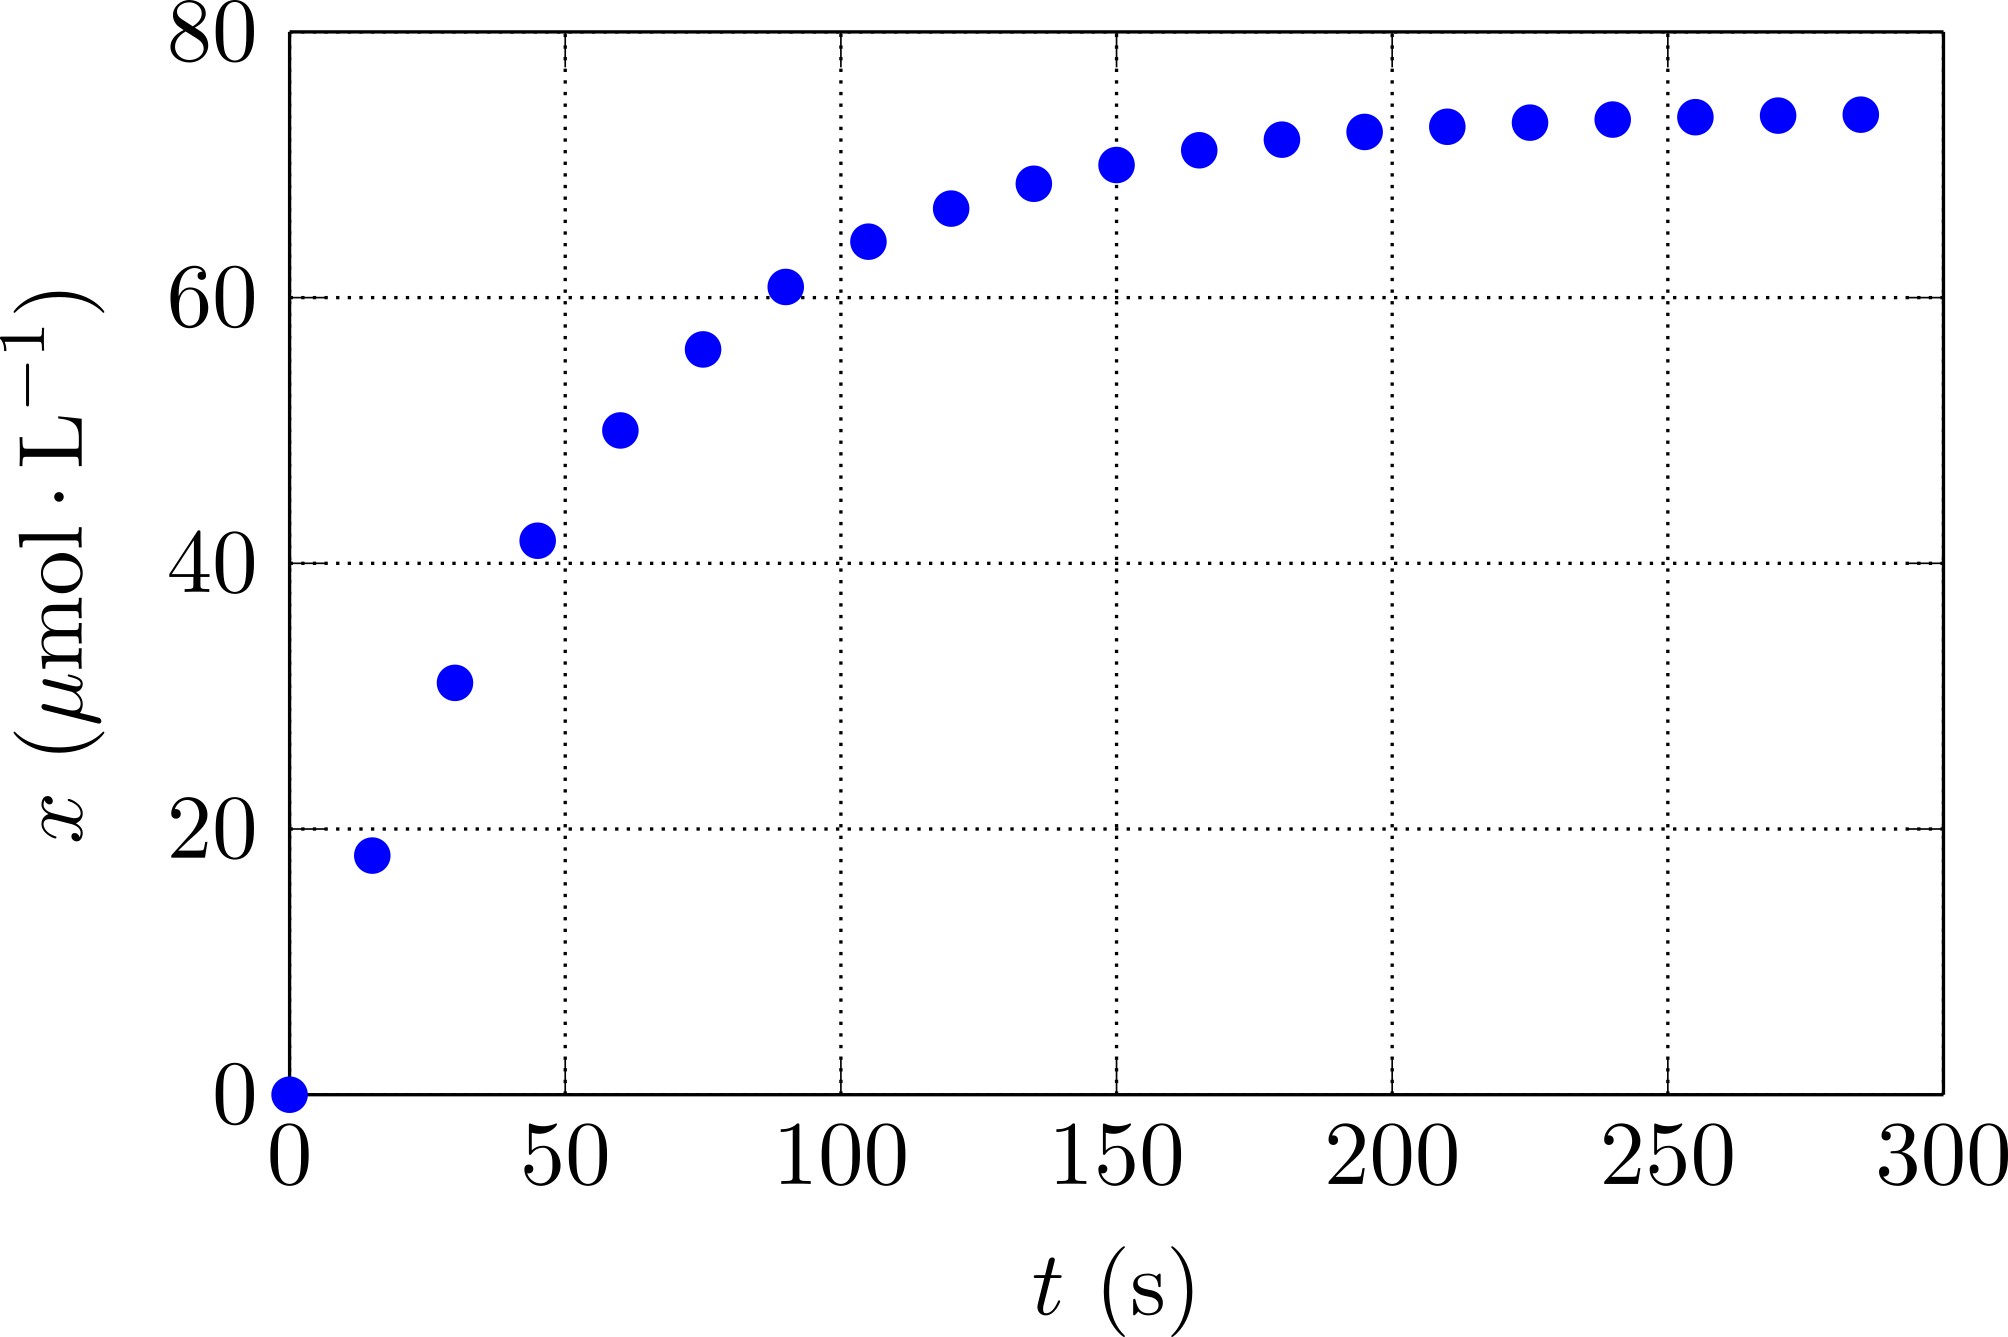
\includegraphics[width=.5\linewidth]{ph_evol-c}
\end{center}

L'avancement augmente bien avec le temps, mais on voit qu'il augmente
\textbf{plus vite au début} de la réaction qu'à la fin. En prenant la
\textbf{dérivée} de cette évolution, on trouve donc la \textbf{vitesse de
	l'avancement} $v = \dd x/\dd t$. Tracer cette grandeur en fonction du temps puis
en fonction de $[\ce{Ph^{2-}}]$ donne~:

\begin{minipage}{0.49\linewidth}
	\begin{center}
		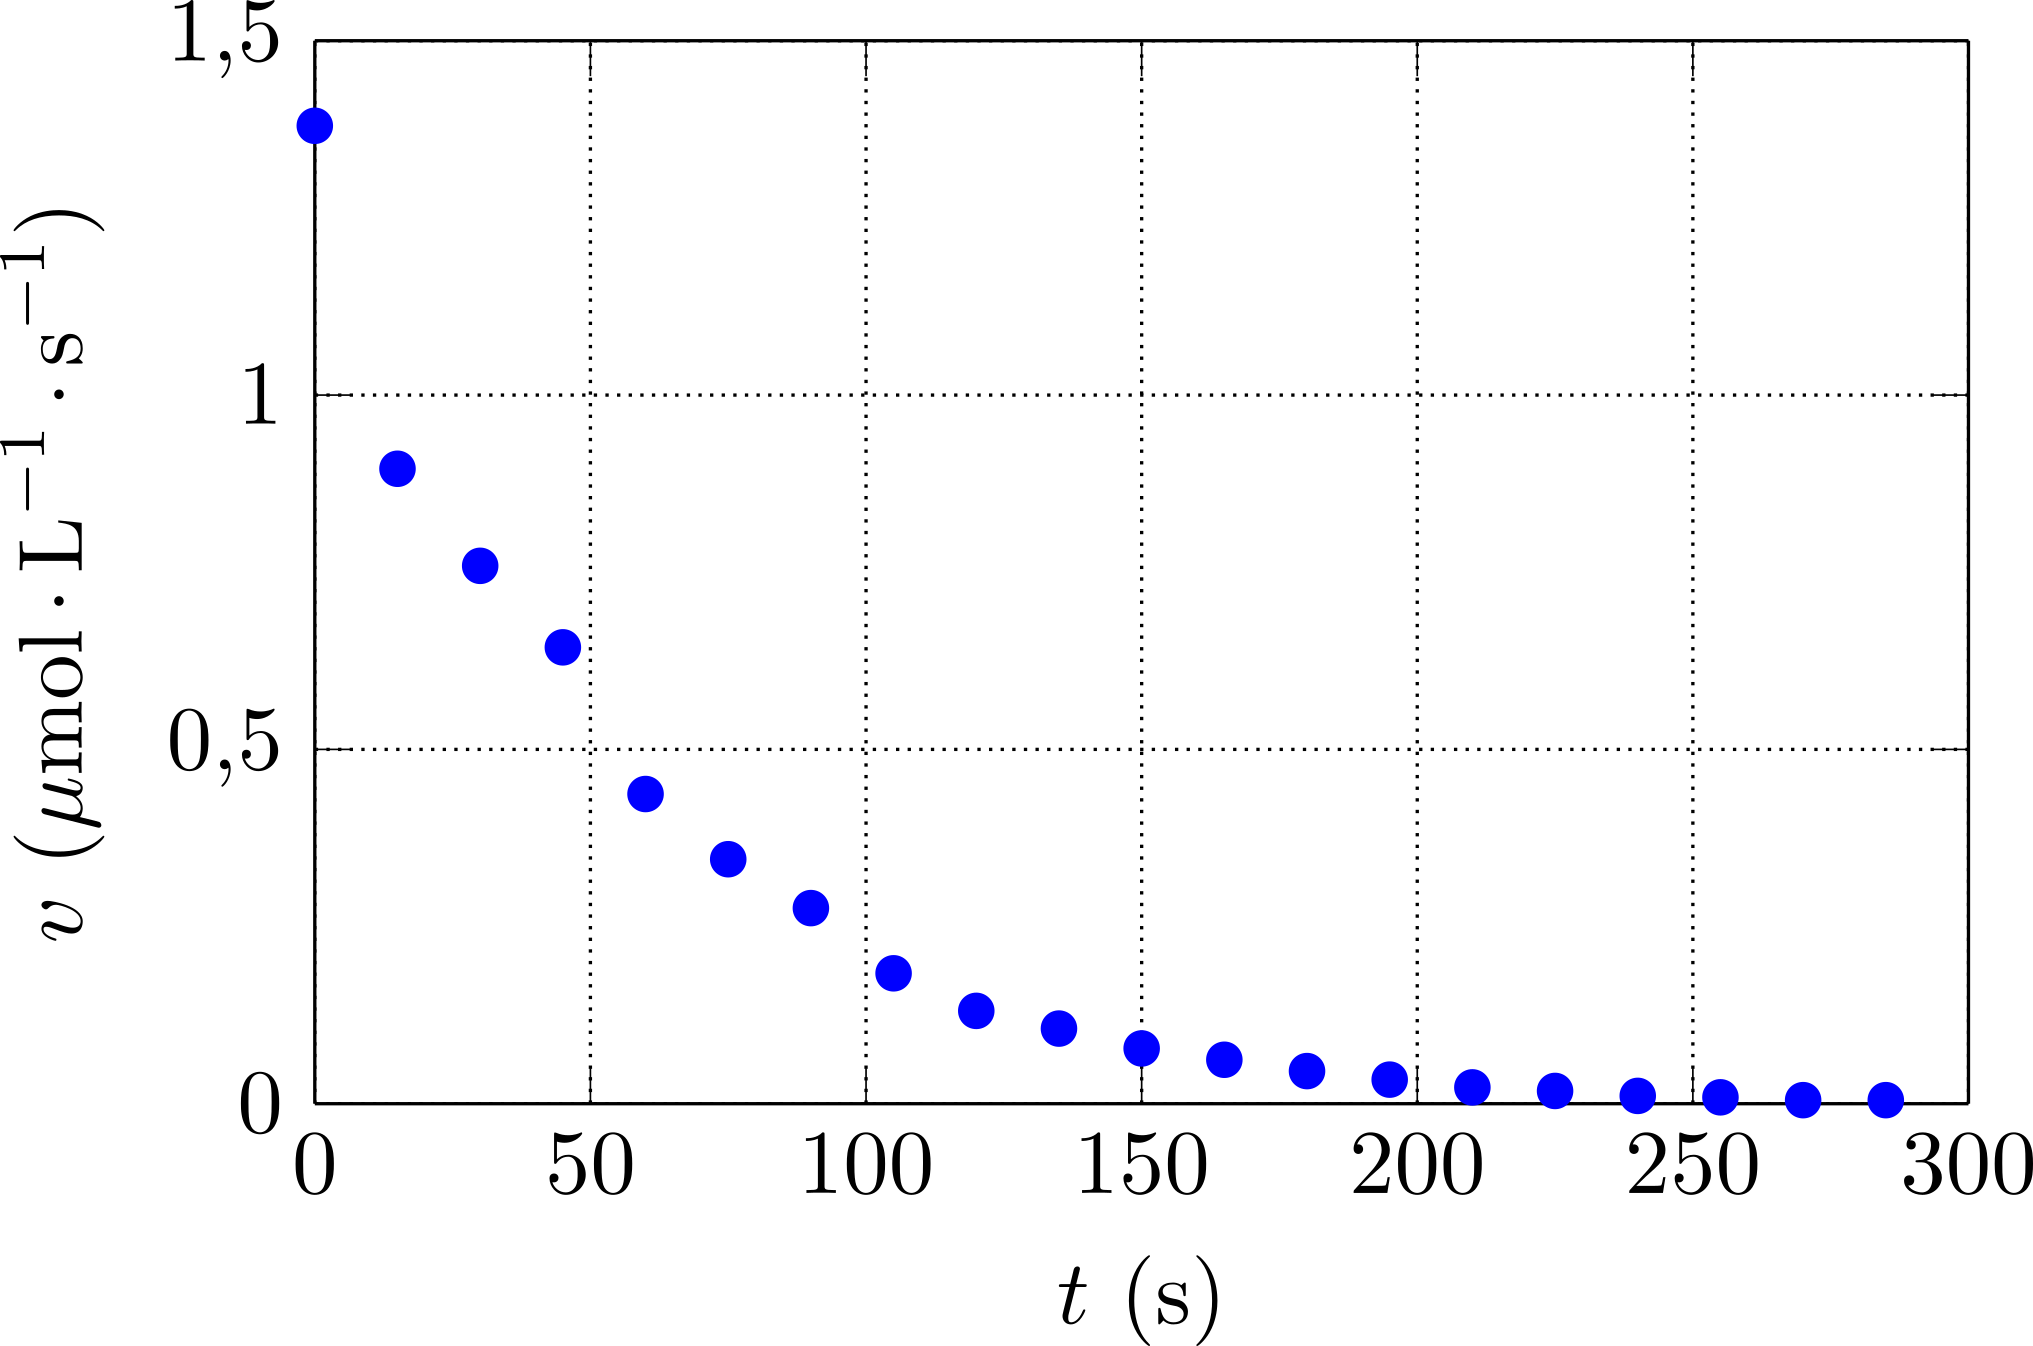
\includegraphics[width=\linewidth]{ph_evol-d}
	\end{center}
\end{minipage}
\begin{minipage}{0.49\linewidth}
	\begin{center}
		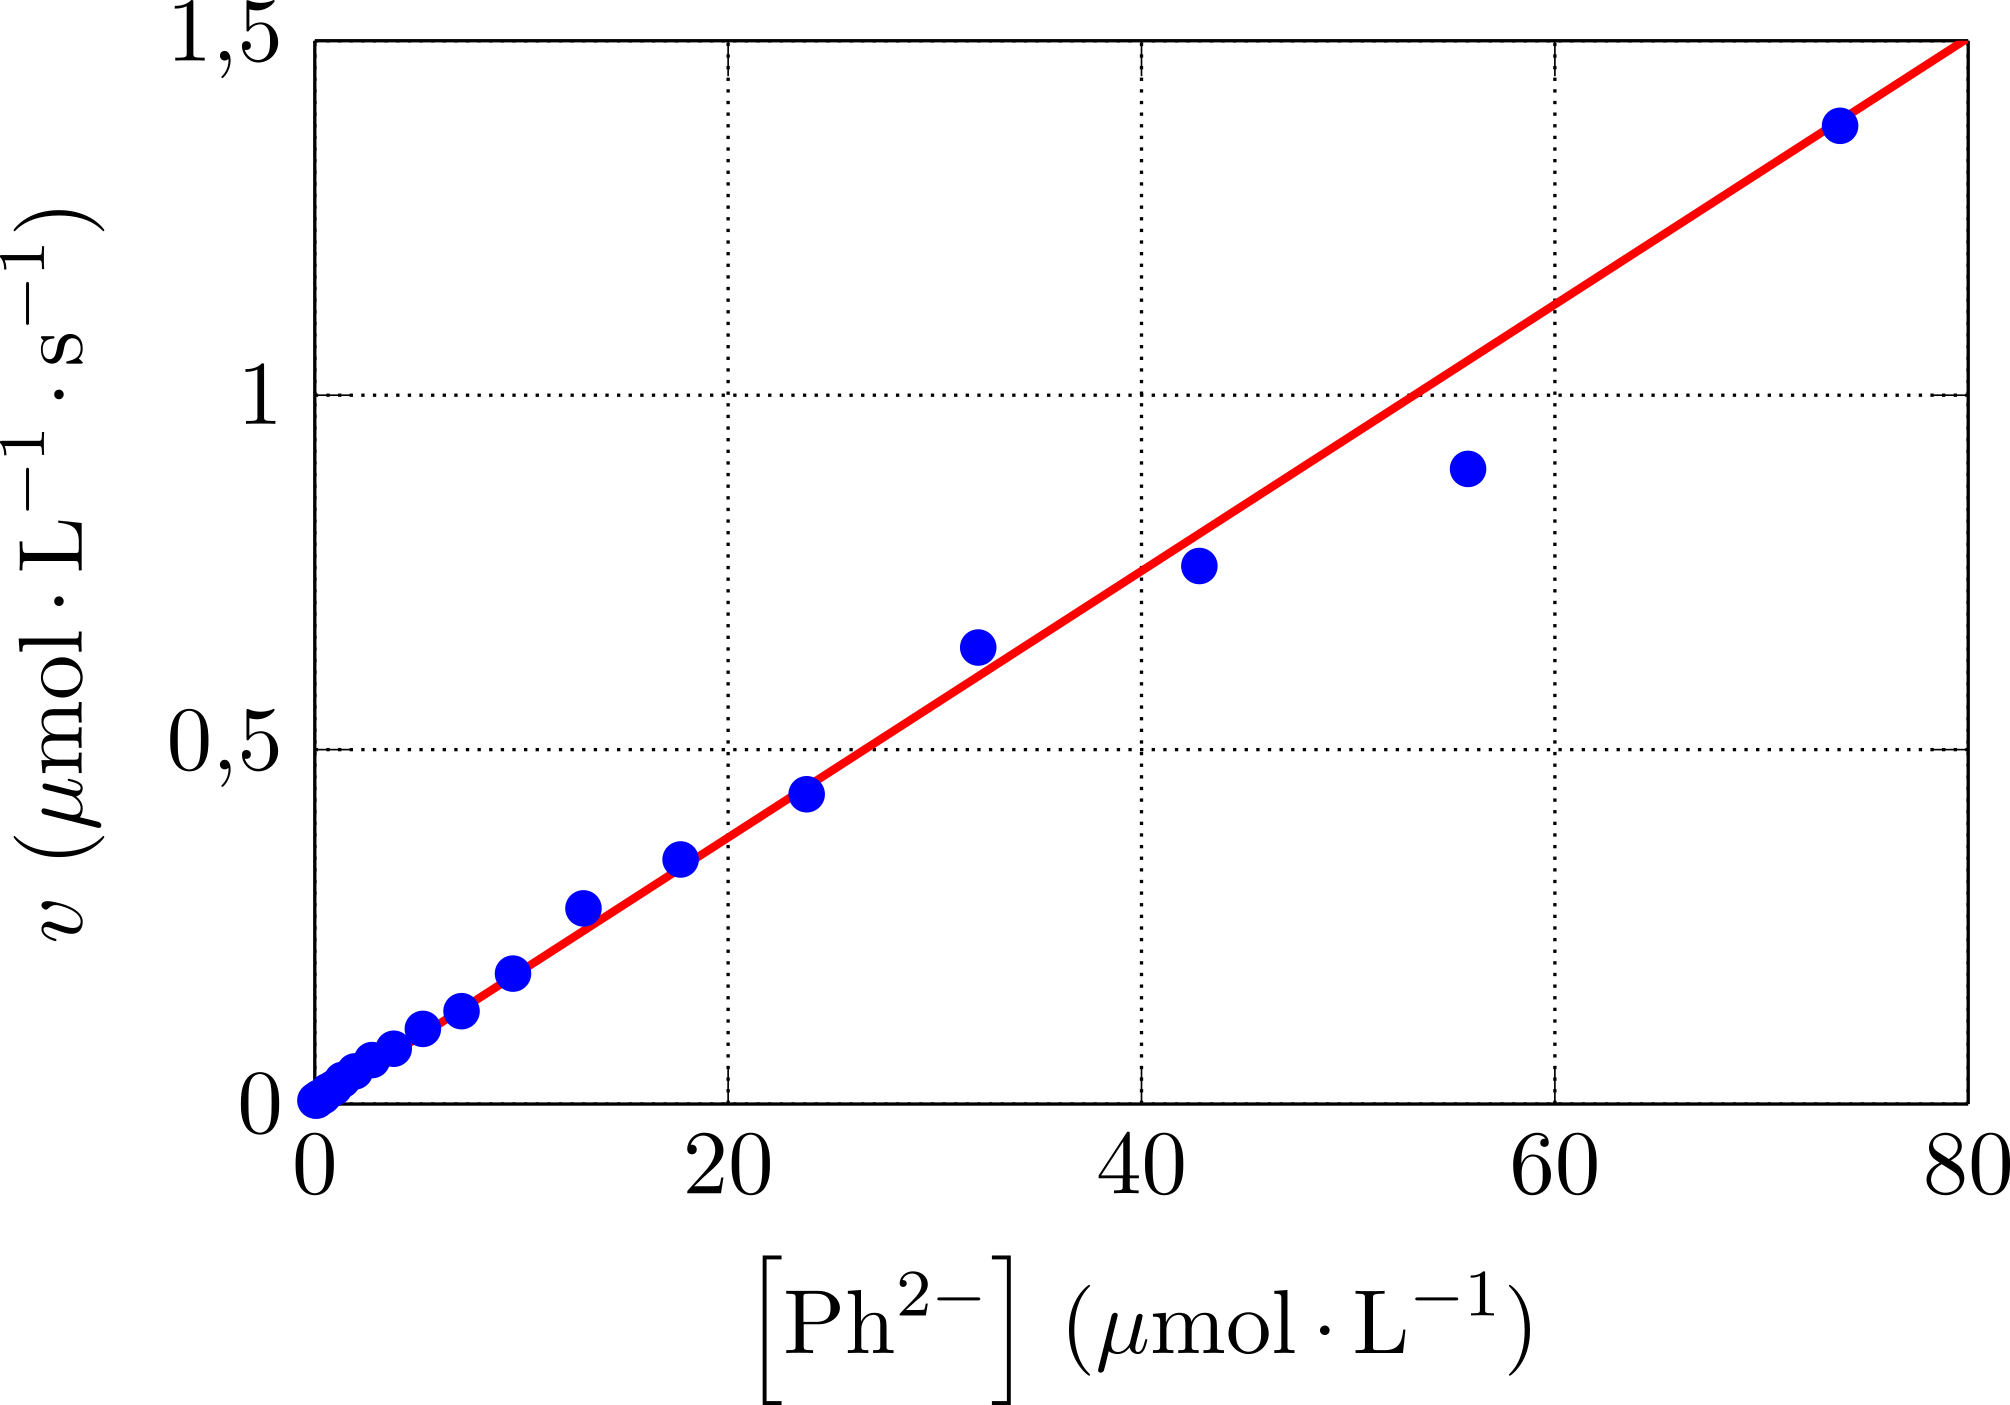
\includegraphics[width=\linewidth]{ph_evol-e}
	\end{center}
\end{minipage}

Ainsi, \textbf{dans cet exemple} de réaction et avec $[\ce{HO^{-}}]_0 =
	\SI{1}{mol.L^{-1}}$, on a $v = k[\ce{Ph^{2-}}]$ avec $k =
	\SI{1.88e-2}{s^{-1}}$. La même étude avec $[\ce{HO^{-}}]_0 =
	\SI{0.4}{mol.L^{-1}}$ donne $k = \SI{7.0e-3}{s^{-1}}$, c'est-à-dire une vitesse
plus faible que précédemment.

\section{Facteurs cinétiques}

\subsection{Présentation}

À partir de l'expérience précédente, on note qu'une \textit{augmentation de la
	concentration de soude accélère la réaction}. L'avancement a atteint la moitié
de sa valeur finale en \SI{38}{s} avec une concentration de
$\SI{1.0}{mol.L^{-1}}$, et en \SI{1}{min} \SI{30}{s} pour une concentration de
$\SI{0.4}{mol.L^{-1}}$~: c'est donc un \textbf{facteur cinétique}. On en recense
4~:

\begin{tcb*}[label=prop:factciné, breakable](prop){Facteurs cinétiques}
	Plusieurs facteurs influencent la vitesse d'une réaction donnée~:
	\begin{itemize}
		\item \psw{%
			      La concentration des réactifs~: $[\ce{R_i}] \nearrow
				      \Rightarrow v \nearrow$~;
		      }%
		\item \psw{%
			      La température~: $T \nearrow \Rightarrow v \nearrow$~;
		      }%
		\item \psw{%
			      La présence de catalyseurs, qui permettent d'accélérer une
			      réaction sans l'altérer~;
		      }%
		\item \psw{%
			      Le solvant utilisé.
		      }%
	\end{itemize}
\end{tcb*}

On peut comprendre cela avec la notion de \textbf{choc efficace}~:

\begin{tcb*}(defi){Choc efficace}
	Pour qu'une réaction ait lieu, il faut que deux molécules entrent en contact
	et ce avec suffisamment d'énergie. La vitesse de réaction dépend donc de la
	probabilité que deux molécules se choquent, et que ce choc soit efficace.
	\begin{itemize}
		\item \psw{%
			      Plus concentration $\nearrow$, plus la probabilité qu'un réactif
			      entre en contact avec un autre $\nearrow$.
		      }%
		\item \psw{%
			      Plus la température $\nearrow$, plus la vitesse des molécules
			      $\nearrow$~: la fréquence des chocs augmente et la probabilité que ces
			      chocs soient efficaces aussi.
		      }%
	\end{itemize}
\end{tcb*}

\subsection{Température et loi d'\textsc{Arrhénius}}
\subsubsection{Phénoménologie}

En effet, dans le milieu réactionnel, les molécules ont une distribution de
vitesse répartie autour d'une valeur moyenne, $v^*$, comme présenté ci-dessous à
gauche~; celles qui ont la plus grande vitesse et donc énergie cinétique ont la
capacité de passer la barrière de potentielle nécessaire à la réaction,
représentée ci-dessous à droite. Plus la \textbf{température est élevée}, plus la
proportion de \textbf{molécules pouvant passer cette barrière} est élevée.

\begin{minipage}{0.49\linewidth}
	\sswitch{
		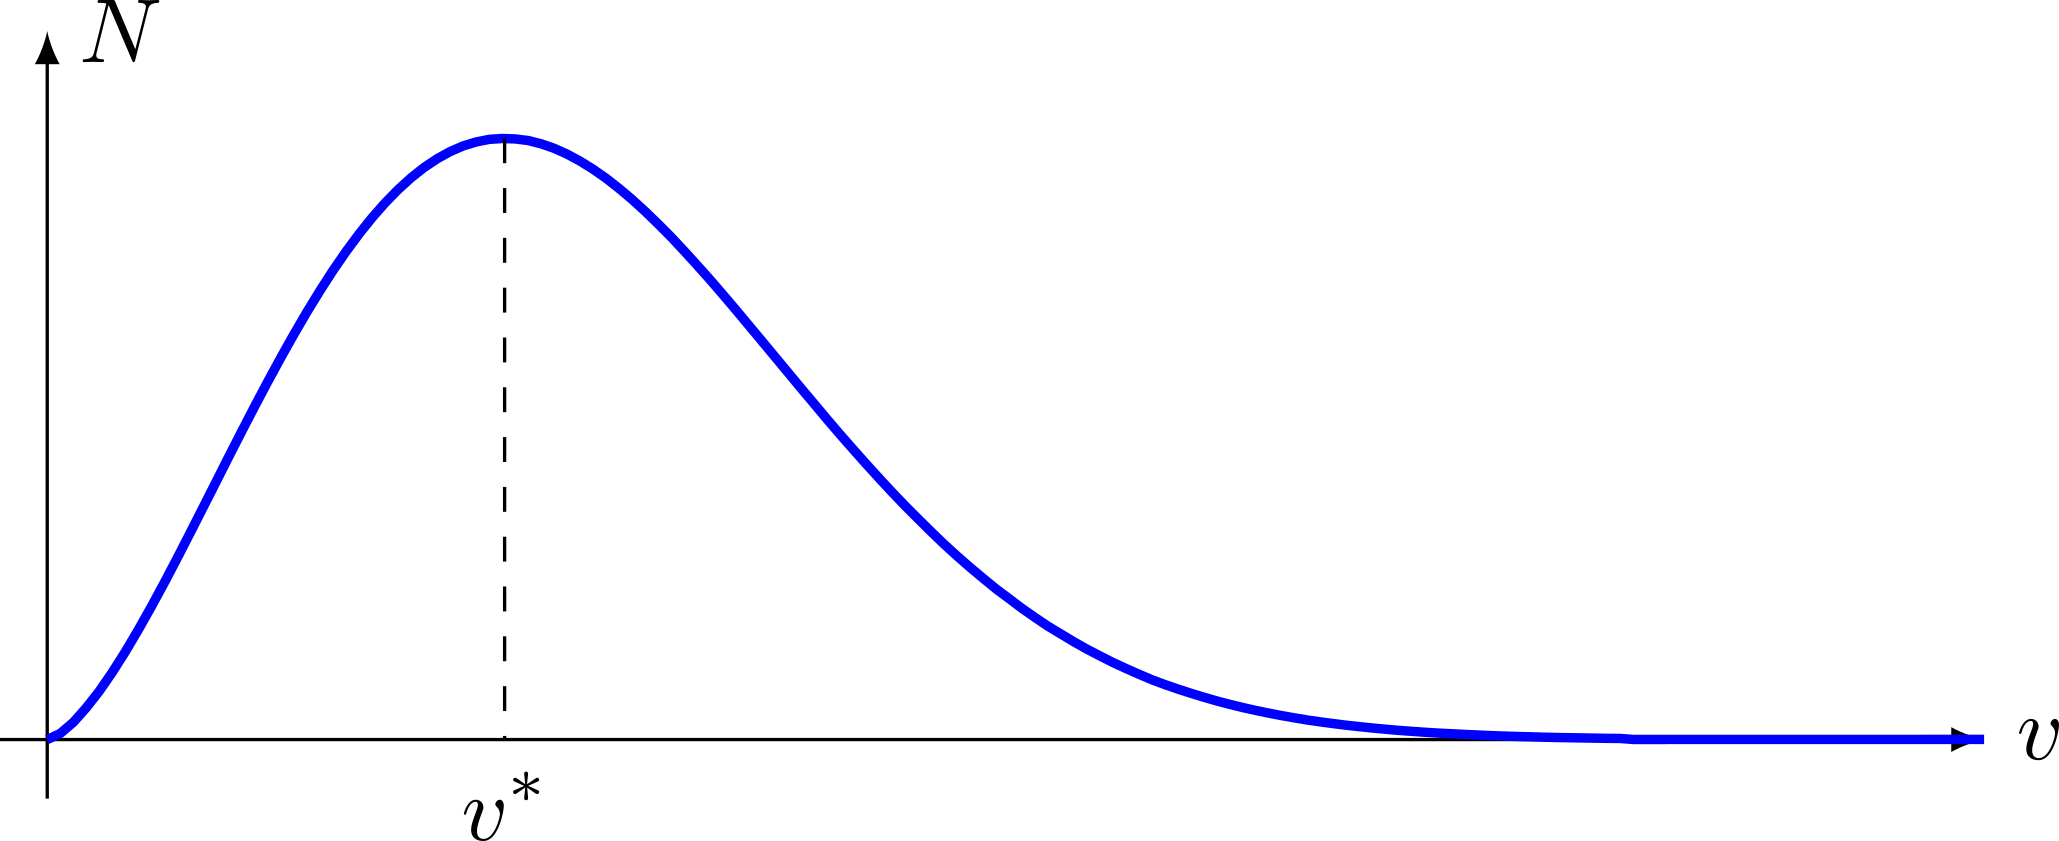
\includegraphics[height=3.5cm, draft=true]{arrh_vitesses}
	}{
		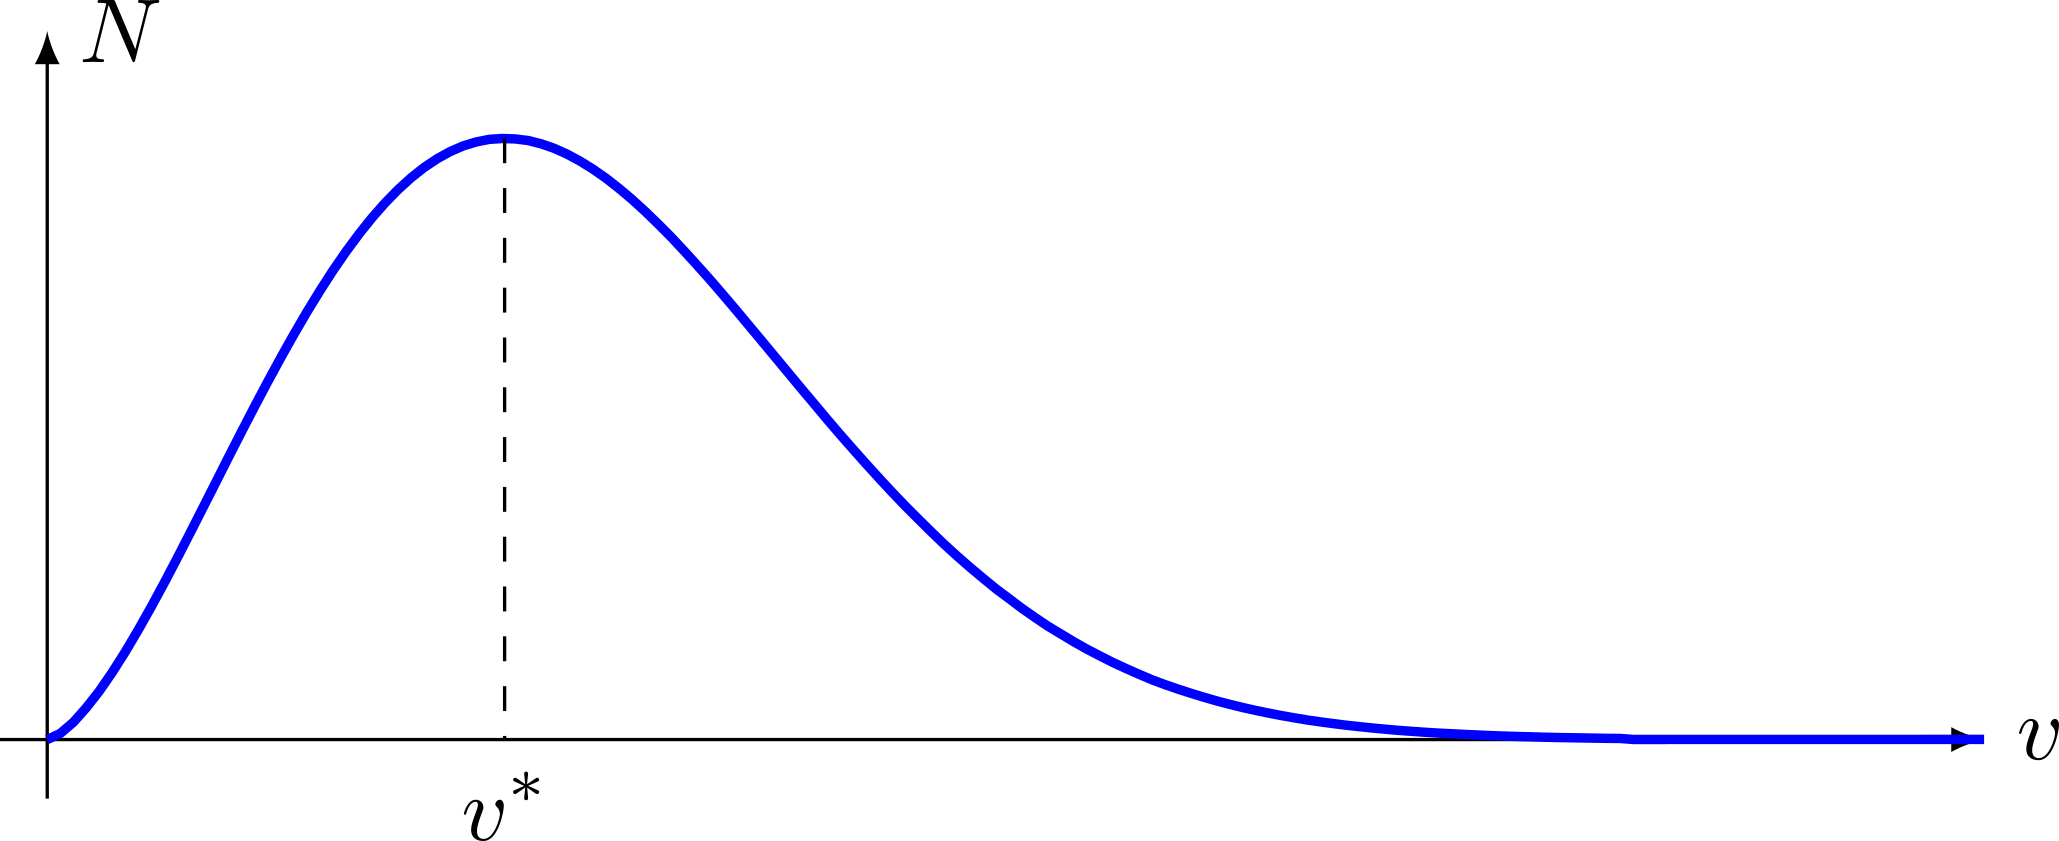
\includegraphics[height=3.5cm]{arrh_vitesses}
	}%
	\captionof{figure}{Distribution des vitesses.}
\end{minipage}
\hfill
\begin{minipage}{0.49\linewidth}
	\sswitch{
		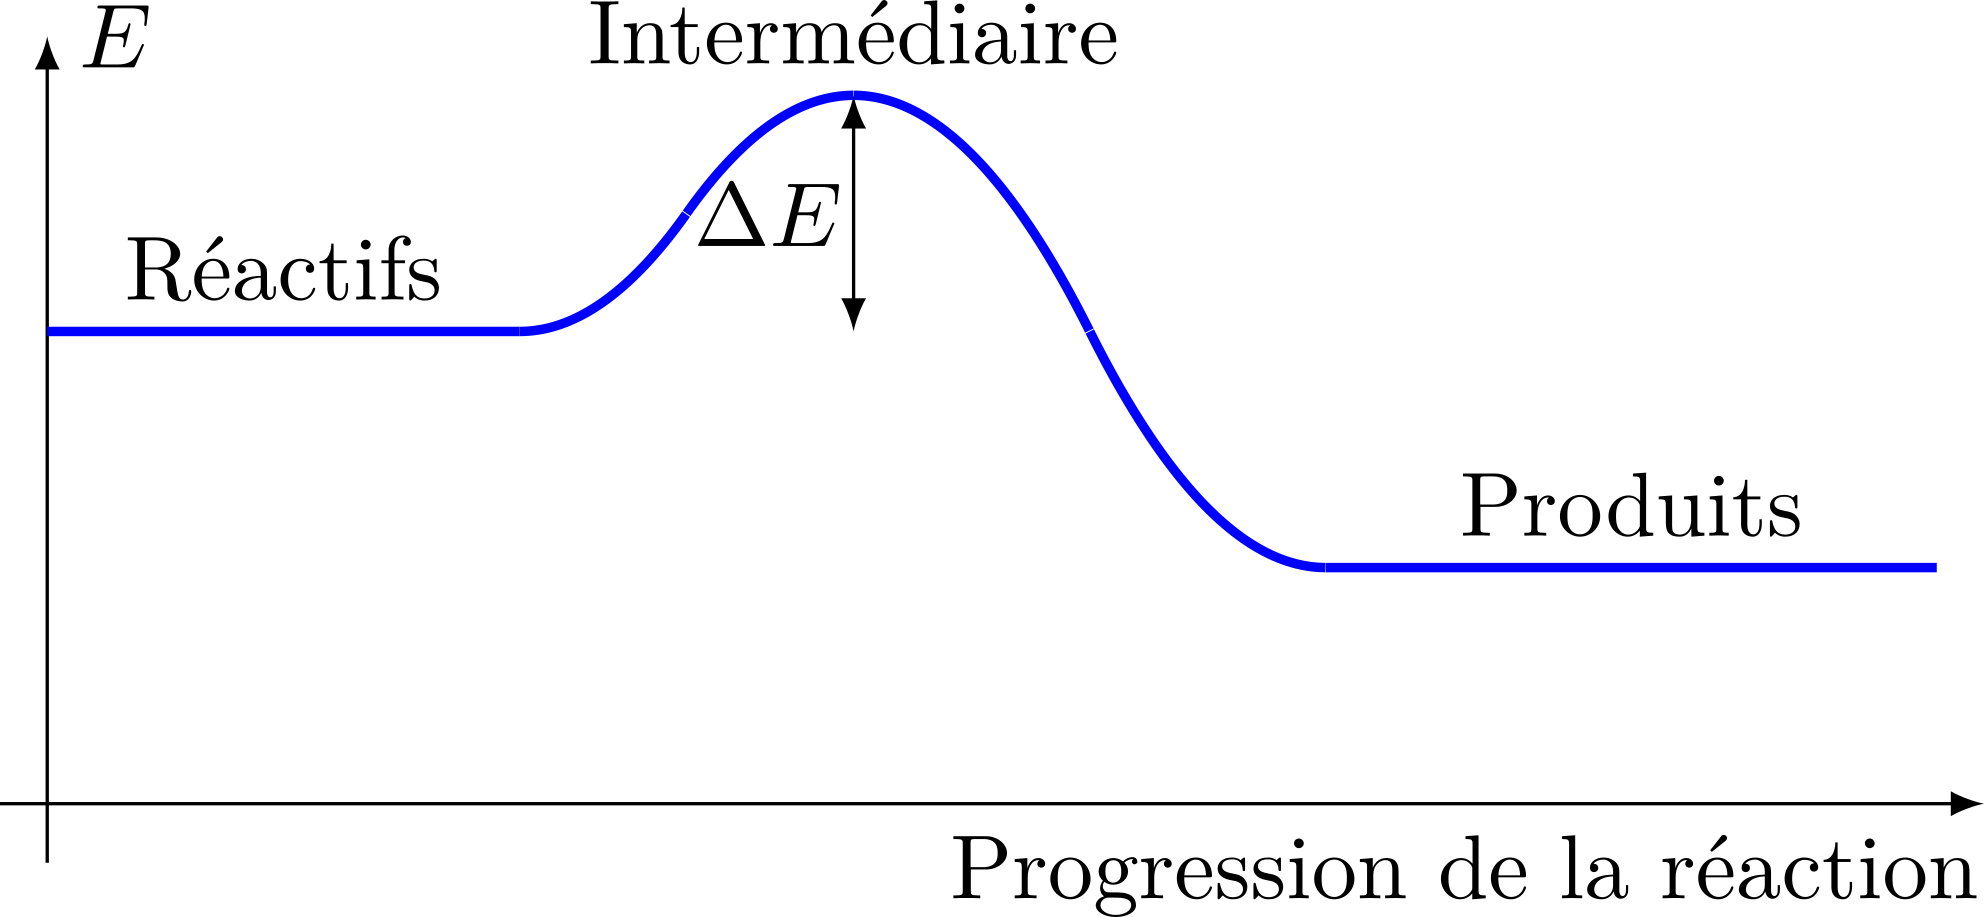
\includegraphics[height=3.5cm, draft=true]{arrh_ea}
	}{
		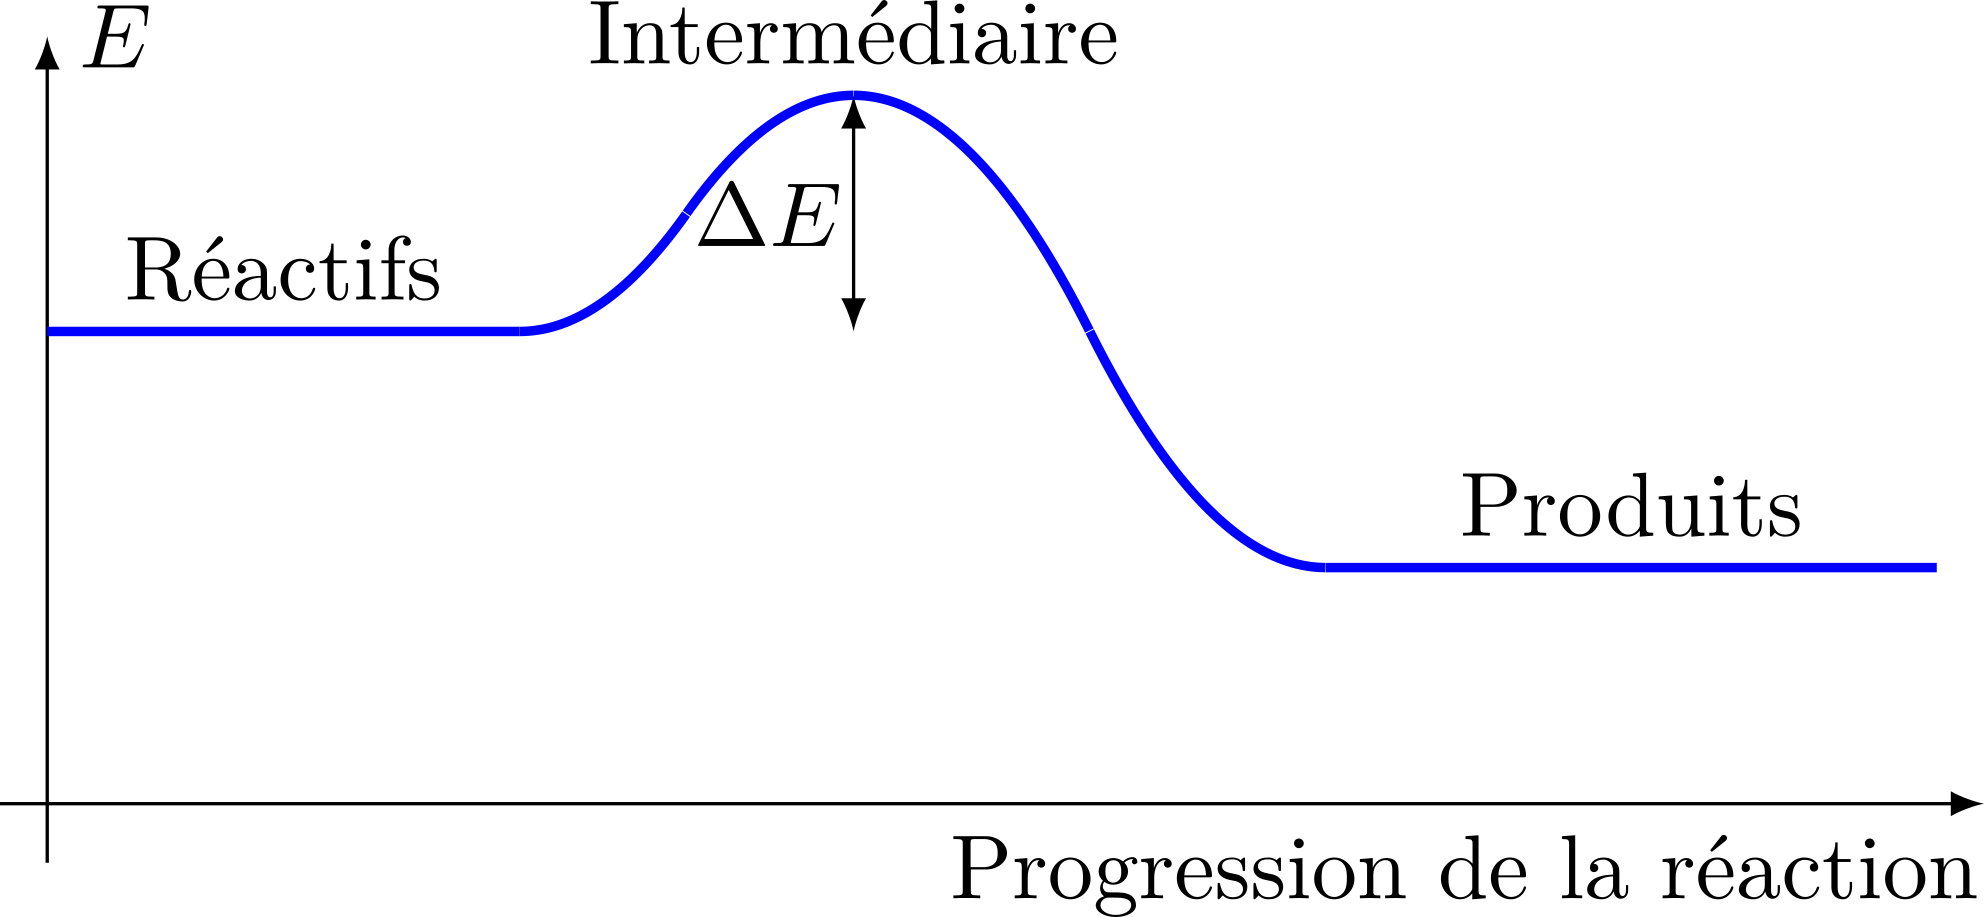
\includegraphics[height=3.5cm]{arrh_ea}
	}%
	\captionof{figure}{Barrière d'activation chimique.}
\end{minipage}

\subsubsection{Loi et utilisations}

L'évolution de la constante de vitesse suit une loi analytique en fonction de la
température, appelée \textbf{loi d'Arrhénius}~:
\begin{tcb}[label=loi:arrhenius, breakable](loi){Loi d'\textsc{Arrhénius}}
	La constante de vitesse d'une réaction chimique vérifie la loi empirique
	d'\textsc{Arrhénius}~:
	\psw{%
		\[\boxed{k(T) = A\exp \left( - \frac{\Ec_a}{RT} \right)}\]
	}%
	\vspace{-15pt}
	\begin{itemize}
		\item \psw{%
			      $A$ est le facteur pré-exponentiel, de même unité que $k$~;
		      }%
		\item \psw{%
			      $\Ec_a$ est une grandeur positive appelée \textbf{énergie d'activation},
			      en $\si{J.mol^{-1}}$~;
		      }%
		\item \psw{%
			      $R$ est la constante des gaz parfaits, et $T$ la température en Kelvins.
		      }%
	\end{itemize}
\end{tcb}

\begin{tcb*}[breakable](tool){Utilisations de la loi d'\textsc{Arrhénius}}
	On peut utiliser cette loi pour \textbf{trouver l'énergie d'activation} d'une réaction,
	ou à l'inverse \textbf{déterminer la constante de vitesse} d'une réaction.
	\begin{itemize}
		\item[b]{Avec deux températures}:
		      Supposons qu'on a effectué le suivi cinétique d'une
		      même réaction à deux températures, $T_1$ et $T_2$, et déterminé $k(T_1)$ et
		      $k(T_2)$. D'après la loi d'\textsc{Arrhénius}, on a donc
		      \psw{%
			      \begin{gather*}
				      \frac{k(T_1)}{k(T_2)}
				      = \frac{A \exp \left( - \dfrac{\Ec_a}{RT_1} \right)}{A
					      \exp \left( - \dfrac{\Ec_a}{RT_2} \right)}
				      = \exp \left( \frac{\Ec_a}{R} \left(
					      \frac{1}{T_2} - \frac{1}{T_1} \right) \right)
				      \\\Lra
				      \boxed{\Ec_a = R \frac{T_1T_2}{T_1-T_2}\ln \left( \frac{k(T_1)}{k(T_2)} \right)}
			      \end{gather*}
		      }%
		\item[b]{Succession de températures}:
		      Avec une succession de températures, on peut tracer la régression linéaire~:
		      \psw{%
			      \[
				      y\tikzmark{yn} = a\tikzmark{an}x\tikzmark{xn} + b\tikzmark{bn}
			      \]
			      \tikz[remember picture, overlay]
			      \draw[-stealth, transform canvas={xshift=-6pt, yshift=-6pt}]
			      (pic cs:yn) --++ (-10pt,-10pt)
			      node[anchor=north east] {$\ln (k(T))$}
			      ;
			      \tikz[remember picture, overlay]
			      \draw[-stealth, transform canvas={xshift=-5pt, yshift=-6pt}]
			      (pic cs:an) --++(-5pt,-10pt)
			      node[anchor=north] {$-\frac{\Ec_a}{R}$}
			      ;
			      \tikz[remember picture, overlay]
			      \draw[-stealth, transform canvas={xshift=0pt, yshift=-6pt}]
			      (pic cs:xn) --++(5pt,-10pt)
			      node[anchor=north] {$\frac{1}{T}$}
			      ;
			      \tikz[remember picture, overlay]
			      \draw[-stealth, transform canvas={xshift=3pt, yshift=-6pt}]
			      (pic cs:bn) --++(10pt,-10pt)
			      node[anchor=north west] {$\ln (A)$}
			      ;
		      }
		      \vspace{15pt}
	\end{itemize}
\end{tcb*}

\section{Vitesse(s) de réaction}
\subsection{Hypothèses de travail}
Pour la définition formelle de l'étude de la cinétique, on pose le cadre
d'étude. Les systèmes physico-chimiques considérés seront tous~:
\begin{tcb}(defi){Cadre de travail}
	\begin{itemize}
		\item \psw{%
			      \textbf{fermés} (pas d'échange de matière)~;
		      }%
		\item \psw{%
			      \textbf{isothermes} (température constante)~;
		      }%
		\item \psw{%
			      \textbf{isobares} (pression constante)~;
		      }%
		\item \psw{%
			      \textbf{homogènes} (avec une unique phase).
		      }%
		\item \psw{%
			      et surtout \textbf{à volume constant}.
		      }%
	\end{itemize}
\end{tcb}

\subsection{Vitesse de réaction}

Pour définir la vitesse d'une réaction de manière satisfaisante, elle doit être
\textbf{indépendante de l'espèce chimique suivie}~: pour caractériser la
réaction on utilisera donc l'\textbf{avancement} de la réaction. Il aussi
souhaitable que la vitesse soit intensive, donc ne dépende pas de la taille du
système~: on s'intéresse donc à l'avancement \textbf{volumique} $x = \xi/V$.
Ainsi,
\begin{tcb*}[label=def:vreac, sidebyside, righthand ratio=.3](defi)
	{Vitesse de réaction}
	On définit la vitesse d'une réaction par
	\psw{%
		\[\boxed{
				v = \dv{x}{t}} \qavec \boxed{x = \frac{\xi}{V}}\]
	}%
	\vspace{-15pt}
	\tcblower
	\tcbsubtitle{\fatbox{Unité}}
	\psw{%
	\[
		[v] = \si{mol.L^{-1}.s^{-1}}
	\]
	}%
	\vspace{-15pt}
\end{tcb*}

On trouve aussi parfois la notation $r$ pour la vitesse, pour la
différencier de la vitesse en mécanique et ne pas confondre $x$ avec
la position d'un corps massique.

\subsection{Vitesses de formation/disparition}

En plus de la vitesse de réaction, on peut en effet définir la vitesse de
formation d'un produit, ou de disparition d'une espèce.
\begin{tcb*}[label=def:vfordisp](defi){Vitesses formation, disparition}
	\leftcenters{%
		Pour une réaction
	}{%
		$
			\ce{\alpha_1R_1 + \alpha_2R_2} +…
			=
			\ce{\beta_1P_1 +\beta_2P_2}+…
		$
	}%
	\begin{isd}
		La vitesse de formation d'un produit est
		\psw{%
			\[\boxed{v_{f,\ce{P}} = \dv{[\ce{P}]}{t}}\]
		}%
		\tcblower
		La vitesse de disparition d'un réactif est
		\psw{%
			\[\boxed{v_{d,\ce{R}} = -\dv{[\ce{R}]}{t}}\]
		}%
		\textbf{Attention au signe «~$-$~»~}: le réactif disparaît, mais la
		\textbf{vitesse} doit être \textbf{positive}.
	\end{isd}
	\vspace{-15pt}
\end{tcb*}

\begin{tcb*}[label=prop:vreacfordisp](prop){Lien entre les vitesses}
	\leftcentersright{%
		Pour une réaction
	}{%
		$\DS 0 = \sum_{i} \nu_i {\ce{X}}_i$
	}{%
		on a
	}%
	% \qavec \xi = \frac{n_i - n_{i,0}}{\nu_i}\]
	\psw{%
		\[
			\boxed{v = \frac{1}{\nu_{\ce{X_i}}} \dv{[{\ce{X}}_i]}{t}}
			\Lra
			\boxed{%
				v_{d,\ce{R}} = -\nu_{\ce{R_i}} v = \abs{\nu_{\ce{R_i}}} v
			}%
			\qet
			\boxed{%
				v_{f,\ce{P}} = \nu_{\ce{P_i}} v
			}
		\]
	}%
\end{tcb*}

\begin{tcb}[breakable](demo){Lien entre les vitesses}
	% On part de l'évolution de la quantité de matière d'un constituant en fonction
	% de $\xi$~:
	\psw{%
		\begin{DispWithArrows*}[]
			n_{\ce{X_i}}(t) &= n_{\ce{X_i},0} + \nu_{\ce{X_i}}\xi(t)
			\Arrow{On isole}
			\\\Lra
			\xi(t) &= \frac{n_{\ce{X_i}}(t) - n_{\ce{X_i},0}}{\nu_{\ce{X_i}}}
			\Arrow{$\mdiv V$}
			\\\Lra
			x(t) &= \frac{1}{\nu_{\ce{X_i}}} \frac{n_{\ce{X_i}}(t) - n_{\ce{X_i},0}}{V}
			\Arrow{$\DS\dv{\cdot}{t}$ et $\frac{n_{\ce{X_i}}(t)}{V} = [\ce{X_i}](t)$}
			\\\Lra
			\Aboxed{\dv{x}{t} &= \frac{1}{\nu_{\ce{X_i}}} \dv{[\ce{X_i}]}{t}}
		\end{DispWithArrows*}
	}%
	\begin{isd}[interior hidden]
		\vspace{-15pt}
		\tcbsubtitle{\fatbox{\textbf{Formation}}}
		\psw{%
			\begin{DispWithArrows*}[fleqn, mathindent=5pt]
				v_{f,\ce{P}} &= \dv{[P]}{t}
				\Arrow{$[\ce{P}](t) = [\ce{P}]_0 + \nu_{\ce{P_i}}x(t)$}
				\\\Lra
				\Aboxed{v_{f,\ce{P}} &= \nu_{\ce{P_i}} v}
			\end{DispWithArrows*}
		}%
		\tcblower
		\vspace{-15pt}
		\tcbsubtitle{\fatbox{\textbf{Disparition}}}
		\psw{%
			\begin{DispWithArrows*}[fleqn, mathindent=5pt]
				v_{d,\ce{R}} &= - \dv{[R]}{t}
				\Arrow{$[\ce{R}](t) = [\ce{R}]_0 + \nu_{\ce{R_i}}x(t)$}
				\\\Lra
				\Aboxed{v_{d,\ce{R}} &= -\nu_{\ce{R_i}} v}
			\end{DispWithArrows*}
		}%
	\end{isd}
\end{tcb}

\begin{tcb}(exem)<lftt>{Vitesses formation, disparition}
	En reprenant l'exemple précédent, on a bien
	\begin{gather*}
		v_{d,\ce{HO^{-}}}     =
		\psw{%
			- \dv{[\ce{HO^{-}}]}{t} =
			- \dv{([\ce{HO^{-}}]_0 - x)}{t} =
			v
		}
		\qqet
		v_{f,\ce{PhOH^{3-}}}  =
		\psw{%
			\dv{[\ce{PhOH^{3-}}]}{t} =
			\dv{x}{t} =
			v
		}
	\end{gather*}
\end{tcb}

% En effet, avec un tableau d'avancement général on aurait
% \begin{center}
% 	\def\rhgt{0.35}
% 	\centering
% 	\begin{tabularx}{\linewidth}{|l|c||YdYdYdY|}
% 		\hline
% 		\multicolumn{2}{|c||}{
% 			$\xmathstrut{\rhgt}$
% 		\textbf{Équation}}        &
% 		$a\ce{A}$                 & $+$     &
% 		$b\ce{B}$                 & $\ra$   &
% 		$c\ce{C}$                 & $+$     &
% 		$d\ce{D}$                             \\
% 		\hline
% 		$\xmathstrut{\rhgt}$
% 		Initial                   & $x = 0$ &
% 		$c_{\ce{A},0}$            & \vline  &
% 		$c_{\ce{B},0}$            & \vline  &
% 		$c_{\ce{C},0}$            & \vline  &
% 		$c_{\ce{D},0}$                        \\
% 		\hline
% 		$\xmathstrut{\rhgt}$
% 		Interm.                   & $x$     &
% 		\psw{$c_{\ce{A},0} - ax$} & \vline  &
% 		\psw{$c_{\ce{B},0} - bx$} & \vline  &
% 		\psw{$c_{\ce{C},0} + cx$} & \vline  &
% 		\psw{$c_{\ce{D},0} + dx$}             \\
% 		\hline
% 	\end{tabularx}
% \end{center}
% \begin{flalign*}
% 	\Ra
% 	v_{d, \ce{A}} & =
% 	\psw{%
% 		- \dv{[\ce{A}]}{t} = - \dv{(c_{\ce{A}} - ax)}{t} = av
% 	}             &
% 	\\
% 	\qet
% 	v_{f, \ce{C}} & =
% 	\psw{%
% 		\dv{[\ce{C}]}{t} = \dv{(c_{\ce{C}} + cx)}{t} = cv
% 	}             &
% 	\vspace{-15pt}
% \end{flalign*}

\begin{tcb}[breakable](appl)<lftt>{Vitesses d'une réaction}
	Écrire $v$ en fonction des concentrations pour la réaction
	\[
		\ce{6H^{+}_{\aqu} + 5Br^{-}_{\aqu} + BrO3^{-}_{\aqu}
			=
			3Br2_{\aqu} + 3H2O_{\liq}}
	\]
	\tcblower
	\psw{%
		D'après la propriété précédente, on a
		\[
			v = - \frac{1}{6} \dv{[\ce{H+}]}{t}
			= - \frac{1}{5} \dv{[\ce{Br-}]}{t}
			= - \dv{[\ce{BrO3-}]}{t}
			= \frac{1}{3} \dv{[\ce{Br2}]}{t}
		\]
	}%
	\vspace{-15pt}
\end{tcb}

\section{Concentration et ordre de réaction}
\subsection{Ordre d'une réaction}
\textit{A priori}, il n'y a \textit{pas de relation simple} permettant de
déterminer la vitesse d'une réaction en fonction des paramètres
physico-chimiques du systèmes. Cependant, il y a certaines réactions qui ont une
expression simple, comme on l'a vu en introduction. Prenons une réaction de la
forme
\[
	\psw{%
		a\ce{A} + b\ce{B} = c\ce{C} + d\ce{D}
	}
	\qqMath{ou généralement}
	\psw{%
	\sum_{i} \left| \nu_i \right| {\ce{R}}_i = \sum_{j} \nu_j {\ce{P}}_j
	}
\]
\vspace{-15pt}
\begin{tcb*}[label=def:ordre](defi){Ordre de réaction}
	Une telle réaction est dite \textbf{admettant un ordre} si sa vitesse peut
	s'écrire sous la forme
	\[
		\psw{%
		\boxed{v = k[\ce{A}]^p[\ce{B}]^q}
		}
		\qqMath{ou généralement}
		\psw{%
			\boxed{v = k \prod_{i}[{\ce{R}}_i]^{m_i}}
		}%
	\]
	On définit alors~:
	\begin{itemize}
		\item \psw{%
			      $k$ la constante de vitesse, dont \textbf{l'unité dépend de
				      $p$ et $q$}~;
		      }%
		\item \psw{%
			      $p$ et $q$ (ou $m_i$) sont les \textbf{ordres partiels} de
			      la réaction~;
		      }%
		\item \psw{%
			      $p + q$ (ou $m = \sum m_i$) est \textbf{l'ordre global}
			      de la réaction.
		      }%
	\end{itemize}
	On s'arrangera pour que $p$ et $q$ soient en général des entiers ou
	demi-entiers.
\end{tcb*}

\begin{tcb*}[cnt, bld](impo)"bomb"{Vitesse de réaction}
	\begin{itemize}
		\item La vitesse d'une réaction possédant un ordre ne s'exprime qu'en
		      fonction des réactifs~!!
		\item $p$ et $q$ n'ont \textit{a priori} rien à
		      voir avec $\nu_i$.
	\end{itemize}
\end{tcb*}

\subsection{Ordre initial et ordre courant}

\begin{tcb}(defi){Ordres initial et courant}
	Certaines réactions ont un ordre à tout instant de la réaction, appelé
	\textbf{ordre courant}, d'autre peuvent n'avoir qu'un \textbf{ordre initial},
	c'est-à-dire valable uniquement aux premiers instants.
\end{tcb}

\begin{tcb}(exem)<lftt>{Ordre initial formation d'\ce{HBr}}
	Par exemple, la réaction
	\psw{%
		\[\ce{Br2_{\gaz} + H2_{\gaz} = 2HBr_{\gaz}}\]
	}
	a empiriquement une loi de vitesse de la forme
	\psw{%
		\[
			v = \frac{k[\ce{H2}]\times[\ce{Br2}]^{1/2}}
			{1+k' \frac{[\ce{HBr}]}{[\ce{Br2}]}}
		\]
	}

	C'est une réaction qui est \textbf{sans ordre}, puisqu'elle ne s'exprime pas
	comme un produit des concentrations des réactifs à certaines puissances et
	fait intervenir la concentration en produit.
	\smallbreak
	Cependant, si on part avec $[\ce{HBr}]_0 =
		0$, aux premiers instants de la réaction on a $[\ce{HBr}] \ll [\ce{Br2}]$,
	et on peut négliger le dénominateur. Ainsi, la loi de vitesse devient~:
	\psw{%
		\[v \Sim_{t\to 0} k [\ce{H2}][\ce{Br2}]^{1/2}\]
	}
	On dit donc que cette réaction est sans ordre mais admet un \textbf{ordre
		initial}.
\end{tcb}

\subsection{Cas particulier des réactions simples}
\subsubsection{Définition}
\begin{tcb*}[label=def:reacsimple](defi){Réaction simple}
	\begin{itemize}
		\item[b]{Acte chimique}~:
		      \psw{%
			      étape élémentaire. Réaction chimique
			      qui décrit les collisions qui se passent réellement au \textbf{niveau
				      moléculaire}.
		      }%
		\item[b]{Réaction simple}~:
		      \psw{%
			      lorsque la transformation chimique des
			      réactifs aux produits s'effectue en une unique étape élémentaire, un
			      \textbf{unique acte chimique}.
		      }%
		\item[b]{Réaction composée}~:
		      \psw{%
			      par opposition, passage par des \textbf{intermédiaires} réactionnels (IR).
		      }%
		\item[b]{Intermédiaire réactionnel}~:
		      \psw{%
			      espèce participant à un
			      mécanisme réactionnel et qui n'est \textbf{ni un réactif, ni un produit}
			      et \textbf{n'apparaît pas} dans l'équation-bilan de la réaction.
		      }%
	\end{itemize}
	\leftcenters{%
		Exemple~:
	}{%
		\psw{%
			réactif1 $\ra$ IR1 + réactif2 $\ra$ IR2 $\ra$ IR3 $\ra$ produit
		}%
	}%
\end{tcb*}

\begin{tcb}(impo)<lftt>{Réactions usuelles}
	La majorité des réactions ne sont pas de simples collisions
	entre deux réactifs, mais sont une longue suite de processus~; l'équation-bilan
	n'en est qu'une synthèse.
\end{tcb}

\subsubsection{Loi de \textsc{Van't Hoff}}
\begin{tcb*}[label=loi:vanthoff](loi){Loi de \textsc{Van't Hoff}}
	Pour une \textbf{réaction simple}, les \textbf{ordres partiels} sont égaux
	au \textbf{coefficients stœchiométriques \underline{arithmétiques}}
	(c'est-à-dire positifs)~:
	\psw{%
		\[
			\boxed{v = k[{\ce{A}}]^{\left| \nu_{\ce{A}} \right|}
					[{\ce{B}}]^{\left| \nu_{\ce{B}} \right|}}
			\Lra
			\boxed{v = k\prod_{i}[{\ce{R}}_i]^{\left| \nu_i \right|}}
		\]
	}%
	\vspace{-15pt}
\end{tcb*}

\begin{tcb}(impo)<lftt>{Récations simples}
	Il faut savoir repérer les situations où les ordres sont implicitement cités,
	savoir nommer la loi de \textsc{Van't Hoff} mais ne pas l'appliquer à
	n'importe quelle réaction.
\end{tcb}

\subsection{Autres cas particuliers}
\subsubsection{Dégénérescence de l'ordre}
D'une manière générale, quand il y a plusieurs réactifs l'expression de la
vitesse dépend d'un grand nombre de variables, même si elles sont toutes reliées
par $\xi$. Il est alors \textbf{impossible de déterminer indépendamment chacun
	des ordres partiels, et seul l'ordre global est accessible}. Pour les
déterminer, on utilise une méthode essentielle à la cinétique chimique~: la
dégénérescence de l'ordre.

\begin{tcb}[label=prop:dege, bld, cnt](ror){Dégénérescence de l'ordre}
	Pour une réaction admettant un ordre, en ajoutant tous les réactifs en excès
	sauf 1, on a accès à l'ordre partiel de ce réactif.
\end{tcb}

\begin{tcb*}(tool){Dégénérescence de l'ordre}
	L'idée de la dégénérescence de l'ordre, c'est de réussir à n'avoir
	\textbf{qu'un seul réactif dont la concentration évolue} avec le temps~; pour
	cela, il suffit d'introduire les \textbf{autres réactifs en large excès},
	auquel cas leurs concentrations seront proche de leur concentration initiale.
	\smallbreak
	Dans le cas de deux réactifs A et B, si on introduit A en excès on aura
	\psw{%
		\[[\ce{A}](t) \approx [\ce{A}]_0\]
	}%
	et la loi de vitesse est alors
	\psw{%
	\[
		\boxed{
		v =
		k[\ce{A}]^{p}[\ce{B}]^{q} =
		\underbracket[1pt]{k[\ce{A}]_0{}^{p}}_{= \cte}[\ce{B}]^{q} =
		k_{\rm app}[\ce{B}]^{q}
		}%
	\]
	}%
	On introduit alors $k_{\rm app}$ la \textbf{constante de vitesse apparente},
	et l'ordre \textbf{global apparent} est donc égal à l'\textbf{ordre partiel}
	$q$.
\end{tcb*}

\begin{tcb}(exem)<lftt>{Dégénérescence de l'odre}
	C'est le principe utilisé en introduction, où la réaction
	\psw{%
		\[\ce{Ph^{2-}_{\aqu} + HO^{-}_{\aqu} = PhOH^{-3}_{\aqu}}\]
	}%
	a une vitesse de réaction qui peut s'écrire
	\psw{%
		\[v = k[\ce{HO^{-}}]^{p}[\ce{Ph^{2-}}]^{q}\]
	}%
	mais où nous avions introduit $\SI{1.0}{mol.L^{-1}}$ d'hydroxyde contre
	$\SI{70}{\micro mol.L^{-1}}$ de phénolphtaléine~: on avait donc
	\psw{%
	\[
		\boxed{k_{\rm app} = k[\ce{HO^{-}}]_0^{p}}
	\]
	}%
	\vspace{-15pt}
	%  Vous pouvez vérifier que le rapport des
	% concentrations initiales en hydroxyde indiquées est égal au rapport des
	% constantes de vitesse données.
\end{tcb}

\subsubsection{Proportions stœchiométriques}

Une autre méthode de simplification des lois de vitesse consiste à trouver
directement l'ordre global, en faisant en sorte que les \textbf{concentrations
	des réactifs} soient \textbf{propotionnelles entre elles}~: c'est le cas quand
on introduit les réactifs en \textbf{proportions stœchiométriques}~:

\begin{tcb}[label=prop:stoe, bld, cnt](ror){Proportions stœchiométriques}
	Pour une réaction admettant un ordre, en insérant tous les réactifs dans les
	proportions stœchiométriques, on a accès à l'ordre global de la réaction.
\end{tcb}

\begin{tcb*}(tool){Proportions stœchiométriques}
	\leftcenters{%
	Soit la réaction
	}{%
	$
		a{\ce{A}} + b{\ce{B}}
		=
		c{\ce{C}} +d{\ce{D}}
	$
	}
	\smallbreak
	\noindent
	si A et B sont introduits en proportions stœchiométriques, alors on peut
	noter initialement
	\psw{%
		\[
			\frac{n_0(\ce{A)})}{a} = \frac{n_0(\ce{B)})}{b}
			\quad \ste{\Longleftrightarrow}{\mdiv V} \quad
			[{\ce{A}}]_0 = ac_0
			\qet
			[{\ce{B}}]_0 = bc_0
		\]
	}
	et à tout instant
	\psw{%
		\[
			\boxed{
				[{\ce{A}}](t) = a (c_0 - x)
				\qet
				[{\ce{B}}](t) = b (c_0 - x)
			}%
		\]
	}
	On peut donc factoriser la loi de vitesse~:
	\psw{%
		\begin{align*}
			v         & =
			k \left( a (c_0 - x)\right)^{p}\left( b (c_0 - x)\right)^{q}
			\\\Lra
			\Aboxed{
			v         & =
			ka^{p}b^{q} \left(c_0 - x\right)^{p + q}
			}%
			\\\Lra
			\Aboxed{v & = k_{\rm app} (c_0 -x)^{m}}
		\end{align*}
	}
	avec $m = p + q$ l'ordre global, et $k\ind{app} = ka^{p}b^{q}$ la constante
	apparente.
\end{tcb*}

\begin{tcn}(coro)<ctb>"trans"{Transition}
	Avec tous ces outils, voyons comment faire en pratique pour des ordres
	courants simples de réaction.
\end{tcn}

\section{Méthodes de résolution}

Dans toutes les situations, un indicateur toujours utilisé en chimie est le
\textbf{temps de demi-réaction}, noté $t_{1/2}$~; on l'a déjà introduit au début
du cours, en voici la définition~:

\begin{tcb*}[label=def:tundemi](defi){Temps de demi-réaction}
	On appelle \textbf{temps de demi-réaction} et on note $t_{1/2}$ le temps au
	bout duquel l'avancement a atteint la moitié de sa valeur finale~:
	\psw{%
		\[\boxed{\xi(t_{1/2}) = \frac{\xi_f}{2}}\]
	}%
	\vspace{-15pt}
\end{tcb*}

\begin{tcn}(defi)<lftt>"info"{}
	Dans toute cette partie, on s'intéresse à une réaction
	\[
		a{\ce{A}} + b{\ce{B}}
		=
		c{\ce{C}} +d{\ce{D}}
	\]
	et on suppose qu'elle admet un ordre \textbf{par rapport à un seul réactif},
	quitte à être passé-e par une dégénérescence d'ordre ou une proportion
	stœchiométrique.
\end{tcn}

\subsection{Ordre 0 par rapport à un réactif}

\begin{tcb*}(prop){Ordre 0}
	\begin{enumerate}
		\item \leftcenters{\textbf{Loi de vitesse}~:}{
			      \psw{$v = k [\ce{A}]^0 = k$}
		      }
		\item \leftcenters{\textbf{Unité}~:}{
		      \psw{$[k] = [v] = \si{mol.L^{-1}.s^{-1}}$}
		      }
		\item \leftcenters{\textbf{Équation différentielle}~:}{
			      \psw{$\DS\dv{[\ce{A}]}{t} = - \abs{\nu_{\ce{A}}}k$}
		      }
		\item[b]{Solution et graphique}:
		      \smallbreak
		      \begin{isd}
			      \psw{%
			      \[
				      [\ce{A}](t) = [\ce{A}]_0 - \abs{\nu_{\ce{A}}} k t
			      \]
			      }%
			      \tcblower
			      \begin{center}
				      \sswitch{
					      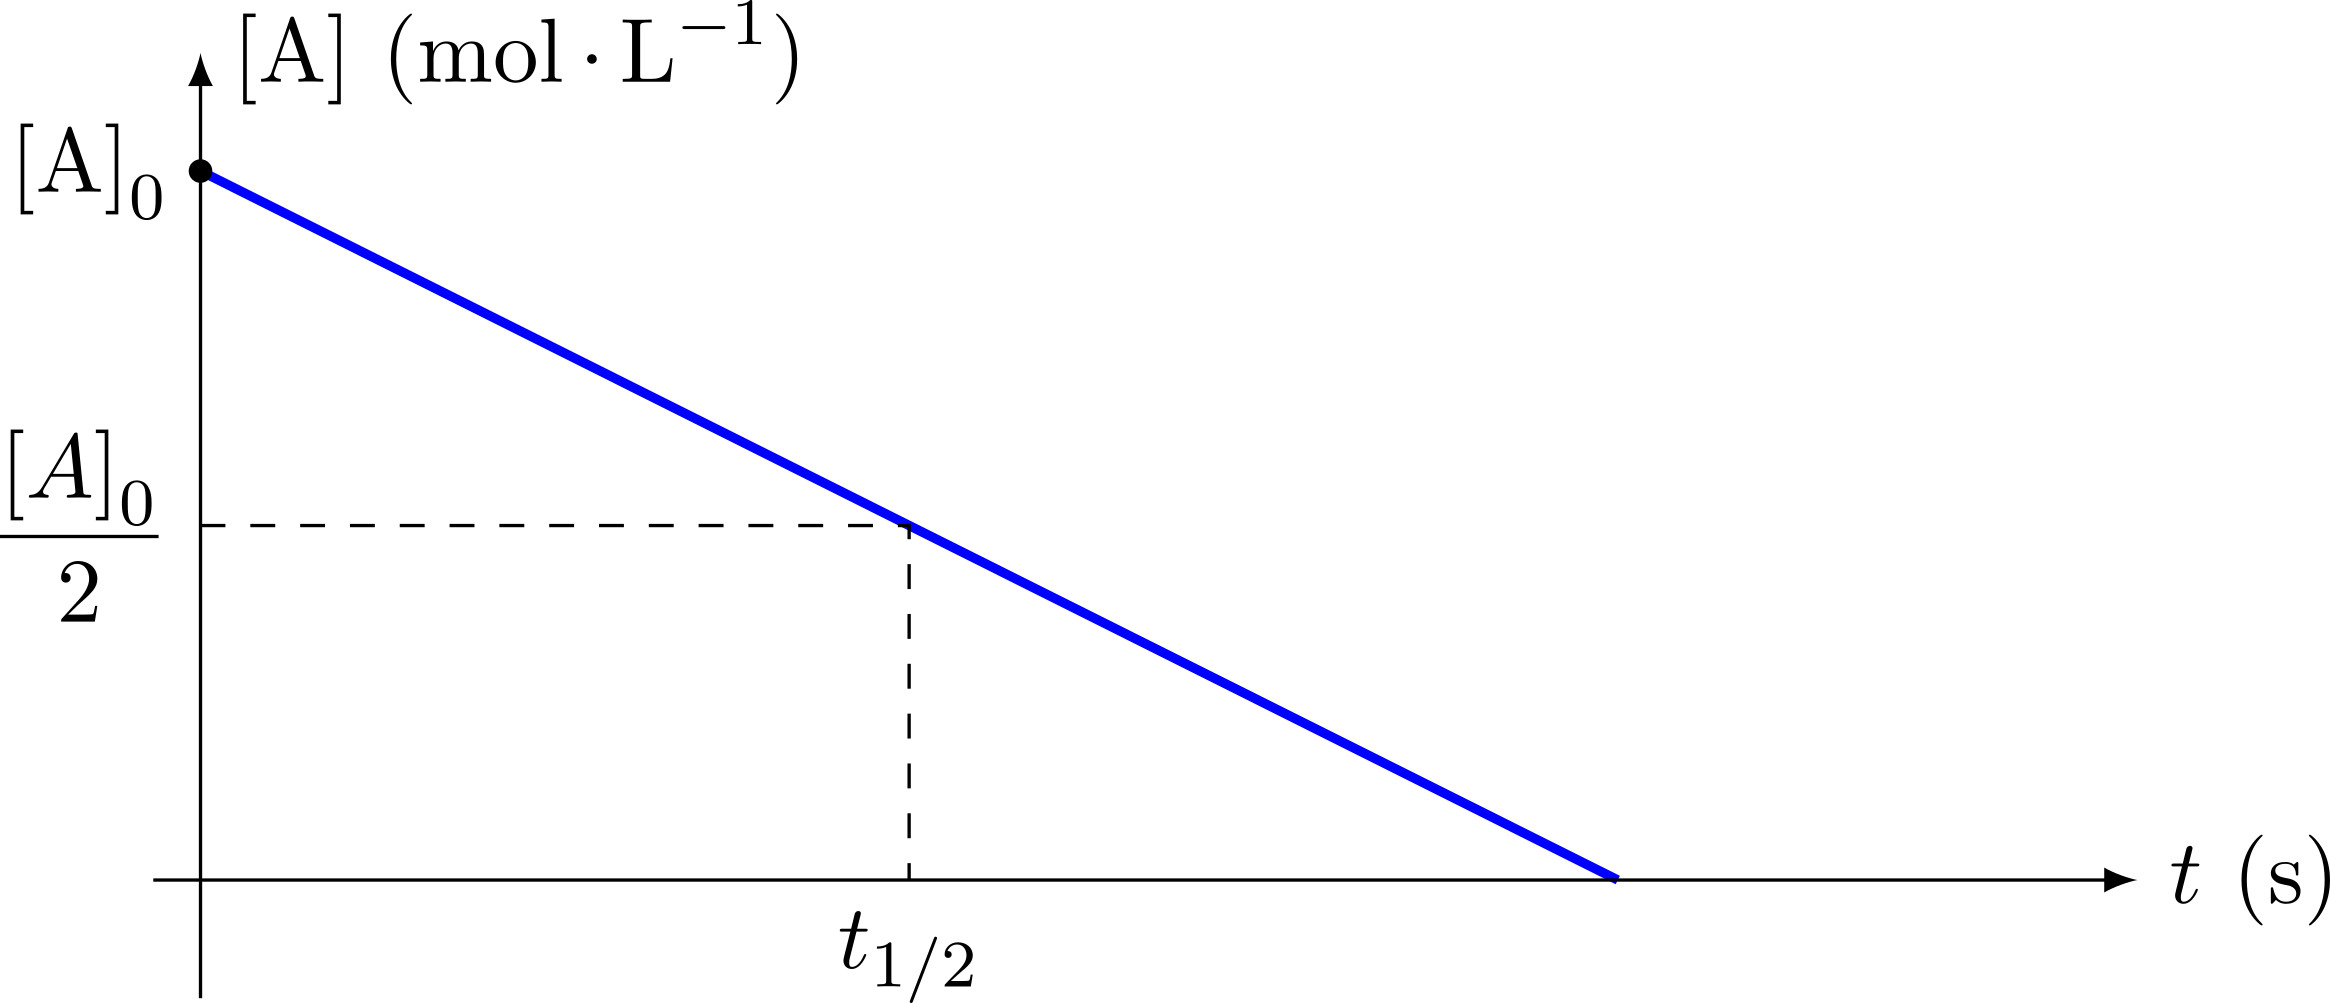
\includegraphics[width=\linewidth, draft=true]{ordre0}
				      }{
					      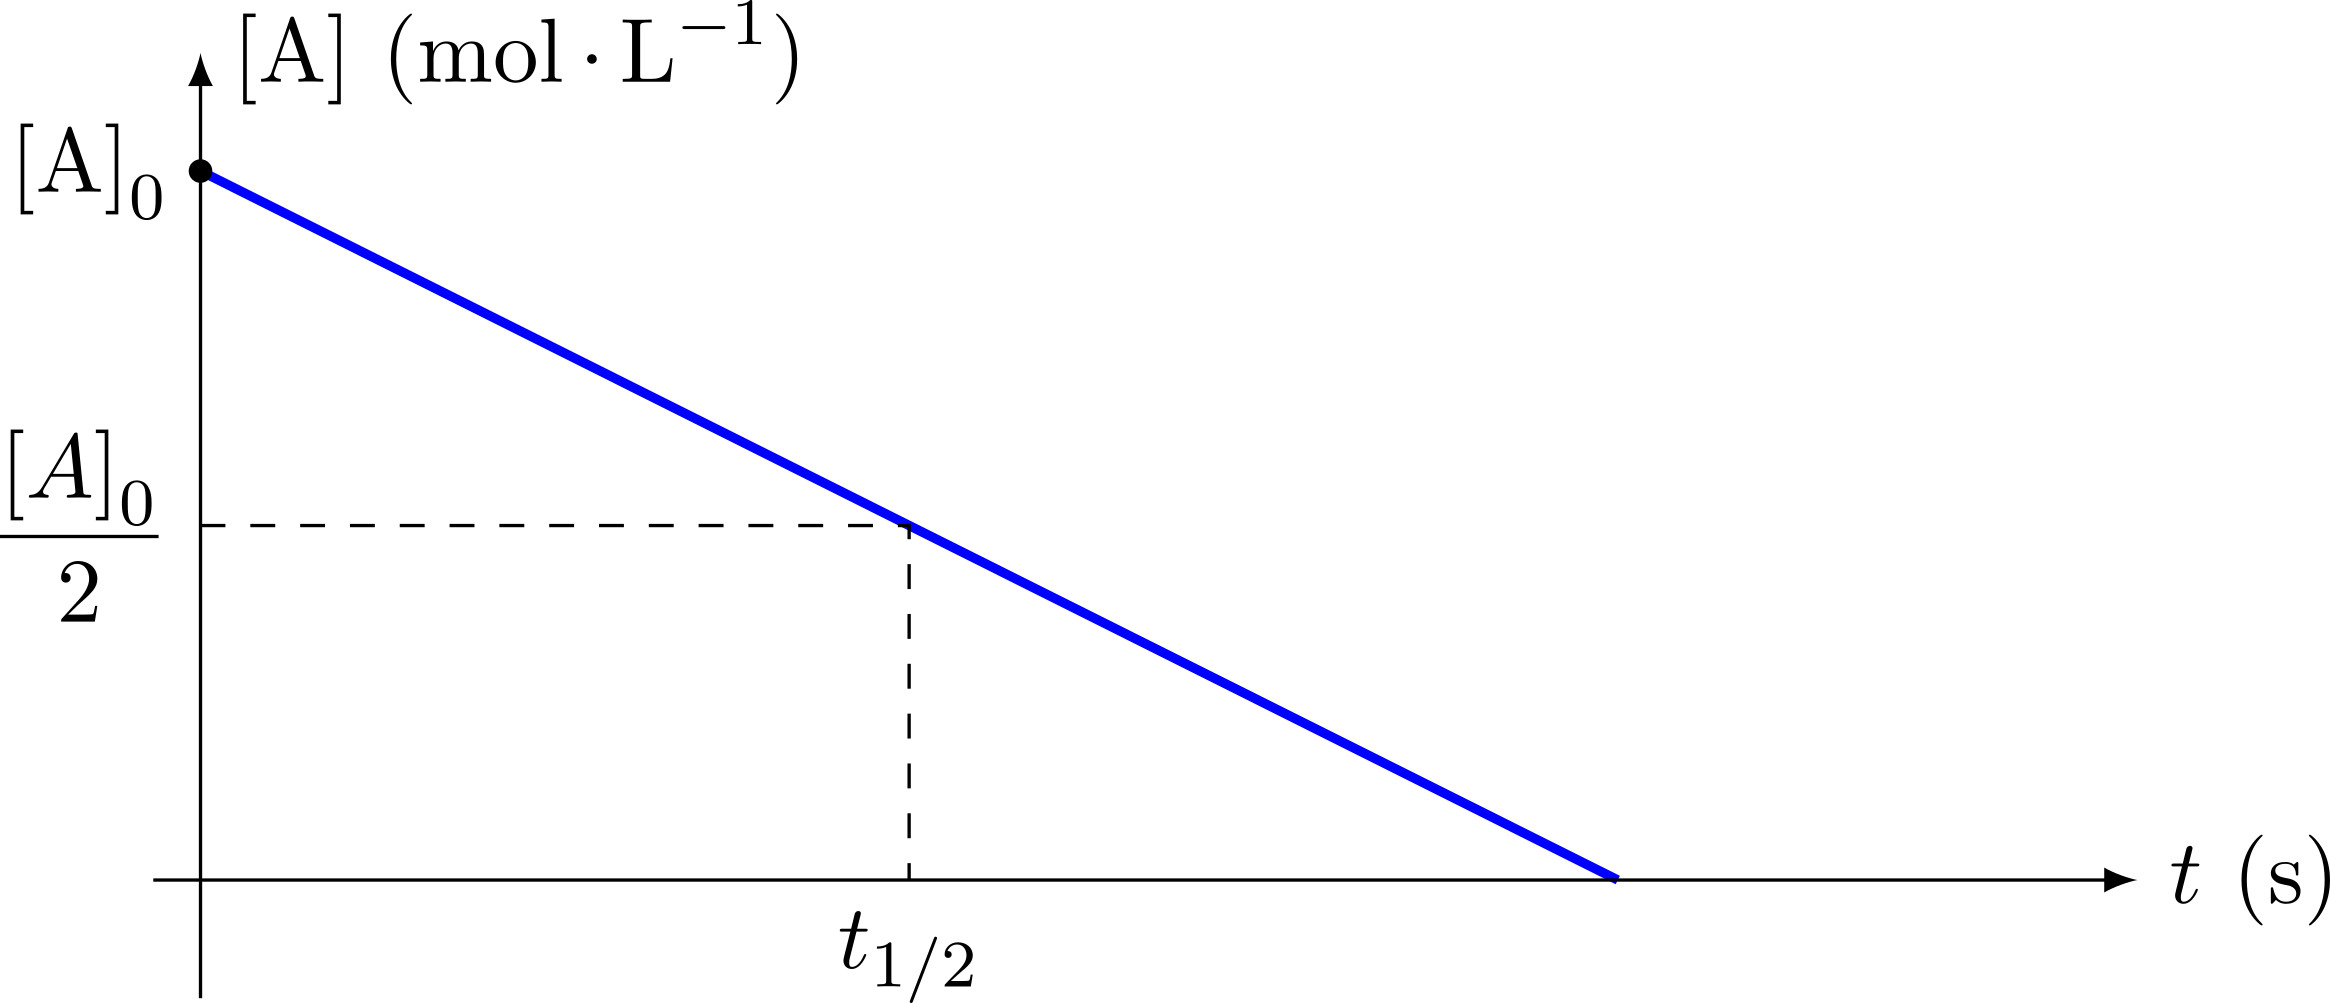
\includegraphics[width=\linewidth]{ordre0}
				      }%
				      \captionof{figure}{Ordre 0}
			      \end{center}
		      \end{isd}
		\item \leftcenters{\textbf{Temps de demi-réaction}~:}{
			      \psw{$\DS t_{1/2} = \frac{[\ce{A}]_0}{2 \abs{\nu_{\ce{A}}} k}$}
		      }
		\item \leftcenters{\textbf{Régression linéaire}~:}{
			      \psw{
				      $y\tikzmark{yn0} =
					      a\tikzmark{an0}x\tikzmark{xn0} + b\tikzmark{bn0}$
				      \tikz[remember picture, overlay]
				      \draw[-stealth, transform canvas={xshift=-6pt, yshift=-6pt}]
				      (pic cs:yn0) --++ (-20pt,-10pt)
				      node[anchor=north] {$[\ce{A}]$}
				      ;
				      \tikz[remember picture, overlay]
				      \draw[-stealth, transform canvas={xshift=-5pt, yshift=-6pt}]
				      (pic cs:an0) --++(-5pt,-10pt)
				      node[anchor=north] {$-\abs{\nu_{\ce{A}}}k$}
				      ;
				      \tikz[remember picture, overlay]
				      \draw[-stealth, transform canvas={xshift=0pt, yshift=-6pt}]
				      (pic cs:xn0) --++(10pt,-10pt)
				      node[anchor=north] {$t$}
				      ;
				      \tikz[remember picture, overlay]
				      \draw[-stealth, transform canvas={xshift=3pt, yshift=-6pt}]
				      (pic cs:bn0) --++(10pt,-10pt)
				      node[anchor=north] {$[\ce{A}]_0$}
				      ;
				      \vspace{20pt}
			      }
		      }
	\end{enumerate}
\end{tcb*}

\begin{tcb*}(demo){Ordre 0}
	\begin{enumerate}[start=3]
		\item[b]{Équation différentielle}:
		      avec le lien entre vitesses (Propriété~\ref{prop:vreacfordisp}), on a
		      \psw{%
			      \[
				      v = \frac{1}{-\abs{\nu_{\ce{A}}}} \dv{[\ce{A}]}{t}
				      \quad \ste{\Longleftrightarrow}{v = k} \quad
				      \boxed{\dv{[\ce{A}]}{t} = - \abs{\nu_{\ce{A}}} k}
			      \]
		      }%
		\item[b]{Résolution}:
		      on intègre directement~:
		      \psw{%
			      \begin{gather*}
				      [\ce{A}](t) - [\ce{A}]_0 = - \abs{\nu_{\ce{A}}}k \cdot t
				      \Lra
				      [\ce{A}](t) = [\ce{A}]_0 - \abs{\nu_{\ce{A}}} k t
			      \end{gather*}
		      }%
	\end{enumerate}
\end{tcb*}

% \subsubsection{Hypothèse}
% \smallbreak
% \leftcenters{%
% 	Avec la loi de vitesse
% }{%
% 	\psw{%
% 		$v = k [{\ce{A}}]^0 = k$
% 	}%
% }
%
% \subsubsection{Unité de $k$}
%
% \psw{%
% L'unité de $k$ \textbf{dans cette situation} est celle de $v$~: c'est donc des
% $\si{mol.L^{-1}.s^{-1}}$.
% }
%
% \subsubsection{Équation différentielle}
% On souhaite déterminer $[{\ce{A}}](t)$. Avec le lien entre vitesse de réaction et
% vitesse de disparition, on a
% \psw{%
% 	\[
% 		\dv{[{\ce{A}}]}{t} = -av
% 		\Lra
% 		\boxed{\dv{[{\ce{A}}]}{t} = -ka}
% 	\]
% }
% \vspace{-15pt}
%
% \subsubsection{Résolution}
% \leftcenters{%
% 	On intègre directement~:
% }{%
% 	\psw{%
% 		$[{\ce{A}}](t) = -kat + K$
% 	}%
% }
% \smallbreak
% \noindent
% avec $K$ une constante à déterminer par condition initiale. Ici, on a simplement
% \psw{%
% 	\begin{gather*}
% 		[{\ce{A}}](0) = [{\ce{A}}]_0 = K
% 		\\\Ra
% 		\boxed{
% 		[{\ce{A}}](t) = [{\ce{A}}]_0 - kat
% 		}%
% 	\end{gather*}
% 	et la concentration diminue \textbf{linéairement avec le temps}.
% }
%
% \begin{center}
% 	\sswitch{
% 		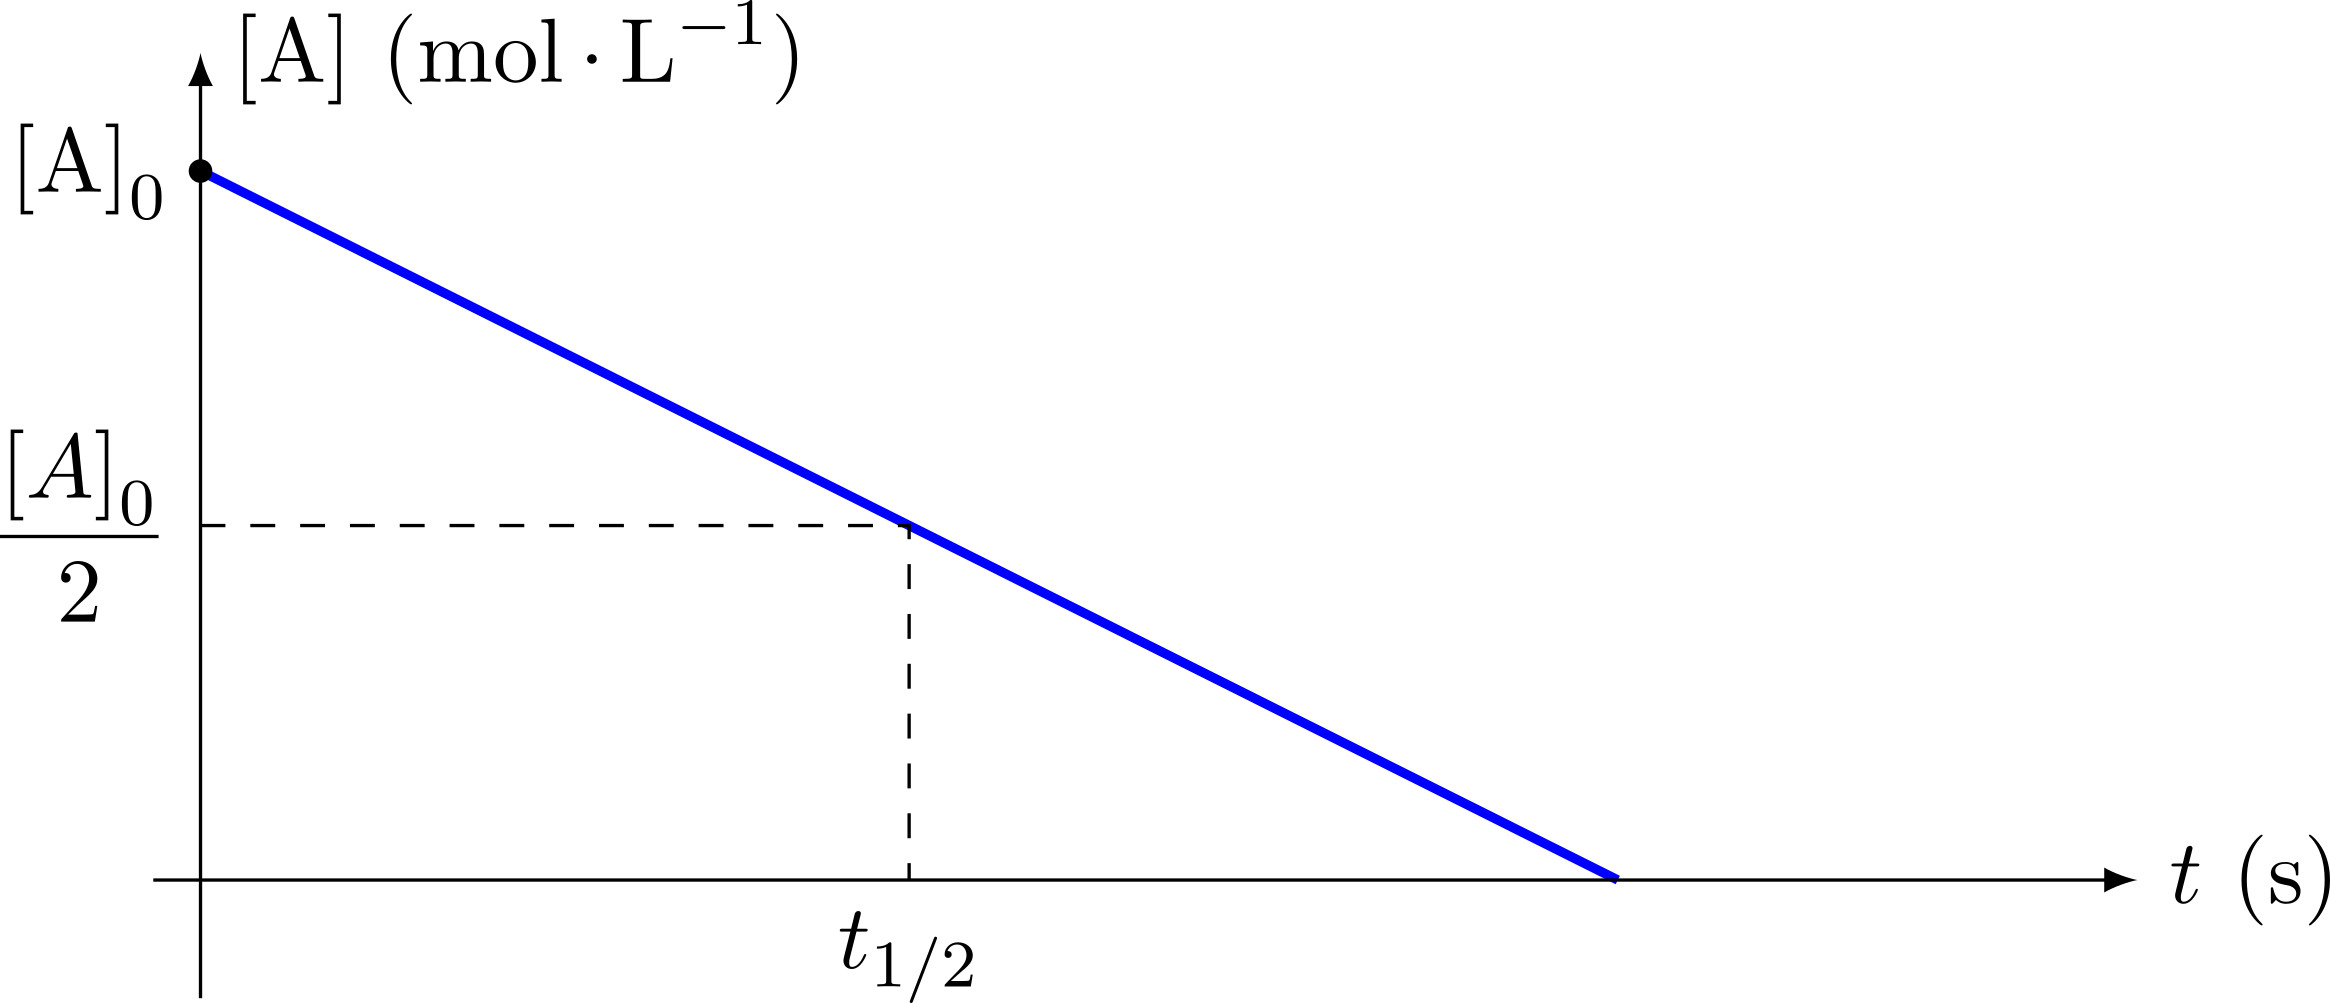
\includegraphics[width=.5\linewidth, draft=true]{ordre0}
% 	}{
% 		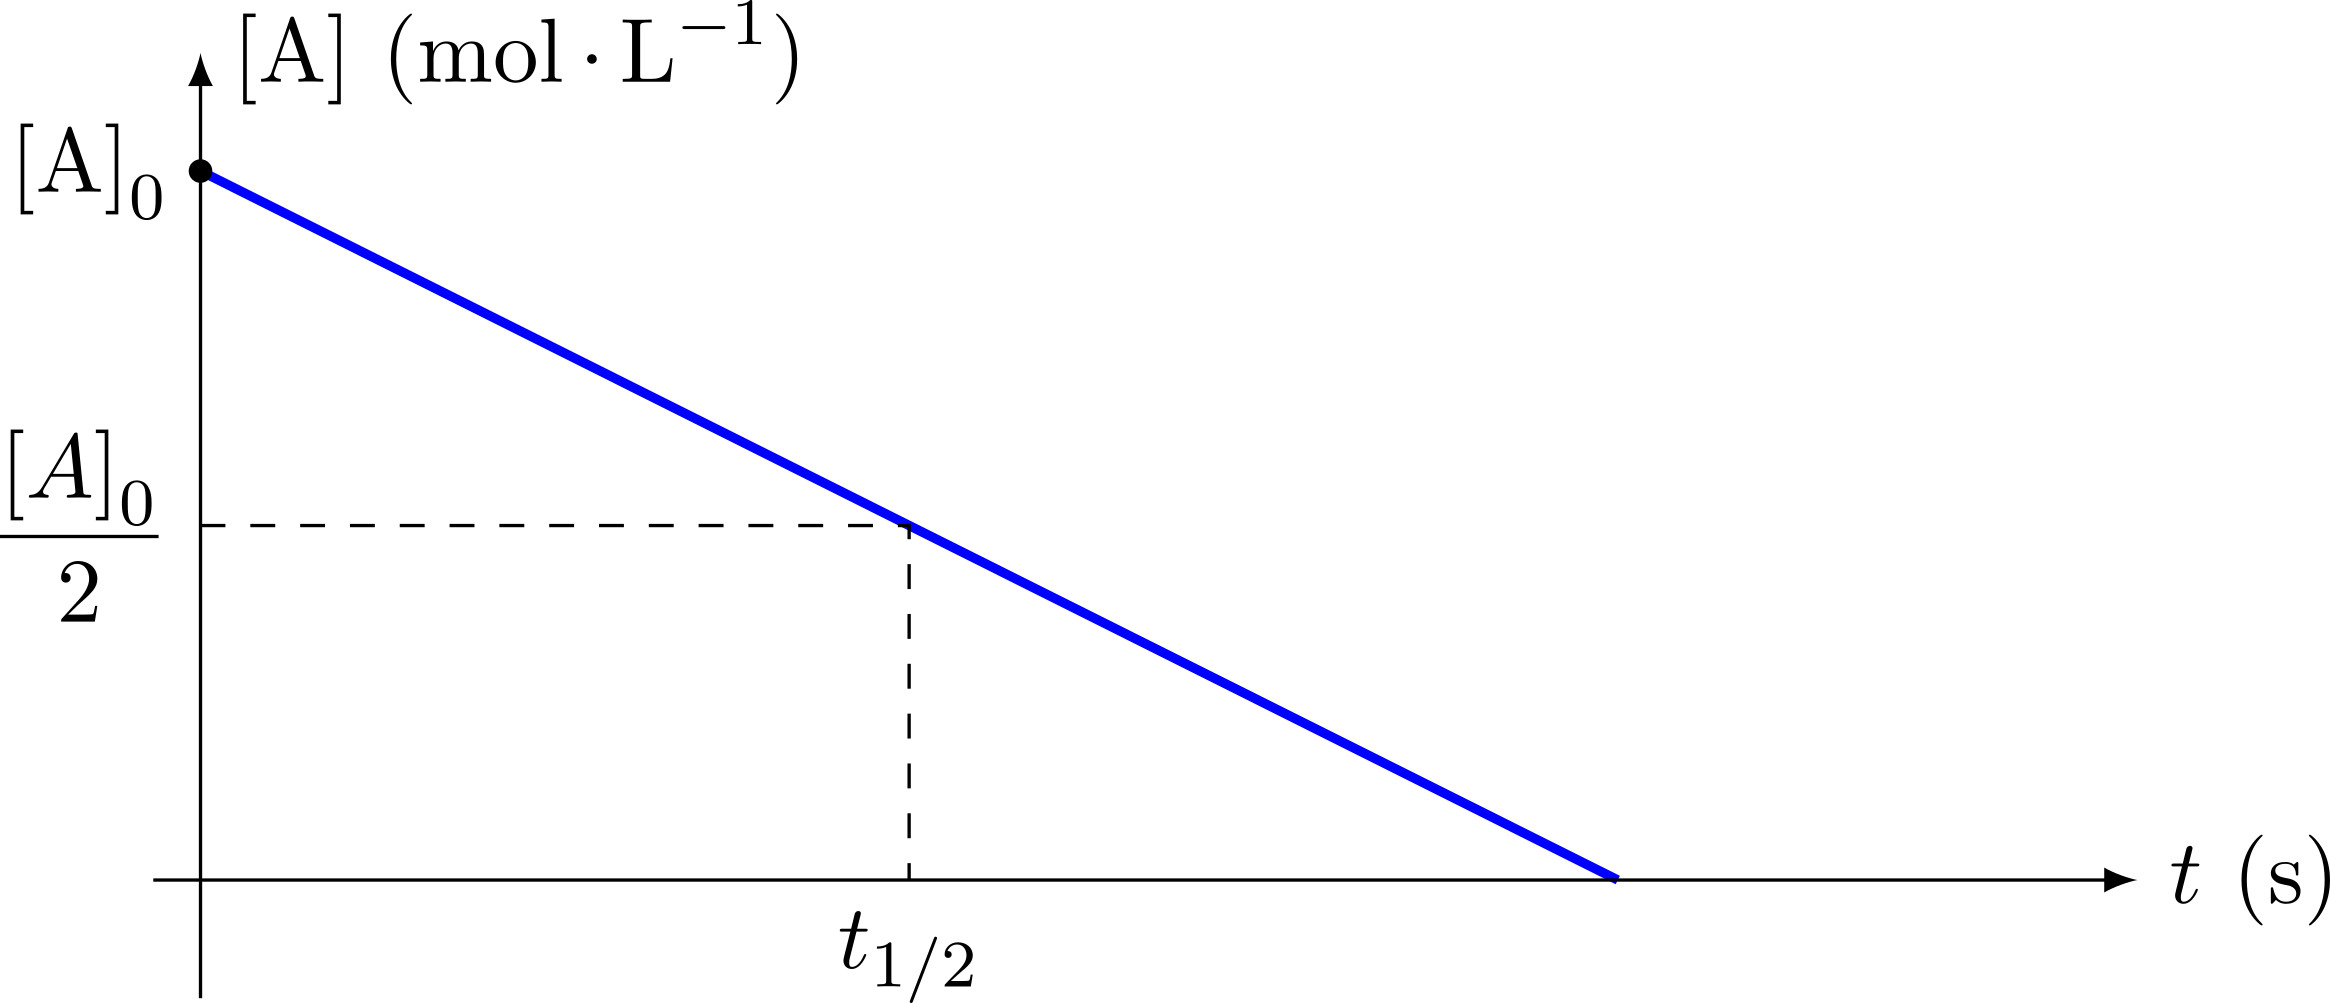
\includegraphics[width=.5\linewidth]{ordre0}
% 	}%
% 	\captionof{figure}{Ordre 0}
% \end{center}
%
% \subsubsection{Temps de demi-réaction}
% Dans le cas où A est le réactif limitant, et donc que sa concentration est nulle
% à la fin de la réaction (comme sur le graphique), on a par définition
% \psw{%
% 	\begin{gather*}
% 		[{\ce{A}}](t_{1/2}) = \frac{[{\ce{A}}]_0}{2}
% 		\Lra
% 		[{\ce{A}}]_0 - kat_{1/2} = \frac{[{\ce{A}}]_0}{2}
% 		\\
% 		\Lra
% 		\boxed{t_{1/2} = \frac{[{\ce{A}}]_0}{2ka}}
% 	\end{gather*}
% }

\begin{tcb}(exem)<lftt>{Ordre 0}
	La décomposition de l'alcool dans le sang suit une telle loi, avec une vitesse
	$v \approx \SI{0.15}{g.L^{-1}.h^{-1}}$ selon l'individu.
\end{tcb}

\subsection{Ordre 1 par rapport à un réactif}

\begin{tcb*}(prop){Ordre 1}
	\begin{enumerate}
		\item \leftcenters{\textbf{Loi de vitesse}~:}{
			      \psw{$v = k [\ce{A}]$}
		      }
		\item \leftcenters{\textbf{Unité}~:}{
			      \psw{$[k] = \frac{[v]}{[\ce{A}]} = \si{s^{-1}}$}
		      }
		\item \leftcenters{\textbf{Équation différentielle}~:}{
		      \psw{$\DS\dv{[\ce{A}]}{t} +\abs{\nu_{\ce{A}}}k [\ce{A}](t) = 0$}
		      }
		\item[b]{Solution et graphique}:
		      \smallbreak
		      \begin{isd}
			      \psw{%
			      \[
				      [\ce{A}](t) = [\ce{A}]_0\exp(-\abs{\nu_{\ce{A}}k t})
			      \]
			      }%
			      \tcblower
			      \begin{center}
				      \sswitch{
					      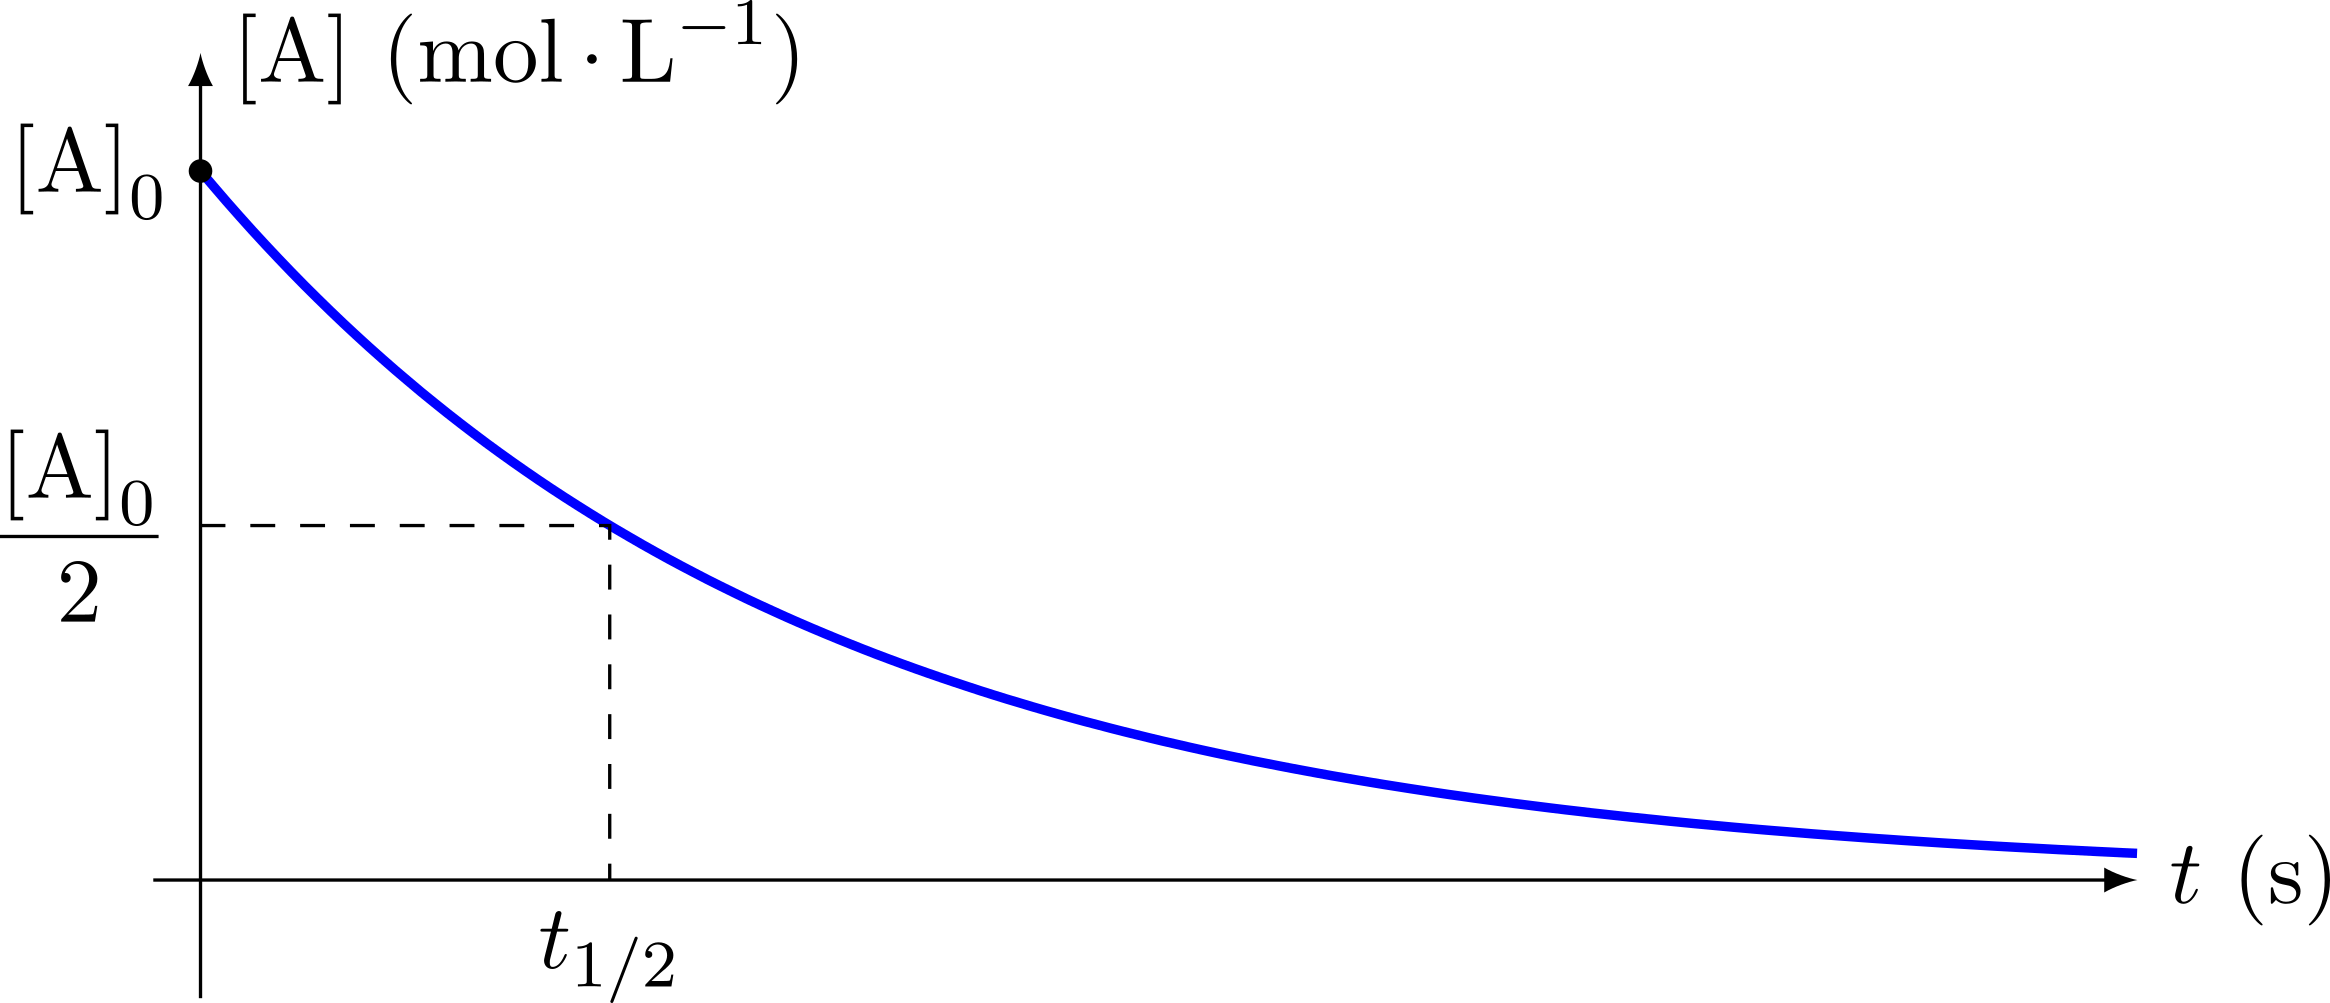
\includegraphics[width=\linewidth, draft=true]{ordre1}
				      }{
					      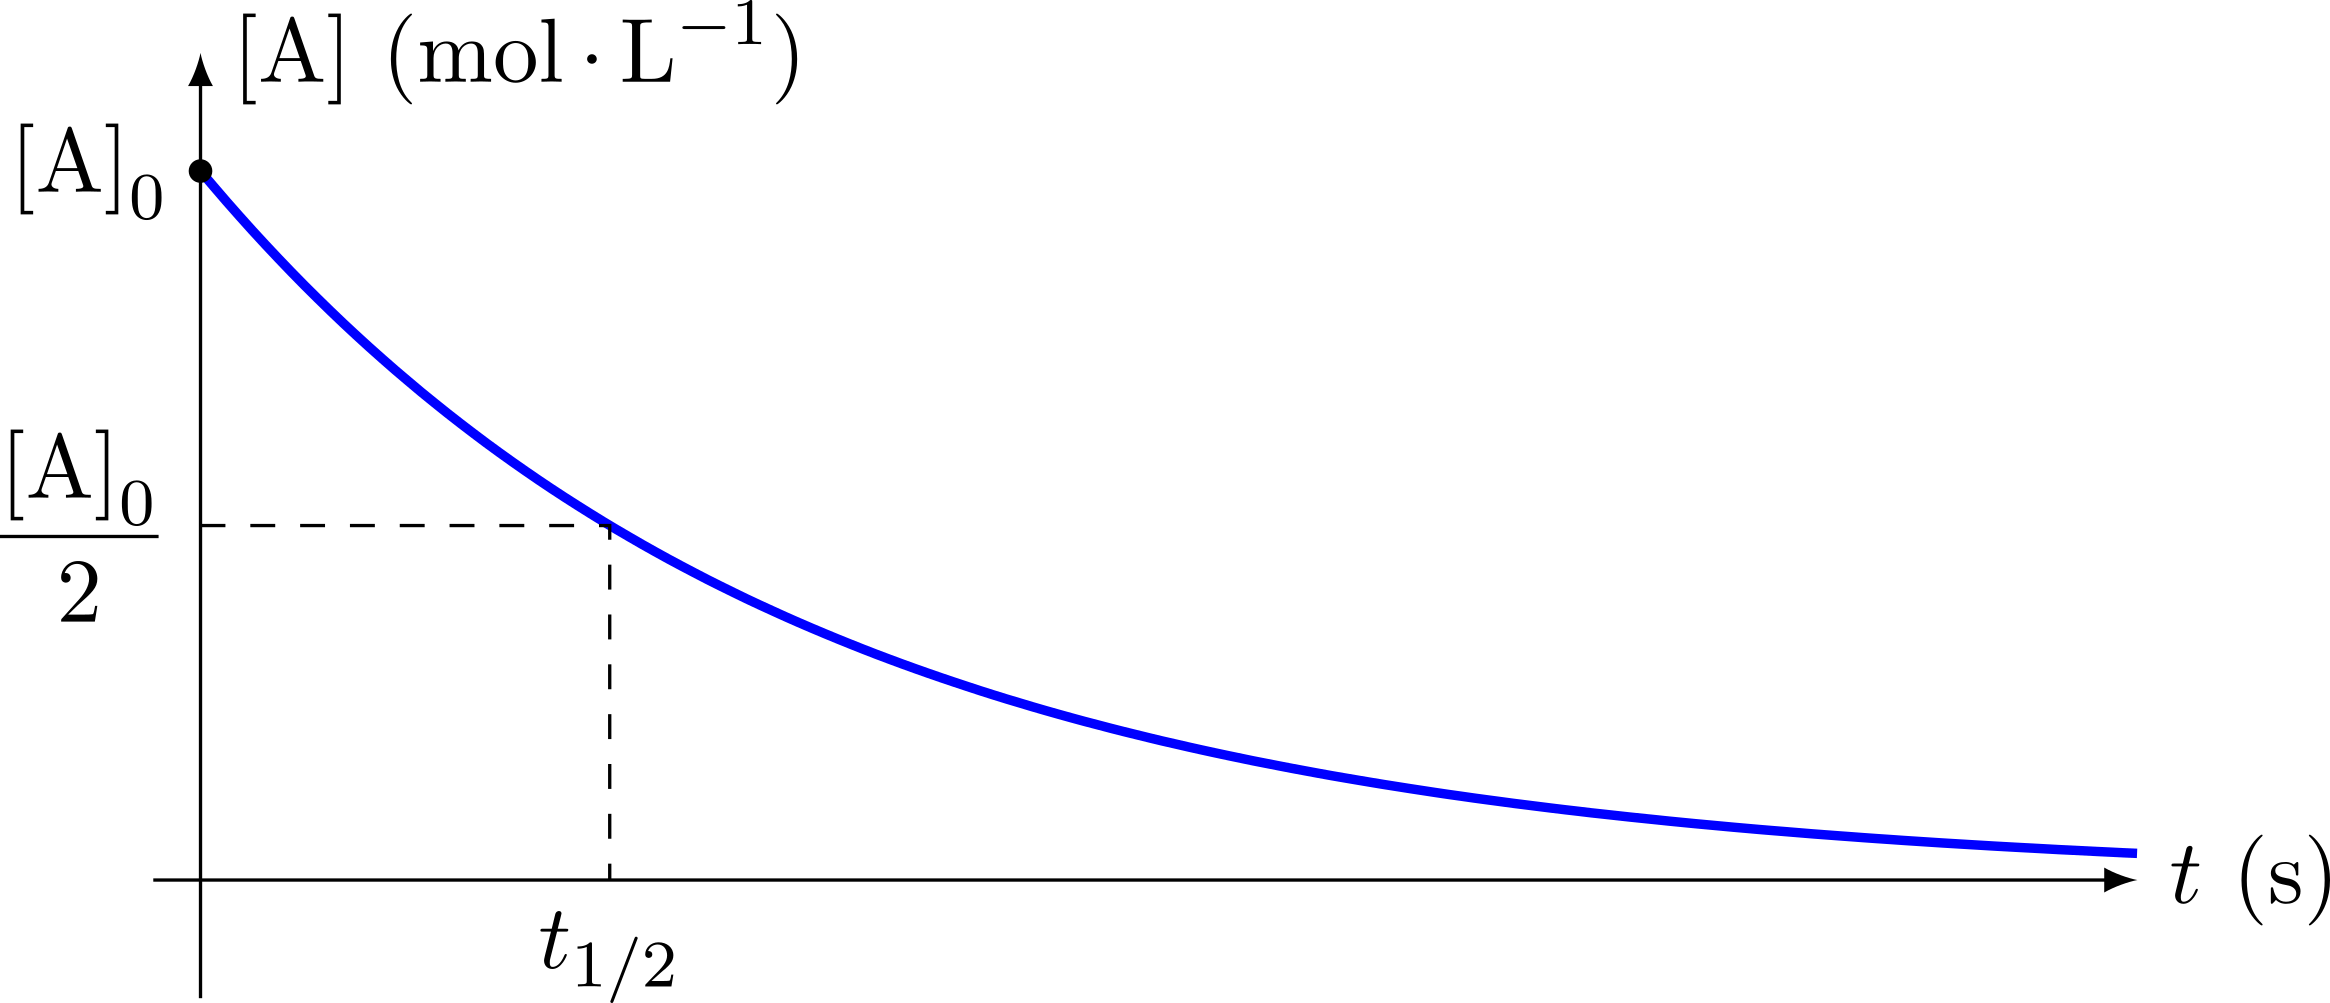
\includegraphics[width=\linewidth]{ordre1}
				      }%
				      \captionof{figure}{Ordre 1}
			      \end{center}
		      \end{isd}
		\item \leftcenters{\textbf{Temps de demi-réaction}~:}{
			      \psw{$\DS t_{1/2} = \frac{\ln 2}{\abs{\nu_{\ce{A}}} k}$}
		      }
		\item \leftcenters{\textbf{Régression linéaire}~:}{
			      \psw{
				      $y\tikzmark{yn1} =
					      a\tikzmark{an1}x\tikzmark{xn1} + b\tikzmark{bn1}$
				      \tikz[remember picture, overlay]
				      \draw[-stealth, transform canvas={xshift=-6pt, yshift=-6pt}]
				      (pic cs:yn1) --++ (-20pt,-10pt)
				      node[anchor=north] {$\ln ([\ce{A}])$}
				      ;
				      \tikz[remember picture, overlay]
				      \draw[-stealth, transform canvas={xshift=-5pt, yshift=-6pt}]
				      (pic cs:an1) --++(-5pt,-10pt)
				      node[anchor=north] {$-\abs{\nu_{\ce{A}}}k$}
				      ;
				      \tikz[remember picture, overlay]
				      \draw[-stealth, transform canvas={xshift=0pt, yshift=-6pt}]
				      (pic cs:xn1) --++(10pt,-10pt)
				      node[anchor=north] {$t$}
				      ;
				      \tikz[remember picture, overlay]
				      \draw[-stealth, transform canvas={xshift=3pt, yshift=-6pt}]
				      (pic cs:bn1) --++(20pt,-10pt)
				      node[anchor=north] {$\ln ([\ce{A}]_0)$}
				      ;
				      \vspace{20pt}
			      }
		      }
	\end{enumerate}
\end{tcb*}

\begin{tcb*}(demo){Ordre 1}
	\begin{enumerate}[start=3]
		\item[b]{Équation différentielle}:
		      avec le lien entre vitesses (Propriété~\ref{prop:vreacfordisp}), on a
		      \psw{%
			      \[
				      v = \frac{1}{-\abs{\nu_{\ce{A}}}} \dv{[\ce{A}]}{t}
				      \quad \ste{\Longleftrightarrow}{v = k[\ce{A}]} \quad
				      \boxed{\dv{[\ce{A}]}{t} + \abs{\nu_{\ce{A}}} k [\ce{A}] = 0}
			      \]
		      }%
		\item[b]{Résolution}:
		      On résout en injectant $[\ce{A}](t) = K\exr^{-rt}$ puis en utilisant la
		      condition initiale~:
		      \psw{%
			      \begin{gather*}
				      [\ce{A}](t) = K\exr^{-\abs{\nu_{\ce{A}}}kt}
				      \quad \stc{\Longrightarrow}{CI} \quad
				      [\ce{A}](t) = [\ce{A}]_0\exr^{-\abs{\nu_{\ce{A}}}kt}
			      \end{gather*}
		      }%
	\end{enumerate}
\end{tcb*}

% \subsubsection{Hypothèse}
% \leftcenters{%
% Soit la réaction
% }{%
% $
% 	a{\ce{A}} + b{\ce{B}}
% 	=
% 	c{\ce{C}} +d{\ce{D}}
% $
% }
% \smallbreak
% \leftcenters{%
% 	Avec la loi de vitesse
% }{%
% 	\psw{%
% 		$v = k [{\ce{A}}]$
% 	}%
% }
%
% \subsubsection{Unité de $k$}
%
% \psw{%
% 	L'unité de $k$ \textbf{dans cette situation} est celle de $v$ divisée par celle
% 	d'une concentration~: c'est donc des $\si{s^{-1}}$.
% }
%
% \subsubsection{Équation différentielle}
% On souhaite déterminer $[{\ce{A}}](t)$. Avec le lien entre vitesse de réaction et
% vitesse de disparition, on a
% \psw{%
% 	\begin{gather*}
% 		\dv{[{\ce{A}}]}{t} = -av \Lra \dv{[{\ce{A}}]}{t} = -ka[{\ce{A}}]
% 		\\\Lra
% 		\boxed{\dv{[{\ce{A}}]}{t} + ka[{\ce{A}}] = 0}
% 	\end{gather*}
% }
% \vspace{-15pt}
%
% \subsubsection{Résolution}
% La solution générale de cette équation du premier degré est
% \psw{%
% 	\[[{\ce{A}}](t) = K\exp(-kat)\]
% }
% avec $K$ une constante à déterminer par condition initiale. Ici, on a simplement
% \psw{%
% 	\begin{gather*}
% 		[{\ce{A}}](0) = [{\ce{A}}]_0 = K
% 		\\\Ra
% 		\boxed{[{\ce{A}}](t) = [{\ce{A}}]_0\exp(-kat)}
% 	\end{gather*}
% 	et la concentration diminue \textbf{exponentiellement avec le temps}. C'est le
% 	cas le plus fréquent.
% }
%
% \begin{center}
% 	\sswitch{
% 		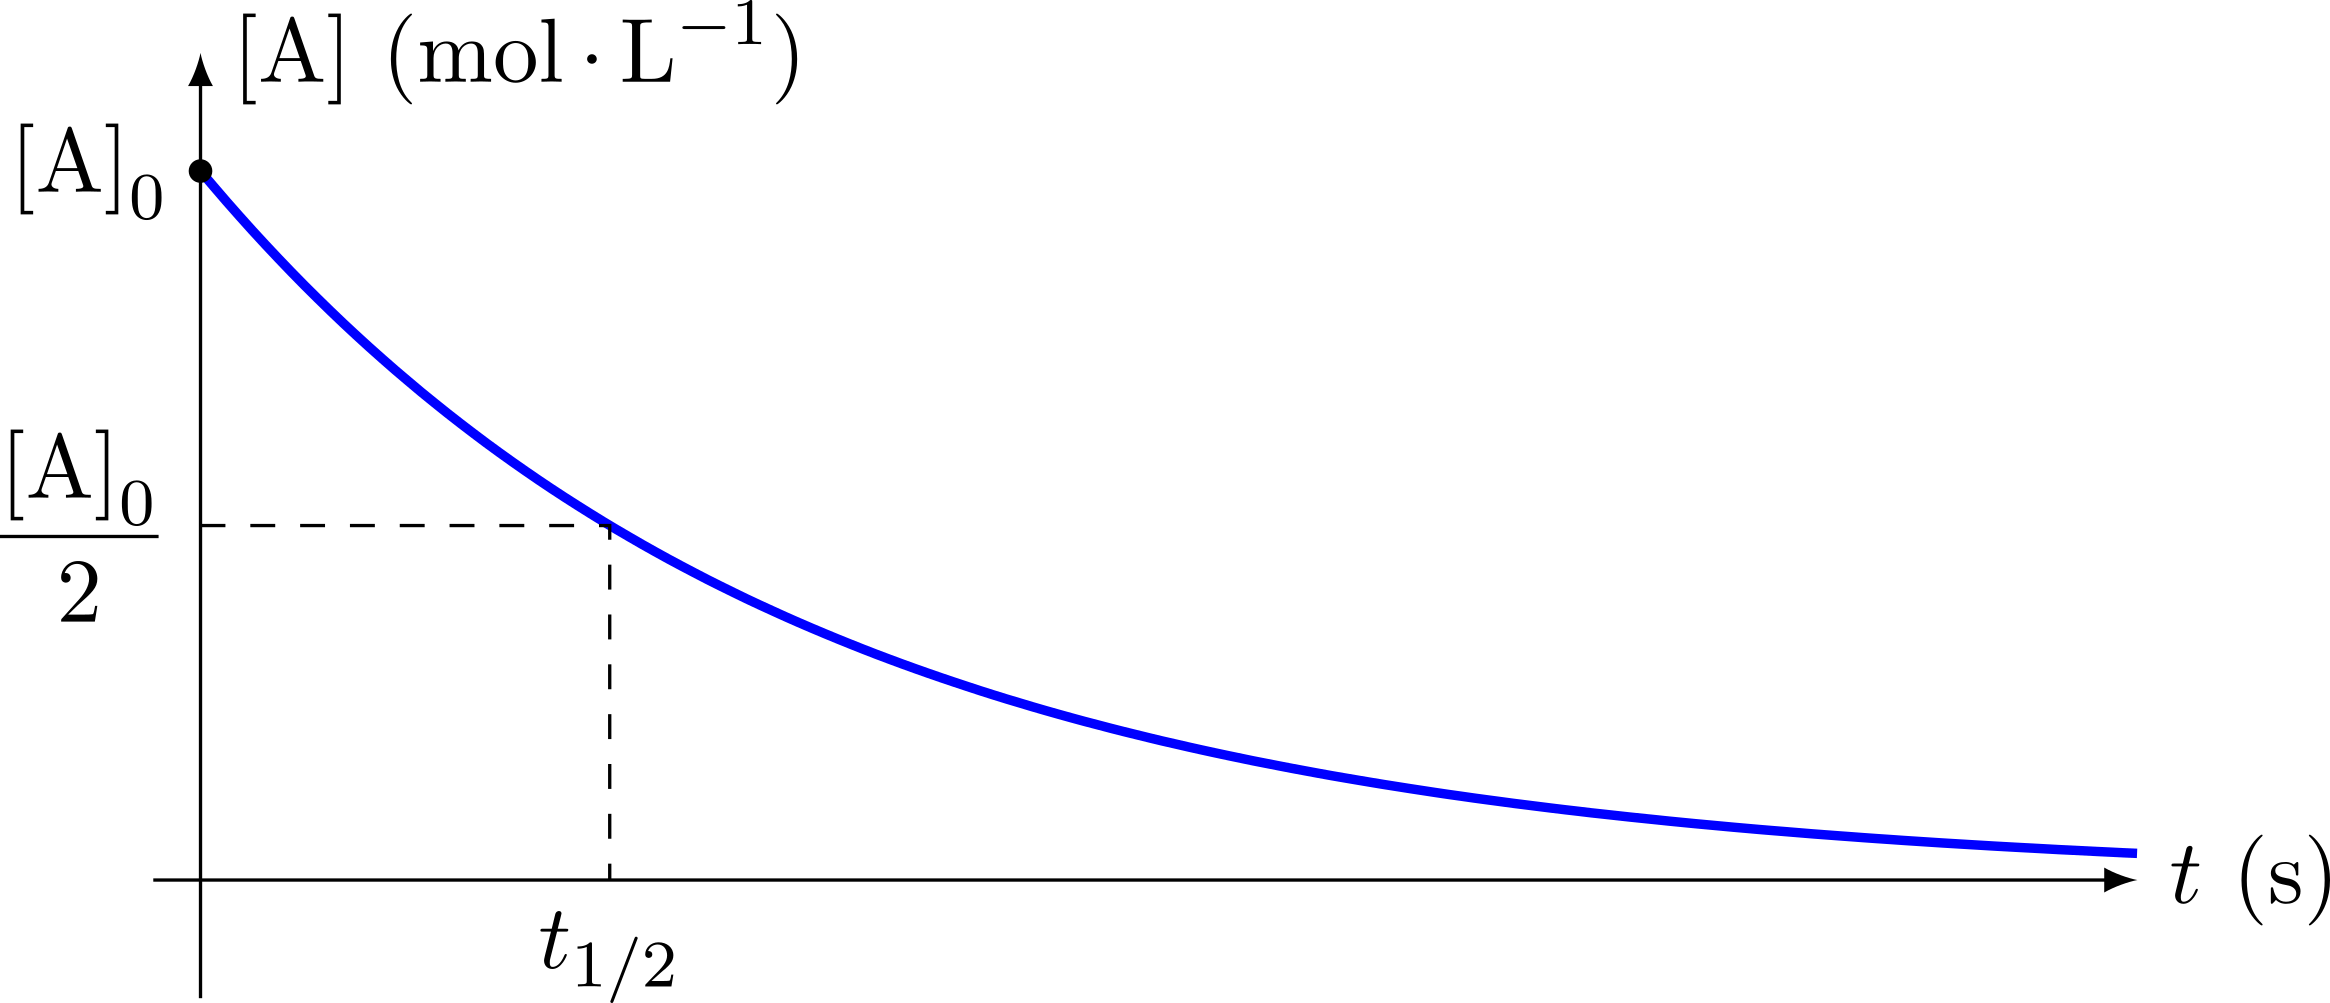
\includegraphics[width=.5\linewidth, draft=true]{ordre1}
% 	}{
% 		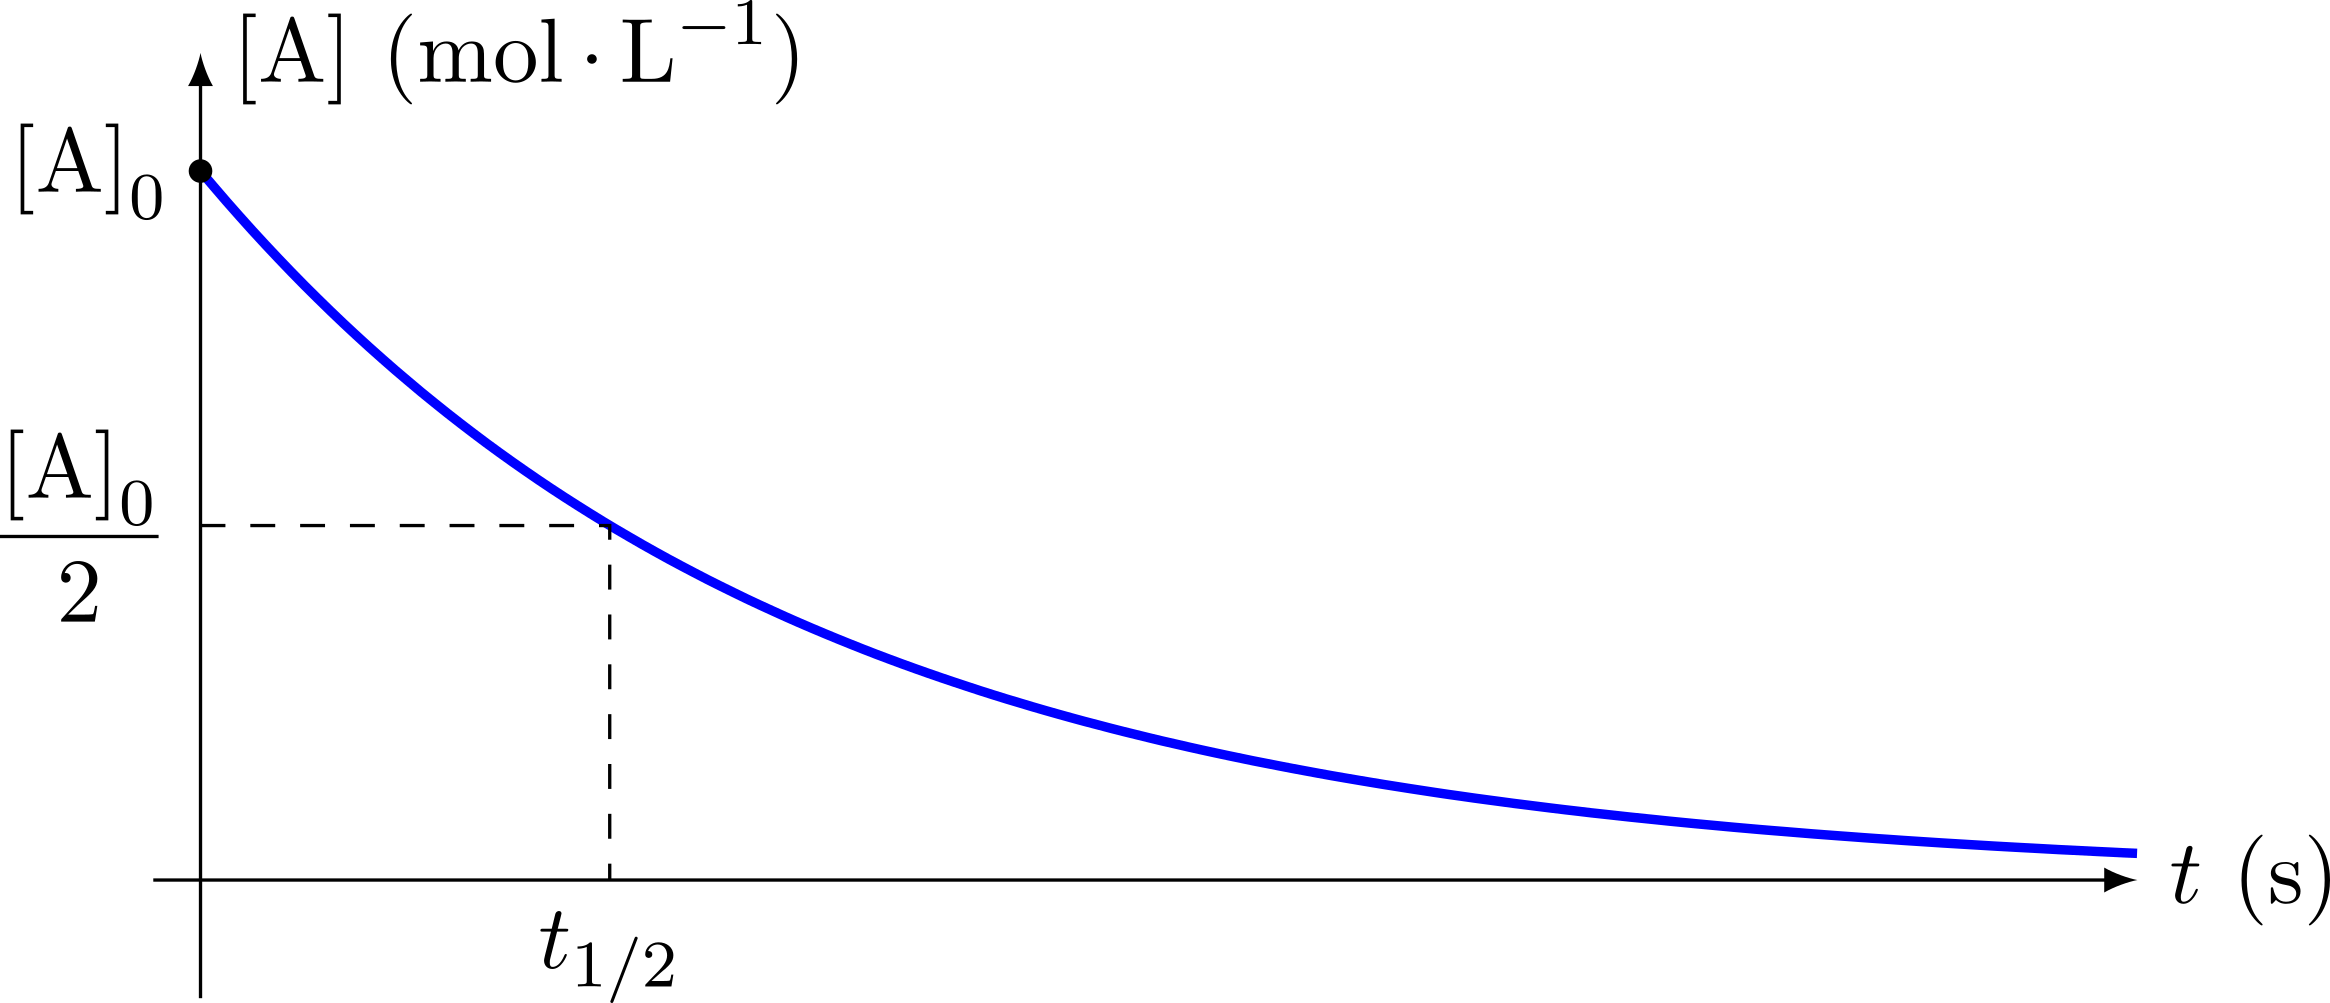
\includegraphics[width=.5\linewidth]{ordre1}
% 	}%
% 	\captionof{figure}{Ordre 1}
% \end{center}
%
% \subsubsection{Temps de demi-réaction}
% Dans le cas où A est le réactif limitant, et donc que sa concentration est nulle
% à la fin de la réaction (comme sur le graphique), on a par définition
% \psw{%
% 	\begin{gather*}
% 		[{\ce{A}}](t_{1/2}) = \frac{[{\ce{A}}]_0}{2}
% 		\Lra
% 		[{\ce{A}}]_0\exp(-kat_{1/2}) = \frac{[{\ce{A}}]_0}{2}\\
% 		\Lra
% 		-kat_{1/2} = \ln \left( \frac{1}{2} \right) = -\ln 2\\
% 		\Lra
% 		\boxed{t_{1/2} = \frac{\ln 2}{ka}}
% 	\end{gather*}
% }
% \vspace{-15pt}

\begin{tcb}[breakable](exem)<lftt>{Ordre 1}
	La désintégration du carbone 14 (et tous les éléments radioactifs) suit une
	cinétique d'ordre 1.
	\smallbreak
	Le principe de datation au carbone 14 est que pendant la
	vie d'un organisme vivant, la proportion qu'il contient est égale à celle de
	l'atmosphère par équilibre~; à sa mort, l'équilibre est rompu et le carbone se
	désintègre.
	\smallbreak
	La demi-vie du ${\ce{^{14}C}}$ étant de
	\SI{5730}{ans}, on peut mesurer la quantité de carbone 14 et donc l'âge d'un
	échantillon jusqu'à environ \SI{50000}{ans}.
\end{tcb}

\subsection{Ordre 2 par rapport à un réactif}
\begin{tcb*}(prop){Ordre 2}
	\begin{enumerate}
		\item \leftcenters{\textbf{Loi de vitesse}~:}{
			      \psw{$v = k [\ce{A}]^2$}
		      }
		\item \leftcenters{\textbf{Unité}~:}{
		      \psw{$[k] = \frac{[v]}{[\ce{A}]^2} = \si{mol^{-1}.L^{-1}.s^{-1}}$}
		      }
		\item \leftcenters{\textbf{Équation différentielle}~:}{
		      \psw{$\DS\dv{[\ce{A}]}{t} = -\abs{\nu_{\ce{A}}}k [\ce{A}]^2$}
		      }
		\item[b]{Solution et graphique}:
		      \smallbreak
		      \begin{isd}
			      \psw{%
				      \[
					      \frac{1}{[\ce{A}](t)} = \frac{1}{[\ce{A}]_0} + \abs{\nu_{\ce{A}}}k t
				      \]
			      }%
			      \tcblower
			      \begin{center}
				      \sswitch{
					      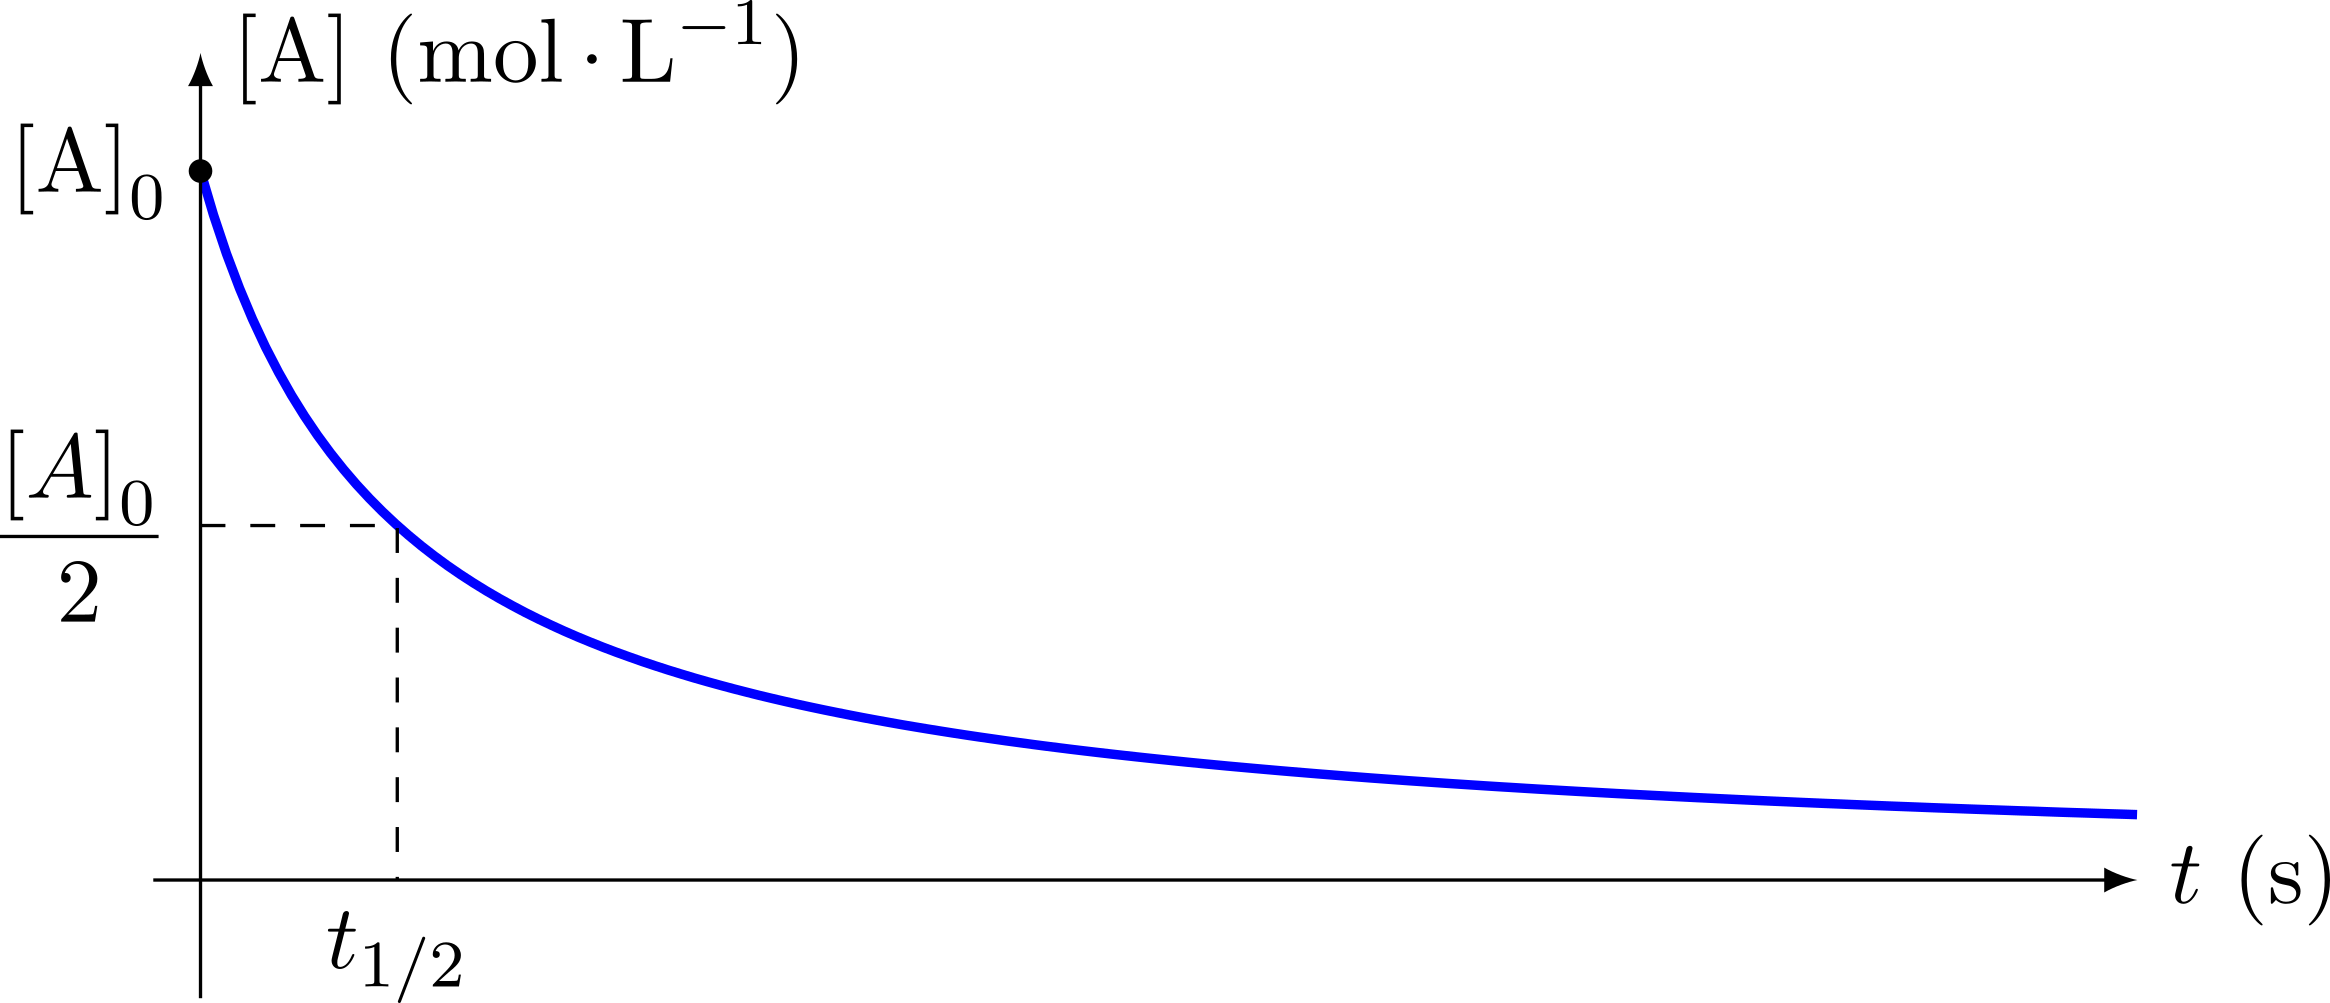
\includegraphics[width=\linewidth, draft=true]{ordre2}
				      }{
					      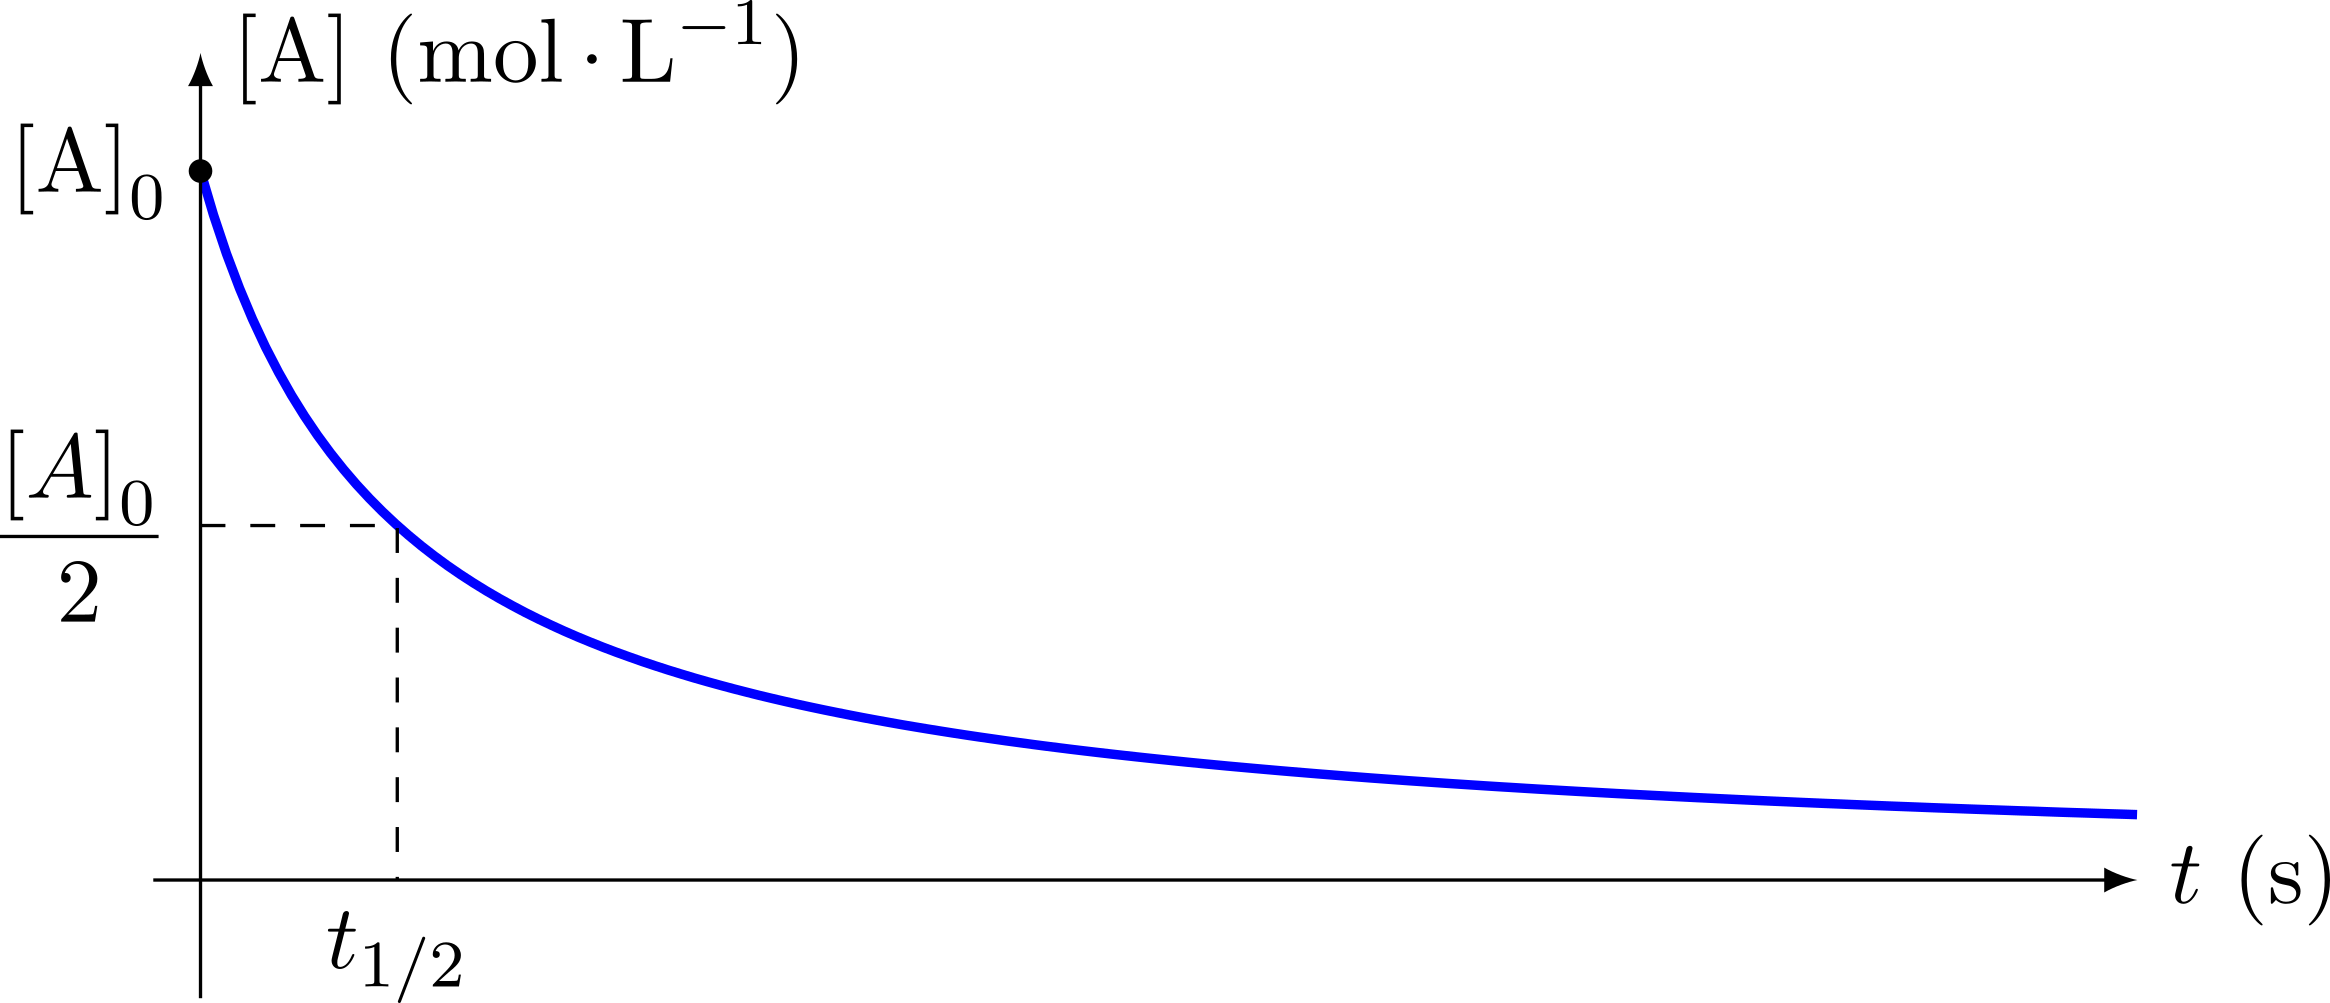
\includegraphics[width=\linewidth]{ordre2}
				      }%
				      \captionof{figure}{Ordre 2}
			      \end{center}
		      \end{isd}
		\item \leftcenters{\textbf{Temps de demi-réaction}~:}{
			      \psw{$\DS t_{1/2} = \frac{1}{\abs{\nu_{\ce{A}}} k [\ce{A}]_0}$}
		      }
		\item \leftcenters{\textbf{Régression linéaire}~:}{
			      \psw{
				      $y\tikzmark{yn2} =
					      a\tikzmark{an2}x\tikzmark{xn2} + b\tikzmark{bn2}$
				      \tikz[remember picture, overlay]
				      \draw[-stealth, transform canvas={xshift=-6pt, yshift=-6pt}]
				      (pic cs:yn2) --++ (-20pt,-10pt)
				      node[anchor=north] {$\frac{1}{[\ce{A}]}$}
				      ;
				      \tikz[remember picture, overlay]
				      \draw[-stealth, transform canvas={xshift=-5pt, yshift=-6pt}]
				      (pic cs:an2) --++(-5pt,-10pt)
				      node[anchor=north] {$+\abs{\nu_{\ce{A}}}k$}
				      ;
				      \tikz[remember picture, overlay]
				      \draw[-stealth, transform canvas={xshift=0pt, yshift=-6pt}]
				      (pic cs:xn2) --++(10pt,-10pt)
				      node[anchor=north] {$t$}
				      ;
				      \tikz[remember picture, overlay]
				      \draw[-stealth, transform canvas={xshift=3pt, yshift=-6pt}]
				      (pic cs:bn2) --++(10pt,-10pt)
				      node[anchor=north] {$\frac{1}{[\ce{A}]_0}$}
				      ;
				      \vspace{20pt}
			      }
		      }
	\end{enumerate}
\end{tcb*}

Dans ce cas, l'équation différentielle est \textbf{non-linéaire}. Il faut ruser
pour la résoudre.

\begin{tcb*}[breakable, sidebyside](tool){Séparation des variables}
	En mathématiques, la séparation des variables est une méthode clé de
	résolution d'équations différentielles, très utilisée en physique à plusieurs
	variables et dans le cas des équations non-linéaires.
	\smallbreak
	Soient $f(x)$ et $g(x)$ des fonctions de la variable $x$, et $h$ une fonction
	de la «~variable~» $f(x)$. On peut effectuer un changement de variable $y =
		f(x)$, et isoler les dépendances en $x$ et en $y$~:
	\tcblower
	\psw{%
		\begin{DispWithArrows*}[fleqn, mathindent=-5pt]
			\dv{f}{x} &= g (x) \cdot h (f (x))
			\Arrow{$y = f(x)$}
			\\\Lra
			\dv{y}{x} &= g(x) \cdot h(y)
			\Arrow{Séparation}
			\\\Lra
			\frac{\dd{y}}{h(y)} &= g (x) \dd{x}
			\Arrow{Intégra$^\circ$ séparée}
			\\\Ra
			\Aboxed{\int_{y} \frac{y}{h(y)} &= \int_{x} g(x) \dd{x}}
		\end{DispWithArrows*}
	}%
\end{tcb*}

\begin{tcb*}(demo){Ordre 2}
	\begin{enumerate}[start=3]
		\item[b]{Équation différentielle}:
		      avec le lien entre vitesses (Propriété~\ref{prop:vreacfordisp}), on a
		      \psw{%
			      \[
				      v = \frac{1}{-\abs{\nu_{\ce{A}}}} \dv{[\ce{A}]}{t}
				      \quad \ste{\Longleftrightarrow}{v = k[\ce{A}]^2} \quad
				      \boxed{\dv{[\ce{A}]}{t} = -\abs{\nu_{\ce{A}}} k [\ce{A}]^2}
			      \]
		      }%
		\item[b]{Résolution}:
		      on \textbf{sépare les variables} et on utilise la dérivée de la
		      fonction inverse~:
		      \psw{%
			      \begin{DispWithArrows*}
				      % \dv{[{\ce{A}}]}{t} &= -\abs{\nu_{\ce{A}}}k[{\ce{A}}]^2
				      % \Arrow{Séparation des variables}
				      % \\\Lra
				      - \frac{\dd{[\ce{A}]}}{[{\ce{A}}]^2} &= \abs{\nu_{\ce{A}}}k \dd{t}
				      \CArrow{$\DS\int$}
				      \\\Lra
				      \int_{[\ce{A}]_0}^{[\ce{A}]} -\frac{\dd{[\ce{A}]}}{[{\ce{A}}]^2}
				      &=
				      \int_{t=0}^{t} \abs{\nu_{\ce{A}}}k \dd{t}
				      \Arrow{$\DS\left( \frac{1}{f} \right)' = - \frac{f'}{f^2}$}
				      \\\Lra
				      \int_{[\ce{A}]_0}^{[\ce{A}](t)}
				      \dd{\left( \frac{1}{[\ce{A}](t)} \right)}
				      &=
				      \abs{\nu_{\ce{A}}}k \cdot \int_{t=0}^{t} \dd{t}
				      \Arrow{$\int_a^b \dd{(\cdot )} = [(\cdot )]_a^b$}
				      \\\Lra
				      \frac{1}{[{\ce{A}}]} - \frac{1}{[\ce{A}]_0} &= \abs{\nu_{\ce{A}}}k \cdot t
				      \\\Lra
				      \Aboxed{\frac{1}{[{\ce{A}}]} &= \frac{1}{[\ce{A}]_0} + \abs{\nu_{\ce{A}}}kt}
			      \end{DispWithArrows*}
		      }%
		\item[b]{Temps de demi-réaction}: par définition, $[\ce{A}](t_{1/2}) =
			      \frac{[\ce{A}]_0}{2}$, soit~:
		      \psw{%
			      \begin{gather*}
				      \frac{1}{[\ce{A}](t_{1/2})} = \frac{2}{[\ce{A}]_0} =
				      \frac{1}{[\ce{A}]_0} + \abs{\nu_{\ce{A}}}k \cdot t_{1/2}
				      \Lra
				      \boxed{t_{1/2} = \frac{1}{\abs{\nu_{\ce{A}}}k \cdot [\ce{A}]_0}}
			      \end{gather*}
		      }%
		      % On peut également écrire
		      % \[
		      %  \psw{%
		      %  \boxed{%
		      %   [{\ce{A}}](t) =
		      %   \frac{1}{\frac{1}{[{\ce{A}}]_0} + \abs{\nu_{\ce{A}}}kt}
		      %  }%
		      %  \Lra
		      %  \boxed{%
		      %  [{\ce{A}}](t) =
		      %  \frac{[{\ce{A}}]_0}{1 + \abs{\nu_{\ce{A}}}kt[{\ce{A}}]_0}
		      %  }%
		      %  }%
		      % \]
	\end{enumerate}
\end{tcb*}

% \subsubsection{Hypothèse}
% \leftcenters{%
% Soit la réaction
% }{%
% $
% 	a{\ce{A}} + b{\ce{B}}
% 	=
% 	c{\ce{C}} +d{\ce{D}}
% $
% }
% \smallbreak
% \leftcenters{%
% 	Avec la loi de vitesse
% }{%
% 	\psw{%
% 		$v = k [{\ce{A}}]^2$
% 	}%
% }
%
% \subsubsection{Unité de $k$}
%
% \psw{%
% L'unité de $k$ \textbf{dans cette situation} est celle de $v$ divisée par une
% concentration au carré~: c'est donc des $\si{mol^{-1}.L^.s^{-1}}$.
% }
%
% \subsubsection{Équation différentielle}
% On souhaite déterminer $[{\ce{A}}](t)$. Avec le lien entre vitesse de réaction et
% vitesse de disparition, on a
% \psw{%
% \[
% 	\dv{[{\ce{A}}]}{t} = -av
% 	\Lra
% 	\boxed{\dv{[{\ce{A}}]}{t} = -ka[{\ce{A}}]^2}
% \]
% }
%
% \subsubsection{Résolution}
% C'est une équation différentielle \textbf{non-linéaire}. Il faut ruser pour la
% résoudre. Pour cela, on \textbf{sépare les variables} et on utilise la dérivée
% de la fonction inverse~: $\DS\left( \frac{1}{f} \right)' = - \frac{f'}{f^2}$
%
% \begin{tcb*}(tool){Séparation des variables}
% 	En mathématiques, la séparation des variables est une méthode clé de
% 	résolution d'équations différentielles, très utilisée en physique à plusieurs
% 	variables et dans le cas des équations non-linéaires.
% 	\smallbreak
% 	Soient $f(x)$ et $g(x)$ des fonctions de la variable $x$, et $h$ une fonction
% 	de la «~variable~» $f(x)$. On peut effectuer un changement de variable $y =
% 		f(x)$, et isoler les dépendances en $x$ et en $y$~:
% 	\psw{%
% 		\begin{DispWithArrows*}
% 			\dv{f}{x} &= g (x) \cdot h (f (x))
% 			\Arrow{$y = f(x)$}
% 			\\\Lra
% 			\dv{y}{x} &= g(x) \cdot h(y)
% 			\Arrow{On sépare les variables}
% 			\\\Lra
% 			\frac{\dd{y}}{h(y)} &= g (x) \dd{x}
% 			\Arrow{Intégration séparée}
% 			\\\Ra
% 			\Aboxed{\int_{y} \frac{y}{h(y)} &= \int_{x} g(x) \dd{x}}
% 		\end{DispWithArrows*}
% 	}%
% \end{tcb*}
%
% \psw{%
% 	\begin{DispWithArrows*}
% 		\dv{[{\ce{A}}]}{t} &= -ka[{\ce{A}}]^2
% 		\Arrow{Séparation des variables}
% 		\\\Lra
% 		- \frac{\dd{[\ce{A}]}}{[{\ce{A}}]^2} &= ka \dd{t}
% 		\CArrow{$\DS\int$}
% 		\\\Ra
% 		\int_{[\ce{A}]_0}^{[\ce{A}]} -\frac{\dd{[\ce{A}]}}{[{\ce{A}}]^2} &=
% 		\int_{t=0}^{t} ka \dd{t}
% 		\Arrow{$\DS\left( \frac{1}{f} \right)' = - \frac{f'}{f^2}$}
% 		\\\Lra
% 		\frac{1}{[{\ce{A}}]} - \frac{1}{[\ce{A}]_0} &= ka \cdot t
% 		\\\Lra
% 		\Aboxed{\frac{1}{[{\ce{A}}]} &= \frac{1}{[\ce{A}]_0} + kat}
% 	\end{DispWithArrows*}
% }
% On peut également écrire
% \[
% 	\psw{%
% 		\boxed{[{\ce{A}}](t) = \frac{1}{\frac{1}{[{\ce{A}}]_0} + kat}}
% 		\Lra
% 		\boxed{[{\ce{A}}](t) = \frac{[{\ce{A}}]_0}{1 + kat[{\ce{A}}]_0}}
% 	}%
% \]
%
% \begin{center}
% 	\sswitch{
% 		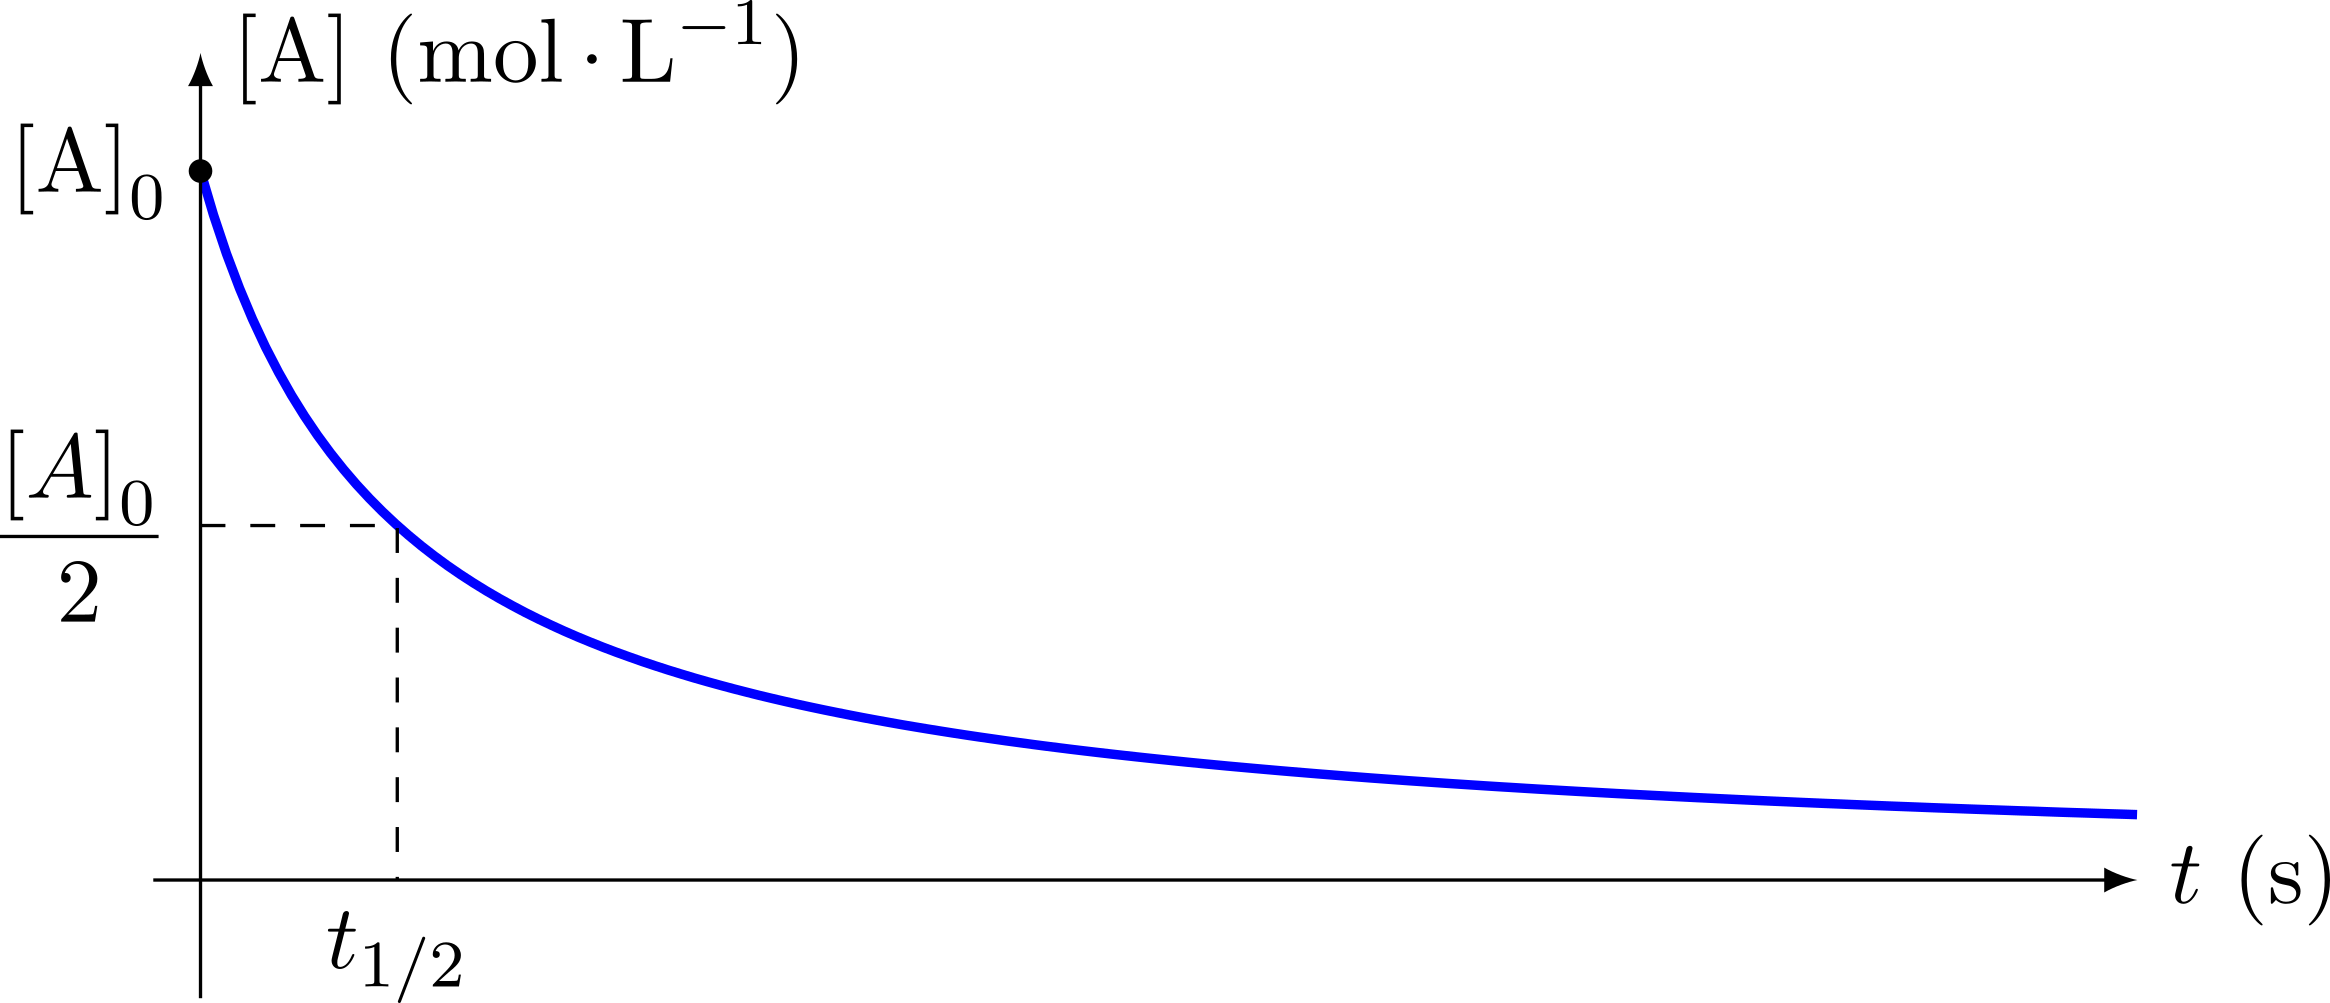
\includegraphics[width=.5\linewidth, draft=true]{ordre2}
% 	}{
% 		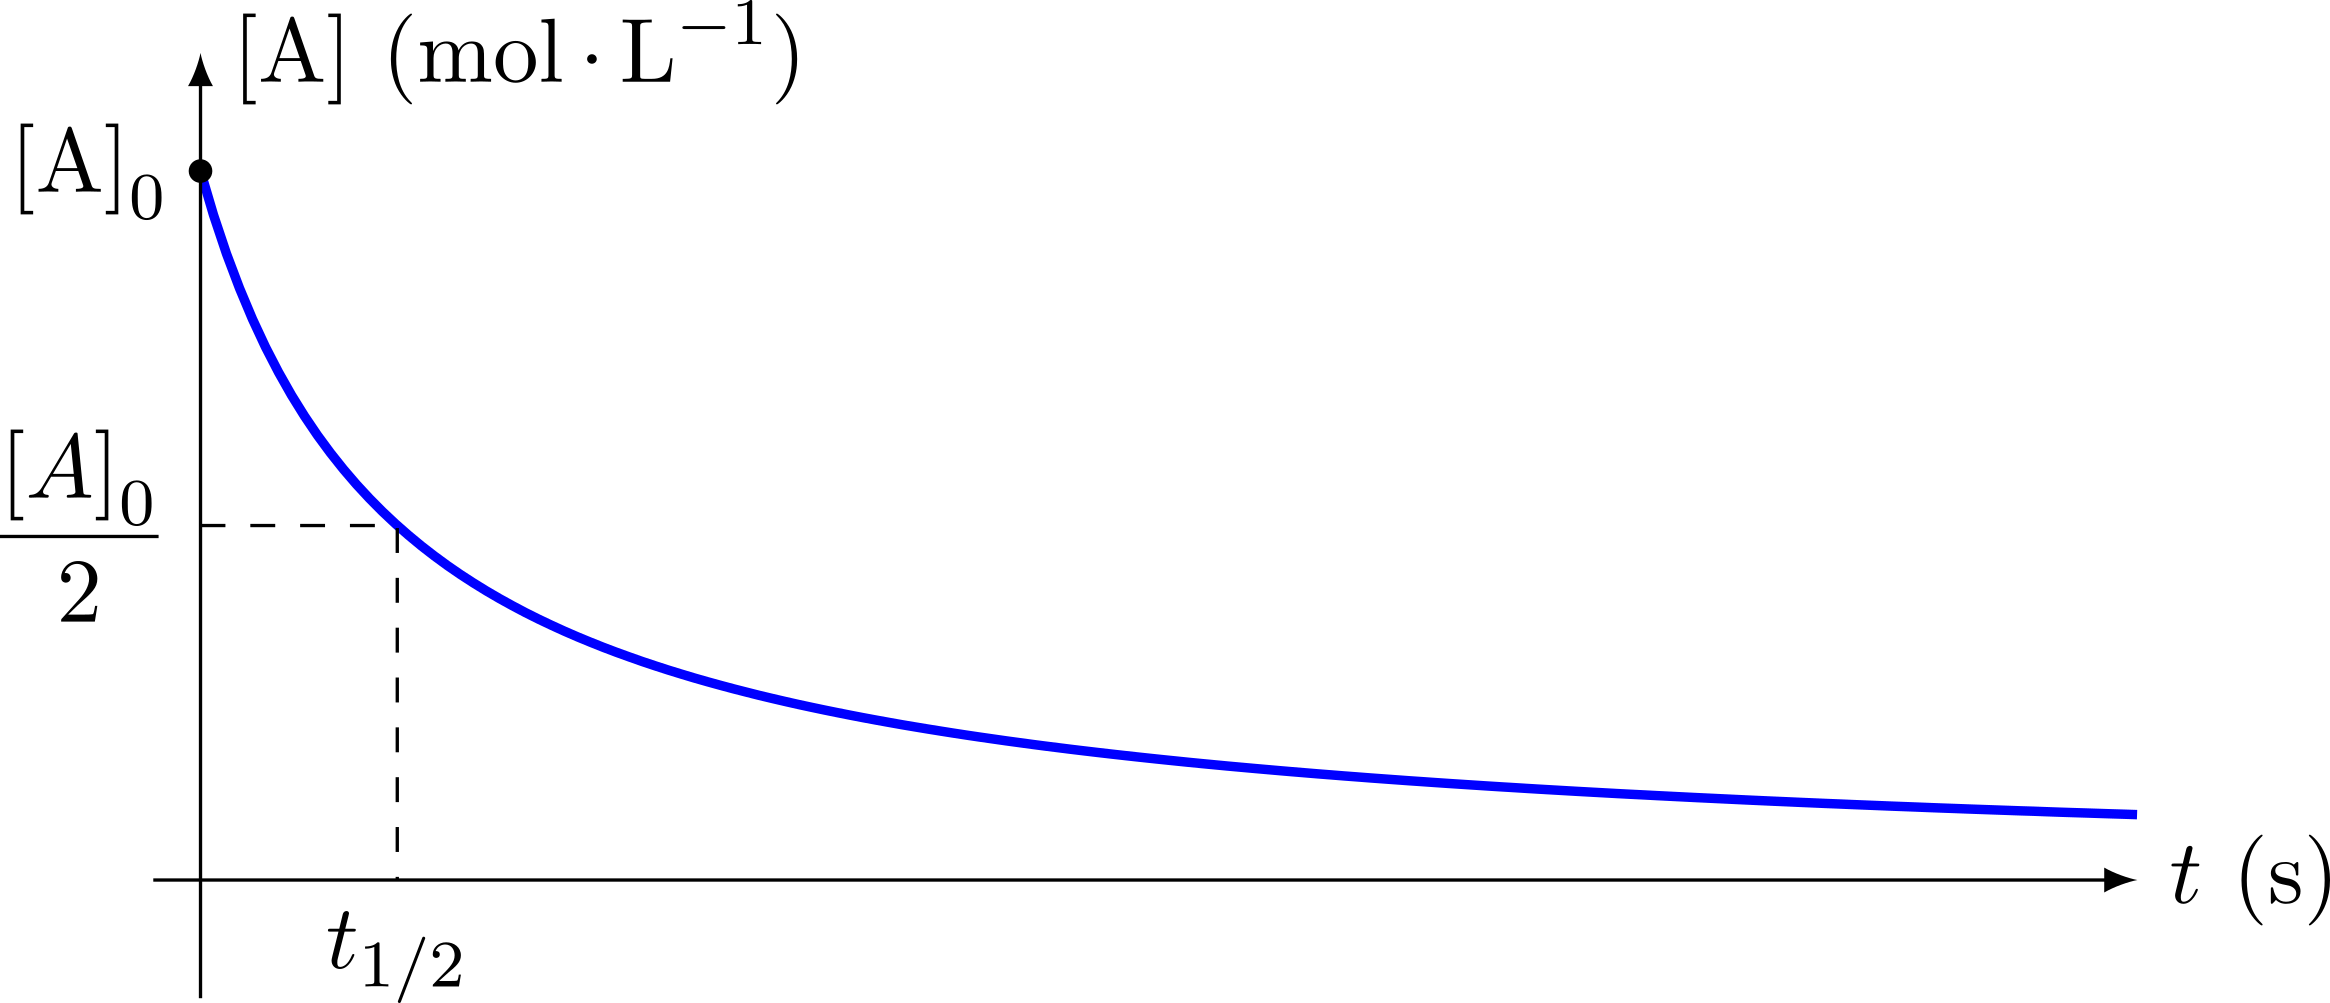
\includegraphics[width=.5\linewidth]{ordre2}
% 	}%
% 	\captionof{figure}{Ordre 2}
% \end{center}
%
% \subsubsection{Temps de demi-réaction}
% Dans le cas où A est le réactif limitant, et donc que sa concentration est nulle
% à la fin de la réaction (comme sur le graphique), on a par définition
% \psw{%
% 	\begin{gather*}
% 		[{\ce{A}}](t_{1/2}) = \frac{[{\ce{A}}]_0}{2}
% 		\Lra
% 		\frac{[{\ce{A}}]_0}{1 + kat_{1/2}[{\ce{A}}]_0} = \frac{[{\ce{A}}]_0}{2}
% 		\\\Lra
% 		1 + kat_{1/2}[{\ce{A}}]_0 = 2
% 		\Lra
% 		\boxed{t_{1/2} = \frac{1}{ka[{\ce{A}}]_0}}
% 	\end{gather*}
% }

\subsection{Expérimentalement}

\begin{tcb*}[breakable](tool){En pratique face à des données}
	\begin{itemize}
		\item[b]{Méthode différentielle}~: on travaille sur la vitesse, dérivée de
		      $x(t)$~;
		      \begin{itemize}
			      \item On a $[\ce{A}](t)$ ou $x(t)$ et $t$~;
			      \item On détermine $v = \frac{1}{\nu_{\ce{A}}}\dv{[\ce{A}]}{t}$~;
			      \item On \textbf{trace $v$ en fonction de $[\ce{A}]$}~:
			            \psw{%
				            \[
					            v = k[\ce{A}]^q
					            \quad \Ra \quad
					            \ln v = \ln k + q \ln [\ce{A}]
				            \]
			            }%
			            \vspace{-20pt}
			      \item \leftcenters{%
				            On a alors
			            }{%
				            \psw{
					            $y\tikzmark{ynd} =
						            a\tikzmark{and}x\tikzmark{xnd} + b\tikzmark{bnd}$
					            \tikz[remember picture, overlay]
					            \draw[-stealth, transform canvas={xshift=-6pt,
								            yshift=-6pt}]
					            (pic cs:ynd) --++ (-10pt,-10pt)
					            node[anchor=north east] {$\ln v$}
					            ; \tikz[remember picture, overlay]
					            \draw[-stealth, transform canvas={xshift=-5pt,
								            yshift=-6pt}]
					            (pic cs:and) --++(-5pt,-10pt)
					            node[anchor=north] {$q$}
					            ; \tikz[remember picture, overlay]
					            \draw[-stealth, transform canvas={xshift=0pt,
								            yshift=-6pt}]
					            (pic cs:xnd) --++(5pt,-10pt)
					            node[anchor=north] {$\ln [\ce{A}]$}
					            ; \tikz[remember picture, overlay]
					            \draw[-stealth, transform canvas={xshift=3pt,
								            yshift=-6pt}]
					            (pic cs:bnd) --++(10pt,-10pt)
					            node[anchor=north west] {$\ln k$}
					            ;
				            }
			            }%
			            \vspace{20pt}
			      \item On a alors \textbf{accès à $k$ et à l'ordre (partiel) sur
				            \ce{A}}.
		      \end{itemize}
		\item[b]{Méthode intégrale}~: on travaille sur la concentration, intégrée de
		      l'équation différentielle~;
		      \begin{itemize}
			      \item On a directement $t$ et $[A](t)$, et \textbf{on suppose
				            l'ordre de
				            \ce{A}}~;
			      \item On réalise la \textbf{régression associée à chaque ordre}~;
			      \item On prend la meilleure régression en ne se fiant pas qu'au
			            $r^2$~;
			      \item On a alors accès à $k$ et à l'ordre.
		      \end{itemize}
		\item[b]{Méthode de demi-réaction}~: on travaille sur le temps de
		      demi-réaction~;
		      \begin{itemize}
			      \item On a réalisé des expériences en faisant \textbf{varier
				            $[\ce{A}]_0$}~;
			      \item On possède à chaque fois le temps de demi-réaction~;
			      \item On étudie la dépendance de $t_{1/2}$ à $[\ce{A}]_0$~:
			            \begin{itemize}
				            \item \psw{%
					                  si $t_{1/2}$ est proportionnel à $[\ce{A}]_0$, alors
					                  la cinétique est d'ordre 0.
				                  }%
				            \item \psw{%
					                  si $t_{1/2}$ est indépendant de $[\ce{A}]_0$, alors
					                  la cinétique est d'ordre 1.
				                  }%
				            \item \psw{%
					                  si $t_{1/2}$ est inversement proportionnel à
					                  $[\ce{A}]_0$, alors la cinétique est d'ordre 2.
				                  }%
			            \end{itemize}
		      \end{itemize}
	\end{itemize}
\end{tcb*}

\subsection{Résumé}

\begin{tcb}[label=ror:resumeordre, tabularx={l|Y|Y|Y}](ror)
	{Ordres sur un unique réactif}
	&
	\vspace{8pt}
	\textbf{Ordre 0 en A} &
	\vspace{8pt}
	\textbf{Ordre 1 en A} &
	\vspace{8pt}
	\textbf{Ordre 2 en A}
	\\\hline
	\rotatebox[origin=c]{90}{$v$, $[k]$} &
	\psw{%
		\begin{center}
			$v = k$\\
			$k$ en $\si{mol.L^{-1}.s^{-1}}$
		\end{center}
	}%
	&
	\psw{%
		\begin{center}
			$v = k[{\ce{A}}]$\\
			$k$ en $\si{s^{-1}}$
		\end{center}
	}%
	&
	\psw{%
		\begin{center}
			$v = k[{\ce{A}}]^2$\\
			$k$ en $\si{mol^{-1}.L.s^{-1}}$
		\end{center}
	}%
	\\\hline
	\rotatebox[origin=c]{90}{ED} &
	\psw{\[\dv{[{\ce{A}}]}{t} + \abs{\nu_{\ce{A}}}k = 0\]}
	&
	\psw{\[\dv{[{\ce{A}}]}{t} + \abs{\nu_{\ce{A}}}k [{\ce{A}}] = 0\]}
	&
	\psw{\[\dv{[{\ce{A}}]}{t} + \abs{\nu_{\ce{A}}}k [{\ce{A}}]^2 = 0\]}
	\\\hline
	\rotatebox[origin=c]{90}{Solution} &
	\psw{\[\boxed{[{\ce{A}}](t) = [{\ce{A}}]_0 - \abs{\nu_{\ce{A}}}kt}\]}
	&
	\psw{\[\boxed{[{\ce{A}}](t) = [{\ce{A}}]_0\exp(-\abs{\nu_{\ce{A}}}kt)}\]}
	&
	\psw{\[\boxed{[{\ce{A}}](t) = \frac{[{\ce{A}}]_0}{1 + \abs{\nu_{\ce{A}}}kt[{\ce{A}}]_0}}\]}
	\\\hline
	\rotatebox[origin=c]{90}{$t_{1/2}$} &
	\psw{\[t_{1/2} = \frac{[{\ce{A}}]_0}{2\abs{\nu_{\ce{A}}}k}\]}
	&
	\psw{\[t_{1/2} = \frac{\ln 2}{\abs{\nu_{\ce{A}}}k}\]}
	&
	\psw{\[t_{1/2} = \frac{1}{\abs{\nu_{\ce{A}}}k[{\ce{A}}]_0}\]}
	\\\hline
	\rotatebox[origin=c]{90}{Graphiques} &
	\begin{center}
		\sswitch{
			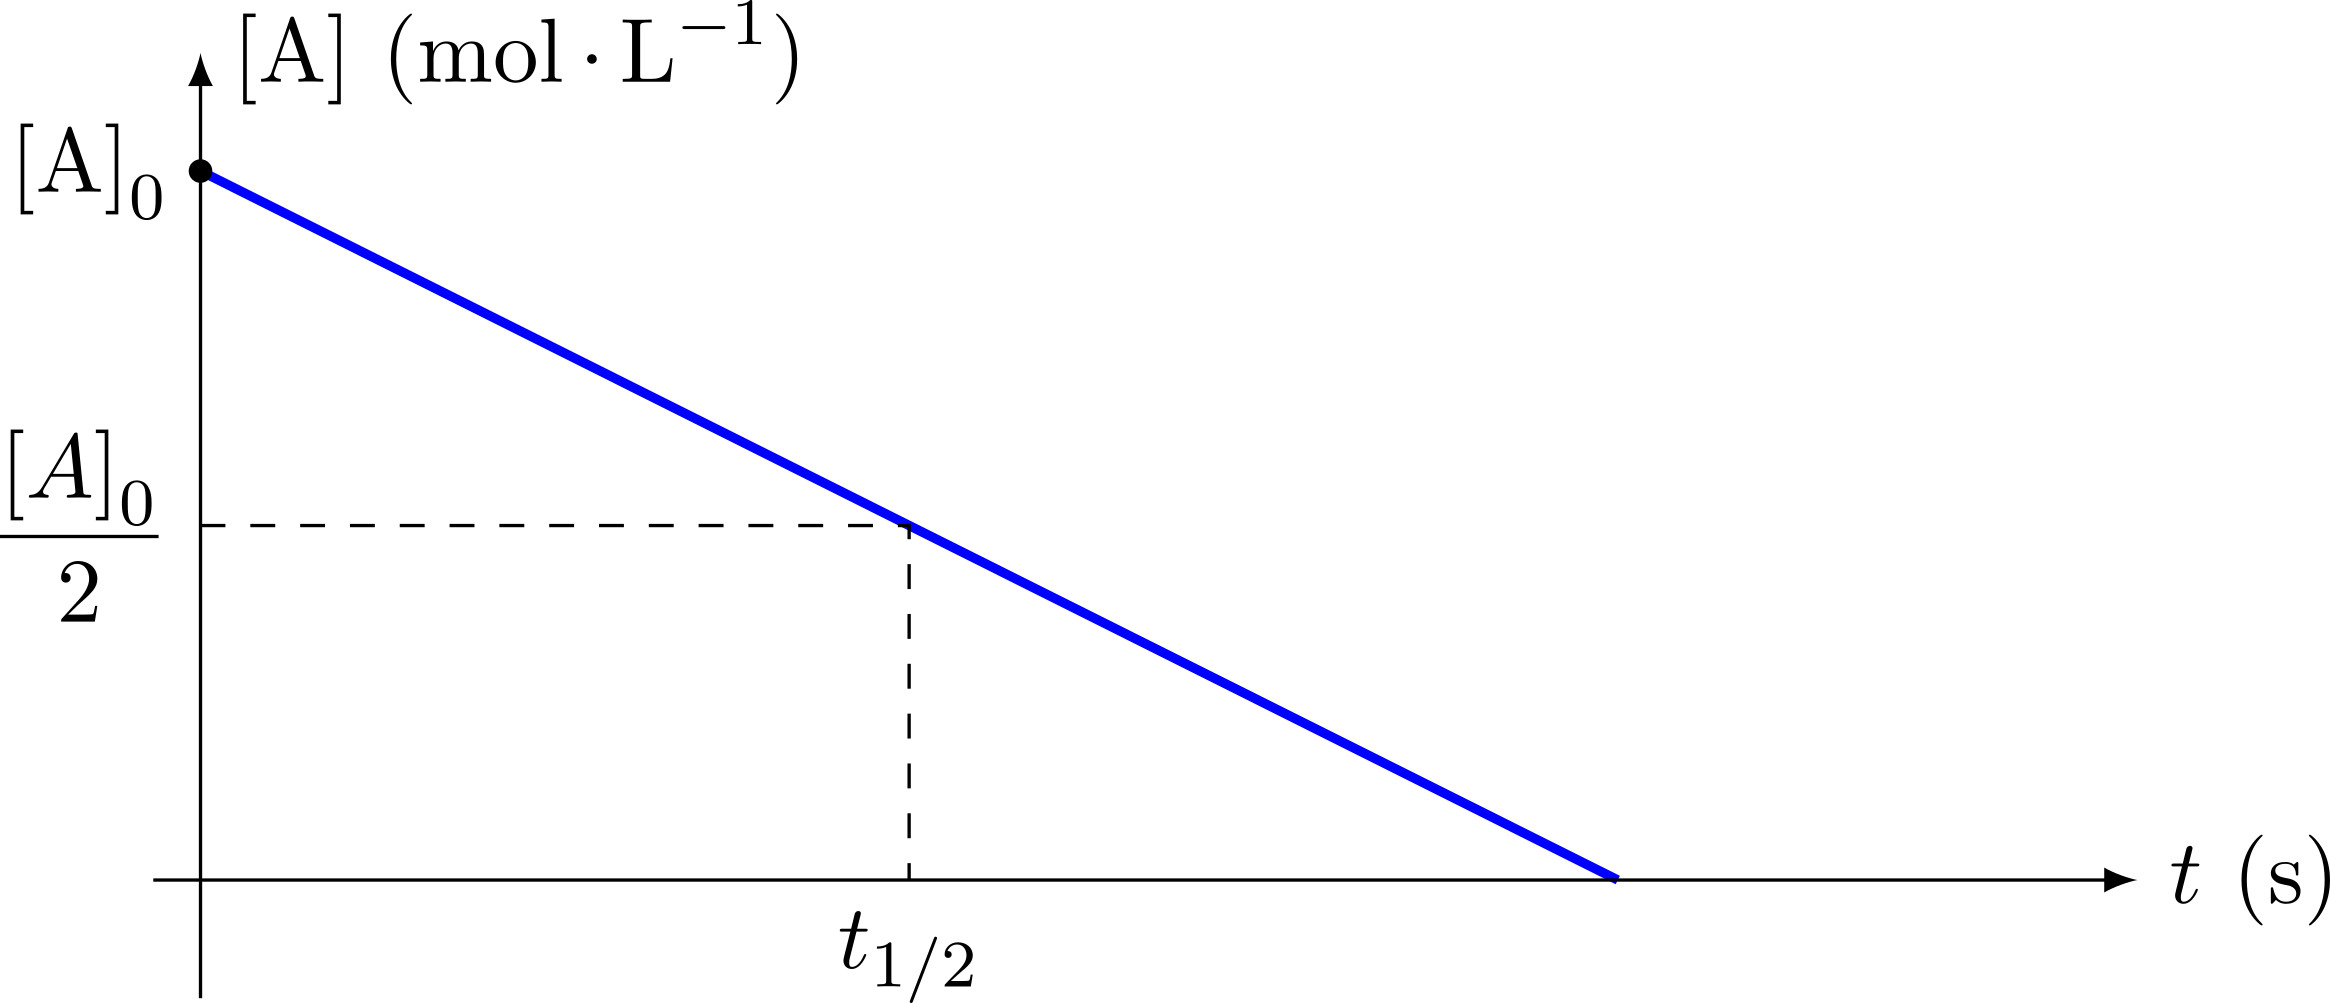
\includegraphics[width=\linewidth, draft=true]{ordre0}
		}{
			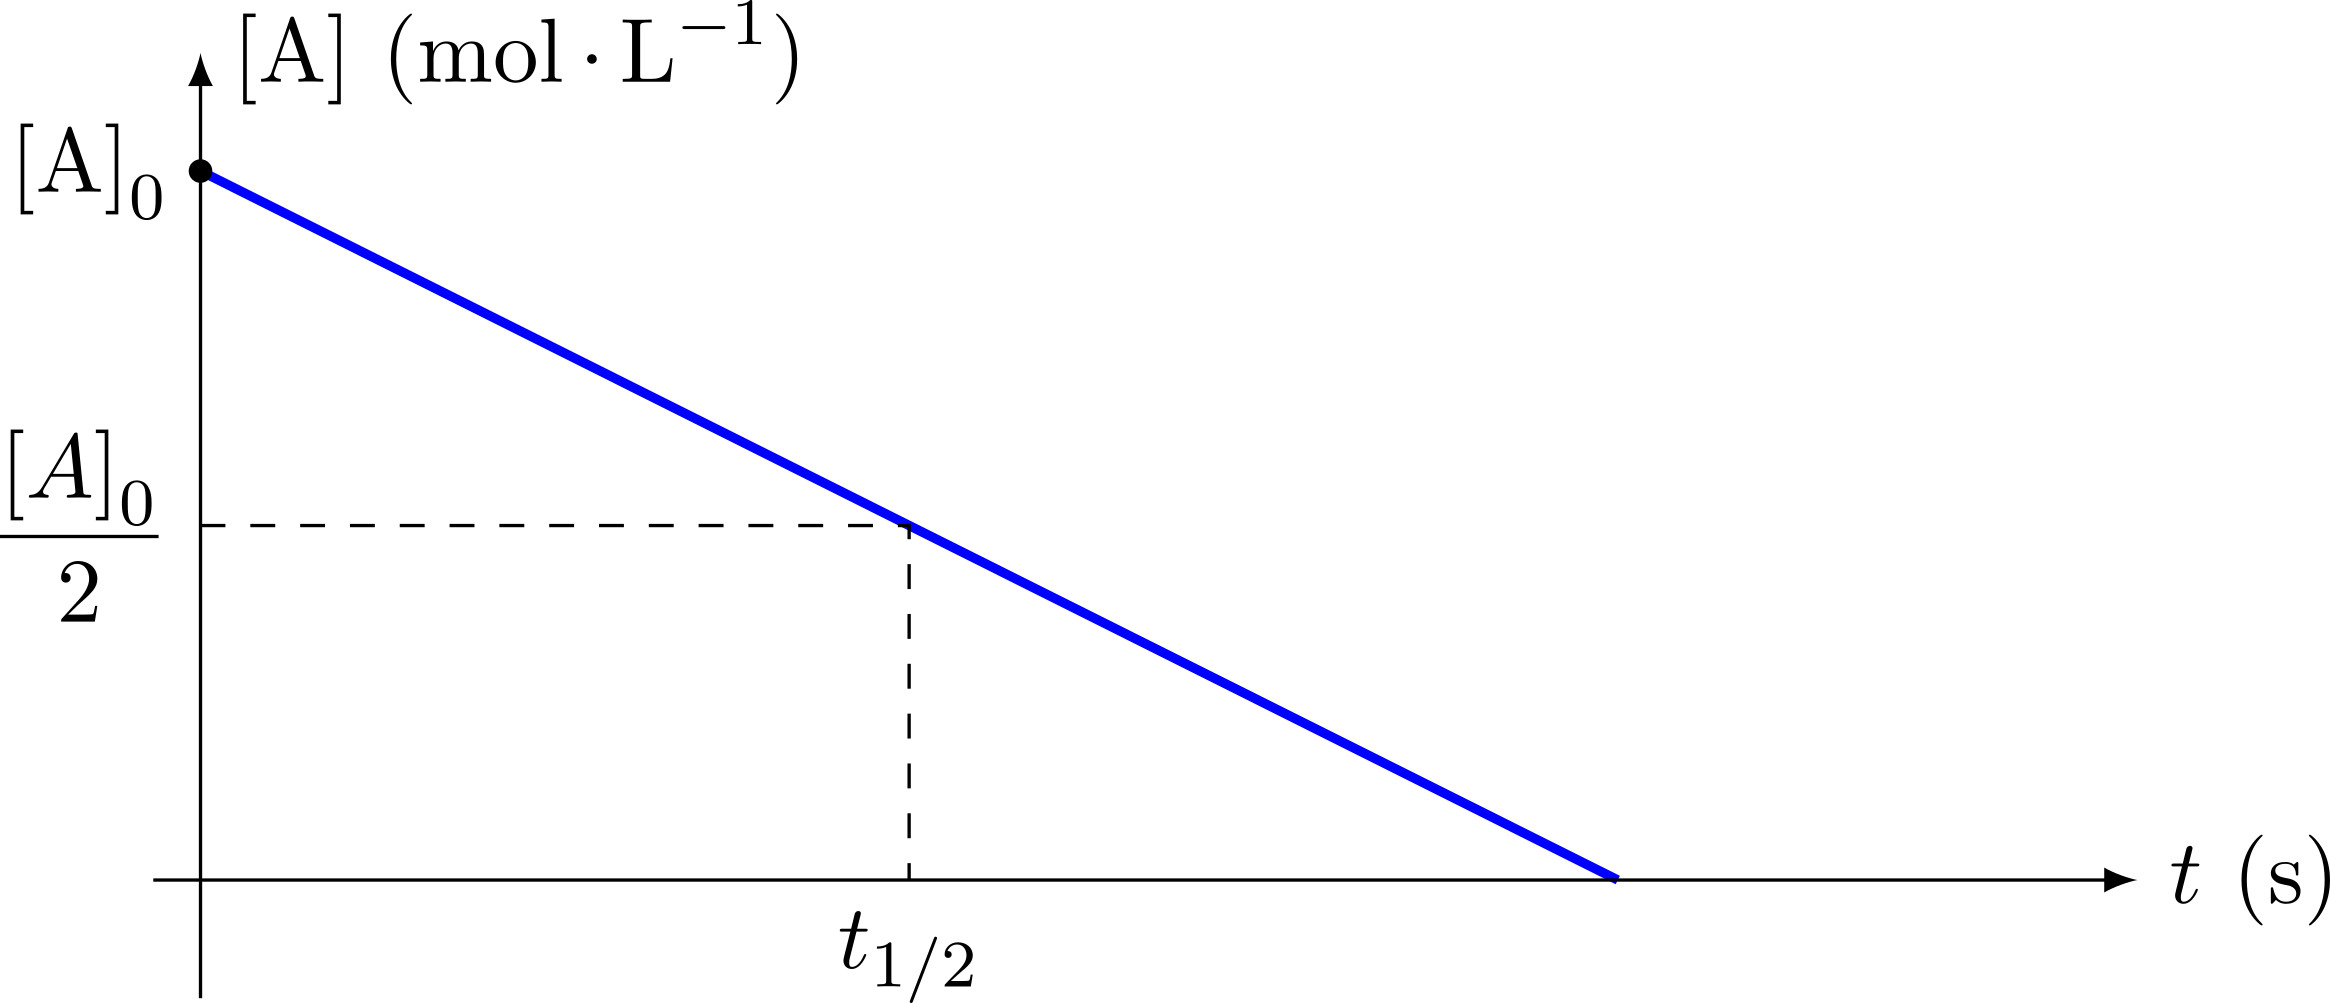
\includegraphics[width=\linewidth]{ordre0}
		}%
		\captionof{figure}{Ordre 0}
	\end{center}
	&
	\begin{center}
		\sswitch{
			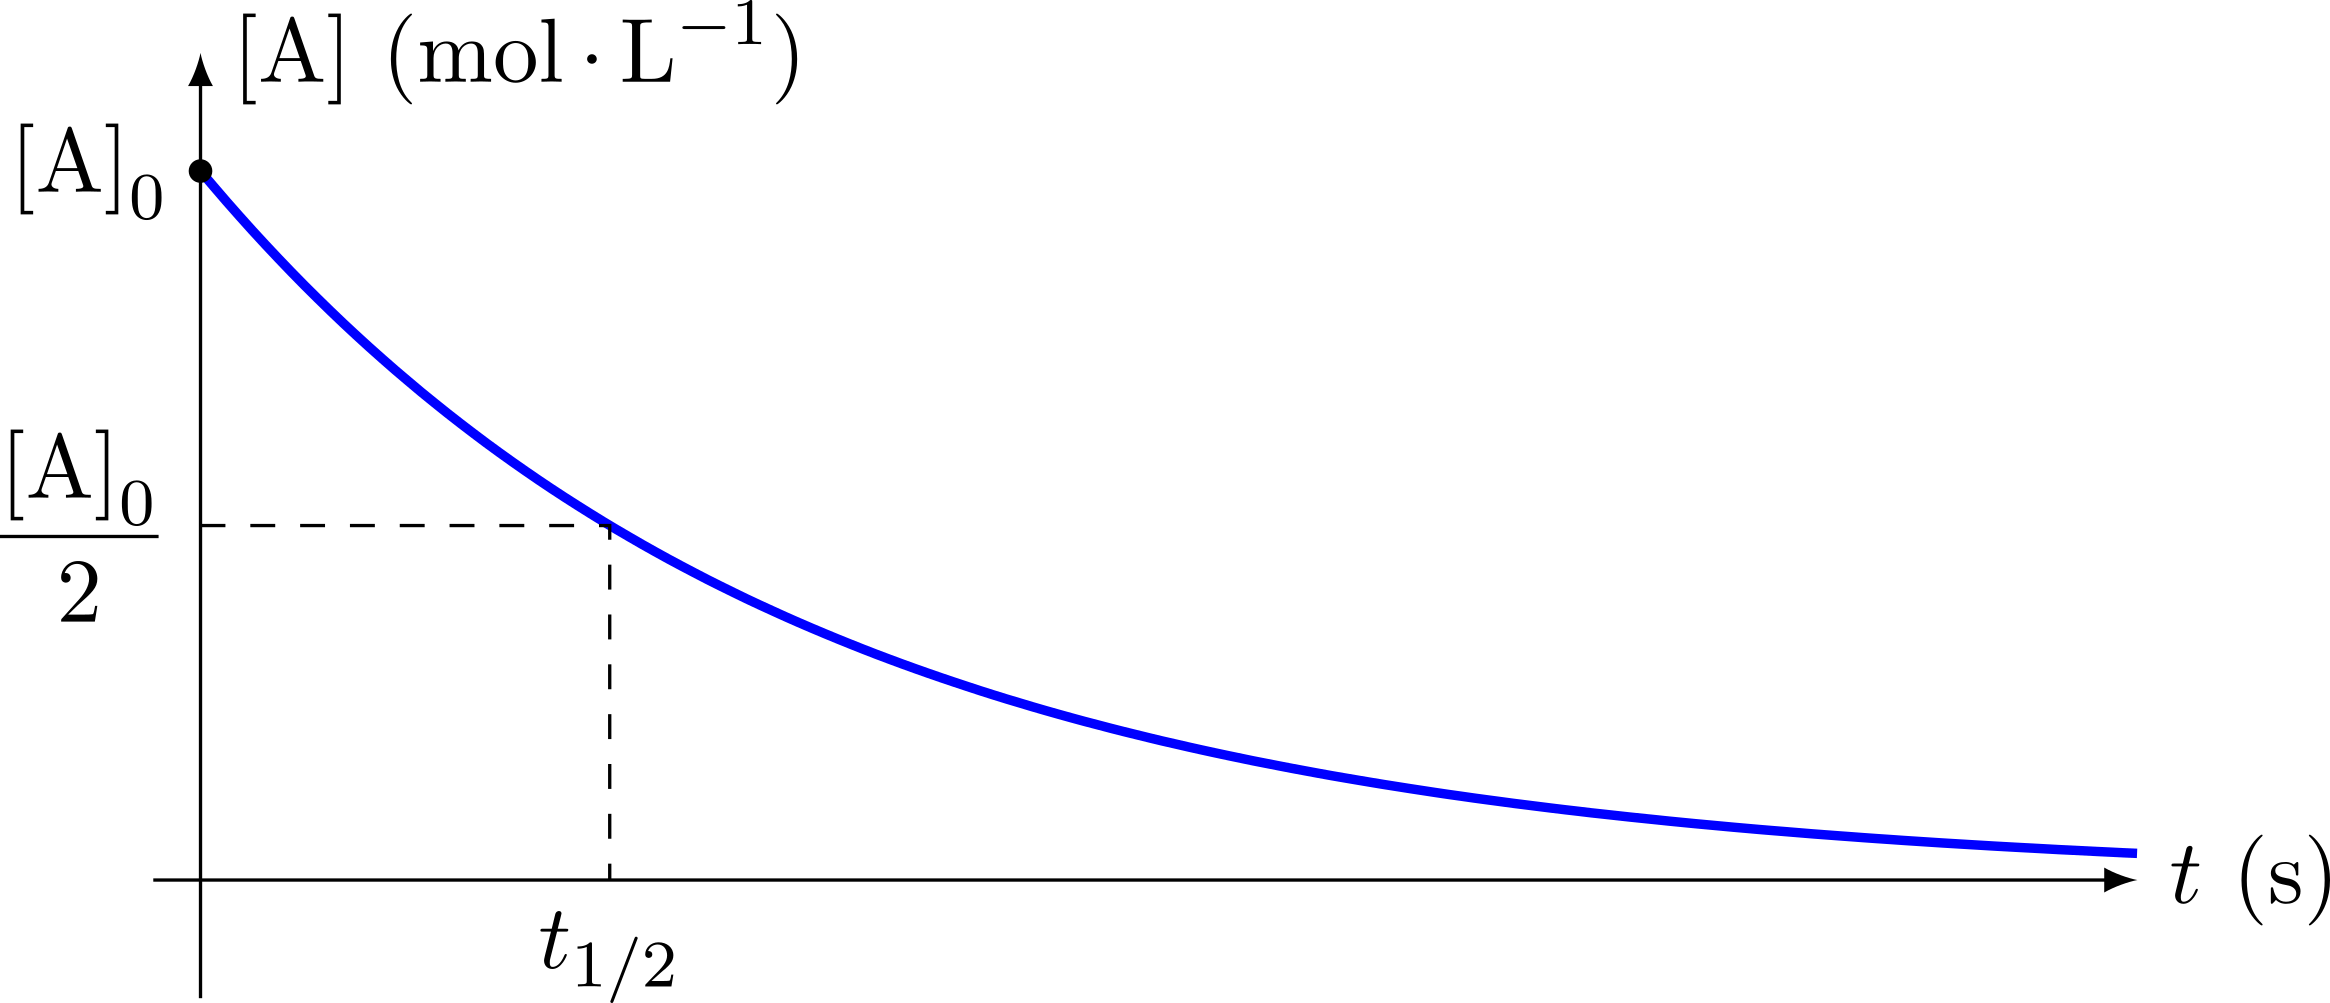
\includegraphics[width=\linewidth, draft=true]{ordre1}
		}{
			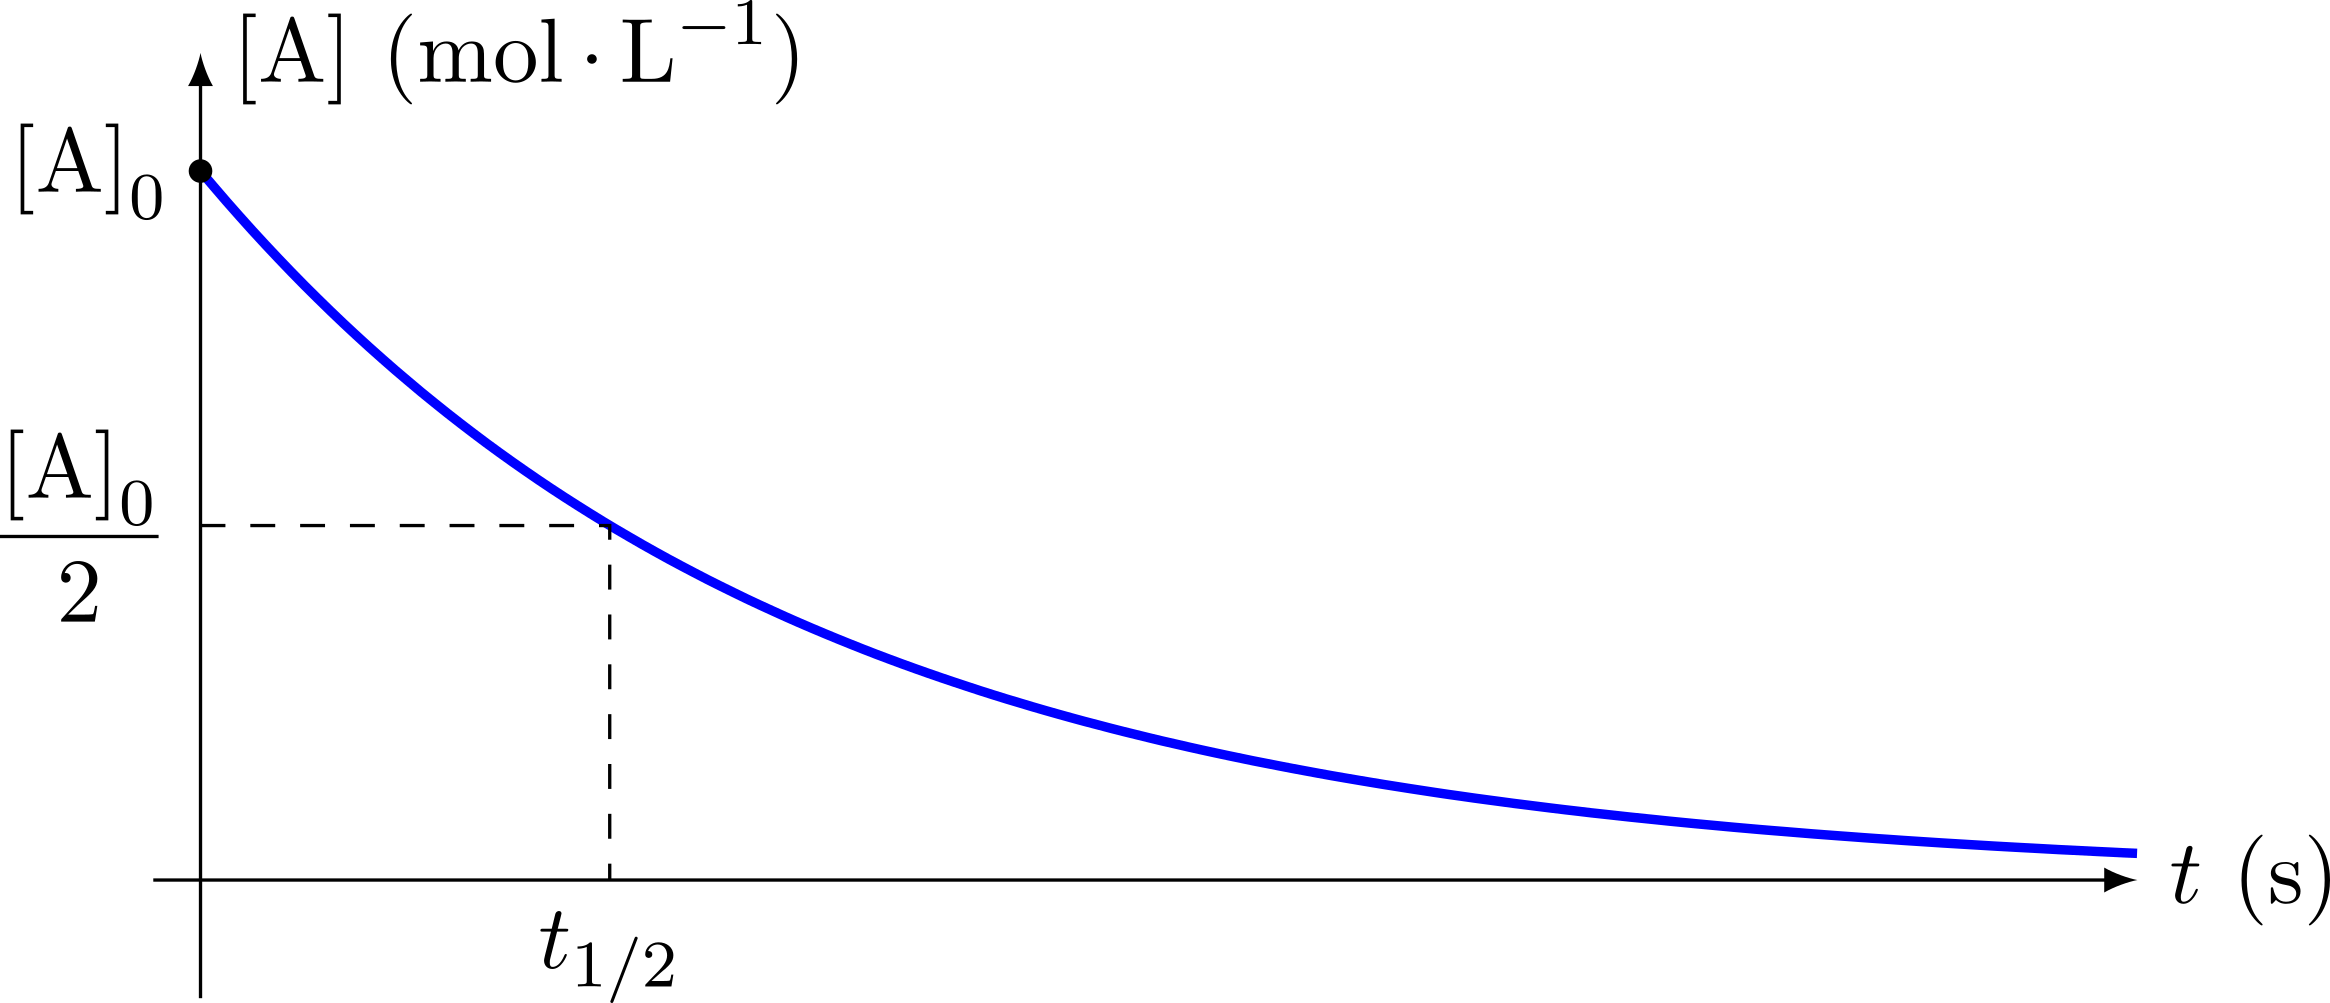
\includegraphics[width=\linewidth]{ordre1}
		}%
		\captionof{figure}{Ordre 1}
	\end{center}
	&
	\begin{center}
		\sswitch{
			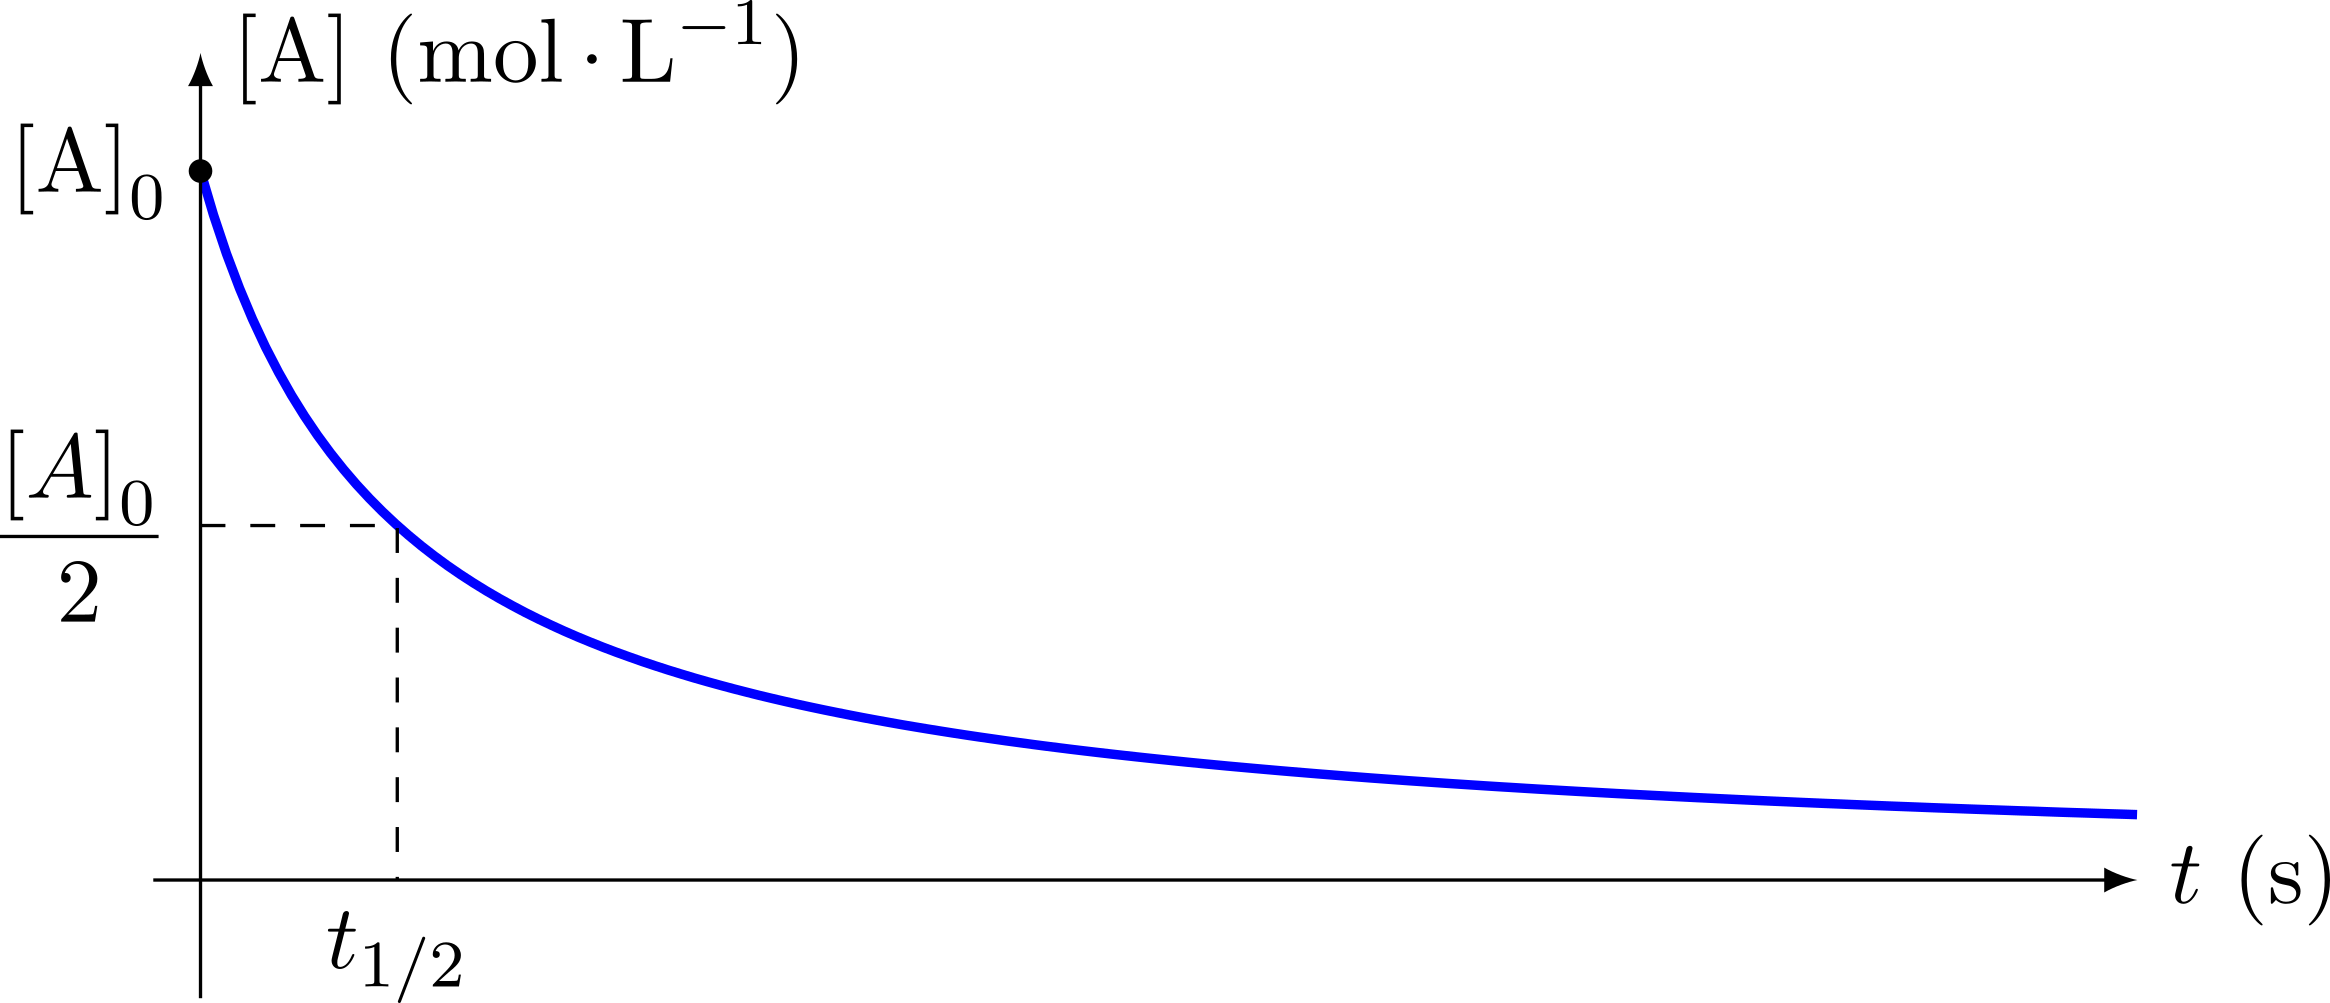
\includegraphics[width=\linewidth, draft=true]{ordre2}
		}{
			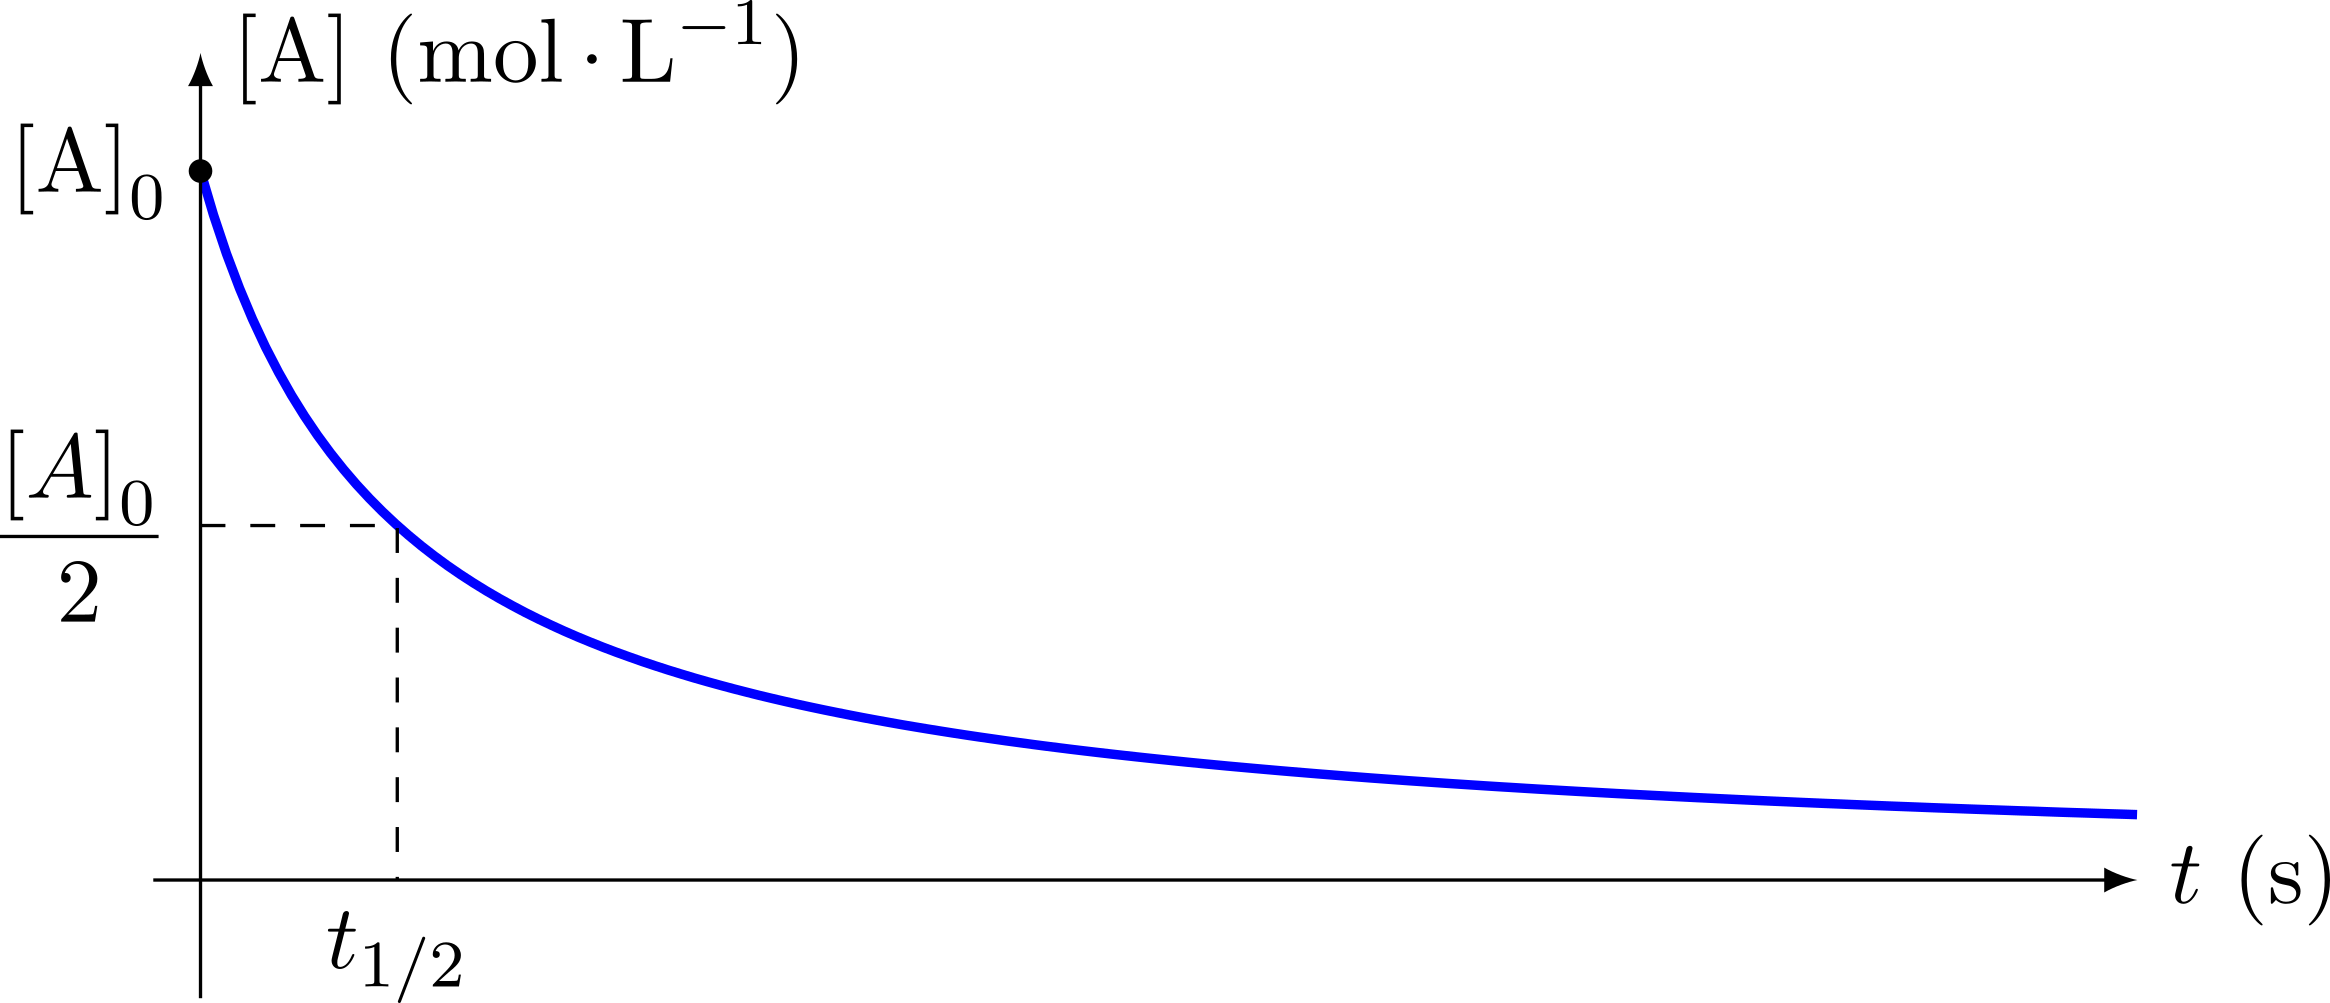
\includegraphics[width=\linewidth]{ordre2}
		}%
		\captionof{figure}{Ordre 2}
	\end{center}
\end{tcb}

\begin{tcb*}[breakable](impo)"bomb"{$k$ ou $k\ind{app}$}
	Les exemples précédents sont donnés pour une réaction dont la loi de vitesse
	\textbf{ne dépend que d'un réactif}. Dans la pratique, une loi de vitesse va
	le plus souvent dépendre de \textbf{deux réactifs}, mais on aura réalisé une
	\textbf{dégénérescence d'ordre} ou réalisé une expérience en
	\textbf{proportions stœchiométriques}.
	\smallbreak
	Il faudra alors être particulièrement vigilant-e sur la \textbf{constante et
		l'ordre obtenus}~: est-ce bien $k$ de la loi de vitesse générale, ou un
	$k\ind{app}$ d'une situation spécifique~? $q$ l'ordre global en \ce{A}, ou
	l'ordre global $m = p+q$…~?
\end{tcb*}

% \begin{tcn}(coro)<ctb>"trans"{Transition}
% 	Comment faisons nous en pratique un suivi expérimental, et notamment quelles
% 	sont les lois mathématiques derrière les suivis par grandeurs physiques~?
% \end{tcn}

\section{Méthodes de suivi cinétique expérimental}
\subsection{Dosage par titrage}
\subsubsection{Définition}
\begin{tcb}[label=def:titrage](defi){Suivi cinétique par titrage}
	La méthode chimique consiste à prélever un faible volume d'essai du système
	étudié à intervalles de temps régulier~; la concentration des espèces
	chimiques d'intérêt est alors \textbf{titrée} sur ce volume d'essai.
\end{tcb}
Les méthodes de titrage seront détailles avec plus de précision plus tard dans
l'année, à la fois en cours et en TP. Ce qu'il faut en retenir pour le moment,
c'est qu'elle permet une détermination \textbf{absolue} de la concentration,
mais qu'elle présente certains forts désavantages~: c'est une méthode
\begin{itemize}
	\item[b]{destructive}~: chaque prélèvement diminue le volume du système
	      initial et la quantité de matière de produit ou réactif selon la
	      méthode~;
	\item[b]{laborieuse}~: il faut faire autant de dosages que de points de
	      mesures~;
	\item[b]{non continue}~: on n'a accès qu'à un nombre limité de points de
	      mesure~;
	\item[b]{lente}~: un dosage prend, au mieux et environ \SI{5}{min}.
\end{itemize}
Il faut donc notamment \textbf{arrêter la réaction} dans le volume d'essai, pour
que le prélèvement à un instant $t$ dosé environ \SI{5}{min} plus tard
corresponde quand même à un point de mesure à l'instant $t$. Pour ce faire, il
faut avoir recours à une \textbf{trempe chimique}.

\subsubsection{La trempe chimique}
La trempe chimique est le nom d'un processus destiné à figer l'état d'un
systèmes physico-chimiques. On recense trois méthodes de trempe~:
\begin{enumerate}
	\item \textbf{La dilution}~: la vitesse de réaction étant une fonction
	      croissante de la concentration en réactif, \textbf{diluer le volume
		      d'essai} d'un facteur 10 à 100 permet de ralentir fortement la cinétique
	      de la réaction.
	\item \textbf{Le refroidissement}~: la constante de vitesse croît avec la
	      température, et par conséquent abaisser la température du volume d'essai
	      permet de ralentir la cinétique de la réaction qui s'y passe. C'est une
	      méthode particulièrement intéressante quand on part de réactions
	      initialement hautes en températures, pour abaisser par exemple de
	      \SI{100}{\degreeCelsius} à \SI{0}{\degreeCelsius} la solution.
	\item \textbf{La disparition d'un réactif}~: il est également possible de
	      faire disparaître l'un des réactifs (celui qui ne sera pas dosé) en
	      réalisant une réaction rapide et totale avant d'effectuer le dosage. Par
	      exemple, une réaction ayant pour réactif un acide peut être interrompue
	      en modifiant le pH du volume par ajout d'une base forte, comme
	      $\ce{HO-}$.
\end{enumerate}

\subsection{Dosage par étalonnage}
Comme introduit dans la première section, il est possible de sonder
indirectement la concentration en une espèce \textit{via} l'évolution d'une
grandeur physique. Pour que le suivi soit quantitatif, il faut que la valeur de
la grandeur mesurée soit comparée à une valeur de référence, un étalon. Pour
qu'un dosage par étalonnage soit efficace, il faut~:
\begin{itemize}
	\item que la grandeur évolue de manière sensible lorsque l'on passe du
	      réactif au produit. Si le réactif a la même conductivité que le produit
	      formé, on comprend aisément qu'un suivi conductimétrique ne nous sera
	      d'aucune aide…
	\item que la grandeur varie de manière simple et prédictible avec la
	      concentration (si possible de manière linéaire).
\end{itemize}

\subsubsection{Spectrophotométrie}
\begin{tcb}[label=loi:berrlambert](loi){Loi de \textsc{Beer-Lambert}}
	On relie l'intensité lumineuse transmise par une espèce à une longueur
	d'onde donnée avec la concentration de l'espèce colorée en solution grâce à
	la loi de \textbf{Beer-Lambert}~:
	\[
		\boxed{
			A = \log \left( \frac{I_0}{I} \right) = \sum_{i=1}^{N}\epsilon_i
			\ell c_i
		}%
	\]
	\begin{itemize}
		\item $A$ est l'\textbf{absorbance}, sans dimension~;
		\item $I_0$ l'intensité lumineuse \textbf{incidente}, en $\si{W.m^{-2}}$~;
		\item $I$ l'intensité lumineuse \textbf{en sortie}, aussi en
		      $\si{W.m^{-2}}$~;
		\item $\epsilon_i$ le coefficient d'extinction molaire de l'espèce X$_i$
		      à la longueur d'onde $\lambda$ (dépend de l'espèce et un peu du
		      solvant et de $T$)~;
		\item $\ell$ la distance traversée par le faisceau, en \si{m} (souvent
		      \si{cm})~;
		\item $c$ la concentration de l'espèce absorbante X$_i$, en
		      $\si{mol.L^{-1}}$.
	\end{itemize}
	\begin{center}
		C'est une loi \textbf{additive} et \textbf{linéaire}.
	\end{center}
\end{tcb}

\subsubsection{Conductimétrie}
\begin{tcb}[label=loi:kohlrausch](loi){Loi de \textsc{Kohlrausch}}
	Les ions conduisant le courant, il est possible dans certains cas de suivre
	l'avancement de la réaction en mesurant l'évolution de la conductivité de la
	solution associée à la concentration des ions grâce à la \textbf{loi de
		Kohlrausch}~:
	\[\boxed{\sigma = \sum_{i=1}^{N}\lambda_ic_i}\]
	\begin{itemize}
		\item $\sigma$ est la conductivité de la solution, en
		      $\si{\Omega^{-1}.m^{-1}}$~;
		\item $\lambda_i$ est la conductivité molaire ionique de l'espèce X$_i$,
		      dépendante de l'espèce et de la température, en
		      $\si{\Omega^{-1}.m^{-1}.mol^{-1}.L}$~;
		\item $c_i$ est la concentration molaire en l'espèce X$_i$, en
		      $\si{mol.L^{-1}}$.
	\end{itemize}
	\begin{center}
		C'est une loi \textbf{additive} et \textbf{linéaire}.
	\end{center}
\end{tcb}

\end{document}
